\documentclass[double,12pt]{psutex}

\usepackage[hyphens]{url}
\usepackage{geometry}
\usepackage{verbatim}
\usepackage[table]{xcolor}
\usepackage{subcaption}
\usepackage{graphicx}
\usepackage{amsmath,amsthm,amssymb}
\usepackage{stmaryrd}
\usepackage{tikz}
\usepackage{array,multirow}
\usepackage{hyperref}
\usepackage[capitalize]{cleveref}
\usepackage{booktabs}
\usepackage{threeparttable}
\usepackage{wasysym}
\usepackage{listings}
\usepackage[noadjust]{cite}
\usepackage[multiple]{footmisc}
\usepackage{algorithmic}
\usepackage{textcomp}
\usepackage[inline]{enumitem}
\usepackage[normalem]{ulem}
\usepackage{listing}
\usepackage{xspace}
\usepackage[most]{tcolorbox}

\theoremstyle{definition}
\newtheorem{definition}{Definition}

\newcommand{\paragraphx}[1]{\emph{#1.}}

\newcommand{\tagcolor}{C}

\newcommand{\vt}{\mathit{vt}}
\newcommand{\pt}{\mathit{pt}}
\newcommand{\lt}{\mathit{lt}}
\newcommand{\lts}{\overline{\lt}}
\newcommand{\nt}{\mathit{nt}}
\newcommand{\PCT}{\mathcal{P}}

\newcommand{\trule}[2]{#1 \leftarrow #2}

\newcommand{\truledef}[1]{
  & \multispan{3} \(#1\) \\}

\newcommand{\assert}[1]{& & & \multispan{2} \(\mathbf{assert} ~ #1\) \hfill \\}
\newcommand{\letin}[1]{& & & \multispan{2} \(\mathit{let} ~ #1 ~ \mathit{in}\) \\}

\newcommand{\caseof}[1]{\textnormal{case } #1 \textnormal{ of}}
\newcommand{\caseentry}[2]{& & & #1 \Rightarrow #2}

\newcommand{\optional}[1]{\fcolorbox{black}{gray!20}{#1}}
\newcommand{\settag}[2]{\boldsymbol{#1} & \longleftarrow & & \mathit{#2}\\}
\newcommand{\settagopt}[2]{\optional{\(\boldsymbol{#1}\)} & \longleftarrow & & \mathit{#2}\\}

%%% Tag Rules %%%
\newcommand{\loadtname}{\mathbf{LoadT}}
\newcommand{\loadtargs}{\PCT, \pt, \vt, \overline{\lt}}
\newcommand{\loadtres}{\vt'}
\newcommand{\loadt}{\loadtname(\loadtargs)}

\newcommand{\storetname}{\mathbf{StoreT}}
\newcommand{\storetargs}{\PCT, \pt, \vt_1, \vt_2, \overline{\lt}}
\newcommand{\storetres}{\PCT',\vt',\overline{\lt}'}
\newcommand{\storet}{\storetname(\storetargs)}

\newcommand{\consttname}{\mathbf{ConstT}}
\newcommand{\consttres}{\vt}
\newcommand{\constt}{\consttname}

\newcommand{\unoptname}{\mathbf{UnopT}}
\newcommand{\unoptargs}{\PCT, \vt}
\newcommand{\unoptres}{\vt}
\newcommand{\unopt}{\unoptname(\unoptargs)}

\newcommand{\binoptname}{\mathbf{BinopT}}
\newcommand{\binoptargs}{\PCT, \vt_1, \vt_2}
\newcommand{\binoptres}{\vt'}
\newcommand{\binopt}{\binoptname(\binoptargs)}

\newcommand{\globaltname}{\mathbf{GlobalT}}
\newcommand{\globaltargs}{id, s}
\newcommand{\globaltargstyped}{id \in ident, s \in \mathbb{N}}
\newcommand{\globaltres}{\pt,\vt,\overline{\lt}}
\newcommand{\globalt}{\globaltname(\globaltargs)}

\newcommand{\localtname}{\mathbf{LocalT}}
\newcommand{\localtargs}{\PCT, id, s}
\newcommand{\localtargstyped}{\PCT, id \in ident, s \in \mathbb{N}}
\newcommand{\localtres}{\pt,\vt,\overline{\lt}}
\newcommand{\localt}{\localtname(\localtargs)}

\newcommand{\vartname}{\mathbf{VarT}}
\newcommand{\vartargs}{\PCT, \vt}
\newcommand{\vartres}{\pt}
\newcommand{\vart}{\vartname(\vartargs)}

\newcommand{\malloctname}{\mathbf{MallocT}}
\newcommand{\malloctargs}{\PCT, \vt}
\newcommand{\malloctres}{\PCT',\pt,\optional{\(\vt,\overline{\lt}\)}}
\newcommand{\malloct}{\malloctname(\malloctargs)}

\newcommand{\freetname}{\mathbf{FreeT}}
\newcommand{\freetargs}{\PCT, \vt}
\newcommand{\freetres}{\PCT',\pt,\optional{\(\vt,\overline{\lt}\)}}
\newcommand{\freet}{\freetname(\freetargs)}

\newcommand{\picasttname}{\mathbf{PICastT}}
\newcommand{\picasttargs}{\PCT, \pt, \optional{\(\vt, \overline{\lt}\)}}
\newcommand{\picasttres}{\PCT',\vt}
\newcommand{\picastt}{\picasttname(\picasttargs)}

\newcommand{\ipcasttname}{\mathbf{IPCastT}}
\newcommand{\ipcasttargs}{\PCT, \vt_1, \optional{\(\vt_2, \overline{\lt}\)}}
\newcommand{\ipcasttres}{\PCT',\pt}
\newcommand{\ipcastt}{\ipcasttname(\ipcasttargs)}

\newcommand{\ppcasttname}{\mathbf{PPCastT}}
\newcommand{\ppcasttargs}{\PCT, \pt, \optional{\(\vt, \overline{\lt}\)}}
\newcommand{\ppcasttres}{\PCT',\pt'}
\newcommand{\ppcastt}{\picasttname(\picasttargs)}

\newcommand{\iicasttname}{\mathbf{IICastT}}
\newcommand{\iicasttargs}{\PCT, \vt_1}
\newcommand{\iicasttres}{\PCT',\pt}
\newcommand{\iicastt}{\ipcasttname(\ipcasttargs)}

\newcommand{\splittname}{\mathbf{SplitT}}
\newcommand{\splittargs}{\PCT, \vt, \optional{\(L\)}}
\newcommand{\splittres}{\PCT'}
\newcommand{\splitt}{\splittname(\splittargs)}
           
\newcommand{\jointname}{\mathbf{JointT}}
\newcommand{\jointargs}{\PCT, \optional{\(L\)}}
\newcommand{\jointres}{\PCT'}
\newcommand{\joint}{\jointname(\jointargs)}

\newcommand{\argtname}{\mathbf{ArgT}}
\newcommand{\argtargs}{\PCT, \vt, f, x}
\newcommand{\argtargstyped}{\PCT, \vt, f, x \in ident}
\newcommand{\argtres}{\vt'}
\newcommand{\argt}{\argtname(\argtargs)}

\newcommand{\callerrettname}{\mathbf{CallerRetT}}
\newcommand{\callerrettargs}{\PCT, \PCT', \vt}
\newcommand{\callerrettres}{\vt'}
\newcommand{\callerrett}{\callerrettname(\callerrettargs)}

\newcommand{\calleerettname}{\mathbf{CalleeRetT}}
\newcommand{\calleerettargs}{\PCT, \PCT', \vt}
\newcommand{\calleerettres}{\vt'}
\newcommand{\calleerett}{\calleerettname(\calleerettargs)}

%%%%%%%%%%%%%%%%%

%%% Continuations, States, Values %%%

\newcommand{\kemp}{\mathit{Kemp}}
\newcommand{\kdo}[1]{\mathit{Kdo};~ #1}
\newcommand{\kseq}[2]{\mathit{Kseq} ~ #1; ~ #2}
\newcommand{\kif}[4]{\mathit{Kif}[#1 \mid #2] ~ \mathit{join} ~ #3; ~ #4}
\newcommand{\kwhiletest}[4]{\mathit{KwhileTest}(#1) ~ \{ ~ #2 ~ \} ~ \mathit{join} ~ #3; ~ #4}
\newcommand{\kwhileloop}[4]{\mathit{KwhileLoop}(#1) ~ \{ ~ #2 ~ \} ~ \mathit{join} ~ #3; ~ #4}
\newcommand{\kdowhiletest}[4]{\mathit{KdoWhileTest}(#1) ~ \{ ~ #2 ~ \} ~ \mathit{join} ~ #3; ~ #4}
\newcommand{\kdowhileloop}[4]{\mathit{KdoWhileLoop}(#1) ~ \{ ~ #2 ~ \} ~ \mathit{join} ~ #3; ~ #4}
\newcommand{\kfor}[2]{\mathit{Kfor} ~ #1; ~ #2}
\newcommand{\kforpost}[2]{\mathit{KforPost} ~ #1; ~ #2}
\newcommand{\kcall}[3]{\mathit{Kcall} ~ #1 ~ #2 ~ #3}

\newcommand{\ctx}[1]{ctx \left[#1\right]}

\newcommand{\sstate}[6]{\mathcal{S}\left(f,#2,#3,#4 \mid #5 \gg #6 @ #1\right)}
\newcommand{\estate}[6]{\mathcal{E}\left(f,#2,#3,#4 \mid #5; \gg #6 @ #1\right)}
\newcommand{\cstate}[7]{\mathcal{C}\left(#1,#3,#4 \mid #5(#6) \gg #7 @ #2\right)}
\newcommand{\rstate}[6]{\mathcal{R}\left(#1,#3,#4 \mid #5 \gg #6 @ #2\right)}
\newcommand{\fstate}[1]{\mathcal{F}\left(#1\right)}

\newcommand{\mem}{m}
\newcommand{\genv}{\mathit{ge}}
\newcommand{\lenv}{\mathit{le}}
\newcommand{\cont}{k}
\newcommand{\stmt}{s}
\newcommand{\expr}{e}
\newcommand{\type}{ty}
\newcommand{\defestate}[1]
           {\estate{\PCT}{\mem}{\genv}{\lenv}{#1}{\cont}}
\newcommand{\defsstate}[1]
           {\sstate{\PCT}{\mem}{\genv}{\lenv}{#1}{\cont}}

\newcommand{\valof}[1]{|#1|}
\newcommand{\deref}[1]{* #1}
\newcommand{\addrof}[1]{\& #1}
\newcommand{\assignop}[3]{#2 ~~ [#1]\!\!= #3}
\newcommand{\postinc}[2]{#2 #1\!\!#1}
\newcommand{\assign}[2]{#1 := #2}
\newcommand{\loc}[2]{\underline{#1}@#2}
\newcommand{\val}[2]{\mathit{#1} @ #2}
\newcommand{\binop}[3]{#2 #1 #3}
\newcommand{\unop}[2]{#1 #2}
\newcommand{\comma}[2]{#1, #2}
\newcommand{\paren}[2]{(#2) (#1)}
\newcommand{\builtin}[2]{\mathit{builtin} ~ #1(#2)}
\newcommand{\var}[1]{#1}
\newcommand{\cast}[2]{(#2) #1}
\newcommand{\call}[2]{#1(#2)}
\newcommand{\condition}[3]{#1 ~ ? ~ #2 ~ : ~ #3}
\newcommand{\sizeof}[1]{\mathtt{size}(#1)}
\newcommand{\alignof}[1]{\mathtt{align}(#1)}

\newcommand{\sskip}{\mathtt{skip}}
\newcommand{\sdo}[1]{#1;}
\newcommand{\sseq}[2]{#1 ~ #2}
\newcommand{\scontinue}{\mathtt{continue}}
\newcommand{\sbreak}{\mathtt{break}}
\newcommand{\sreturn}{\mathtt{return}}
\newcommand{\sifthenelse}[4]{\mathtt{if}(#1) ~ \mathtt{then} ~ #2 ~ \mathtt{else} ~ #3 ~ \mathtt{join} ~ #4}
\newcommand{\swhile}[3]{\mathtt{while}(#1) ~ \mathtt{do} ~ #2 ~ \mathtt{join} ~ #3}
\newcommand{\sdowhile}[3]{\mathtt{do} ~ #2 ~ \mathtt{while} ~ (#1) ~ \mathtt{join} ~ #3}
\newcommand{\sfor}[5]{\mathtt{for}(#1; #2; #3) ~ \mathtt{do} ~ #4 ~ \mathtt{join} ~ #5}
\newcommand{\sswitch}[2]{\mathtt{switch} ~ #1 ~ \{ ~ #2 ~ \}}
\newcommand{\slabel}[2]{#1: ~ #2}
\newcommand{\sgoto}[1]{\mathtt{goto} ~ #1}

\newcommand{\vundef}{\mathbf{undef}}

\newcommand{\tptr}[1]{\mathit{ptr(#1)}}

\newcommand{\judgment}[3][]{
  {\centering
  \smallskip
  \begin{tabular}{c}
    #2 \\
    \hline
    #3
  \end{tabular}{\sc #1}
  \smallskip\par}}

\newcommand{\judgmentbr}[4][]{
  {\centering
  \smallskip
  \begin{tabular}{c}
    #2 \\
    #3 \\
    \hline
    #4
  \end{tabular}{\sc #1}
   \smallskip\par}}

\newcommand{\judgmentbrbr}[5][]{
  {\centering
  \smallskip
  \begin{tabular}{c}
    #2 \\
    #3 \\
    #4 \\
    \hline
    #5
  \end{tabular}{\sc #1}
   \smallskip\par}}

\newcommand{\judgmentbrbrbr}[6][]{
  {\centering
  \smallskip
  \begin{tabular}{c}
    #2 \\
    #3 \\
    #4 \\
    #5 \\
    \hline
    #6
  \end{tabular}{\sc #1}
   \smallskip\par}}

\newcommand{\judgmenttwobr}[6][]{
  {
    \centering
    \smallskip
    \begin{tabular}{c c}
       #2 & #3 \\
       #4 & #5 \\
       \hline
       \multicolumn{2}{c}{#6}
    \end{tabular}{\sc #1}
    \vspace{\belowdisplayskip}\par
  }}

\newcommand{\judgmenttwobrlong}[5][]{
  {
    \centering
    \smallskip
    \begin{tabular}{c c}
       #2 & #3 \\
       \multicolumn{2}{c}{#4} \\
       \hline
       \multicolumn{2}{c}{#5}
    \end{tabular}{\sc #1}
    \vspace{\belowdisplayskip}\par
  }}

\newcommand{\judgmentthreebrlong}[6][]{
  {
    \centering
    \smallskip
    \begin{tabular}{c c c}
       #2 & #3 & #4 \\
       \multicolumn{3}{c}{#5} \\
       \hline
       \multicolumn{3}{c}{#6}
    \end{tabular}{\sc #1}
    \vspace{\belowdisplayskip}\par
  }}

\newcommand{\judgmentthreebrtwo}[7][]{
  {
    \centering
    \smallskip
    \begin{tabular}{c c c}
       #2 & #3 & #4 \\
       \multicolumn{3}{c}{#5 \hfill #6} \\
       \hline
       \multicolumn{3}{c}{#7}
    \end{tabular}{\sc #1}
    \vspace{\belowdisplayskip}\par
  }}

\newcommand{\judgmenttwobrlongbrlong}[6][]{
  {
    \centering
    \smallskip
    \begin{tabular}{c c}
       #2 & #3 \\
       \multicolumn{2}{c}{#4} \\
       \multicolumn{2}{c}{#5} \\
       \hline
       \multicolumn{2}{c}{#6} \\
    \end{tabular}{\sc #1}
    \vspace{\belowdisplayskip}\par
  }}


\newcommand{\judgmentthreebr}[8][]{
  {
    \centering
    \smallskip
    \begin{tabular}{c c c}
       #2 & #3 & #4 \\
       #5 & #6 & #7 \\
       \hline
       \multicolumn{3}{c}{#8}
    \end{tabular}{\sc #1}
    \vspace{\belowdisplayskip}\par
  }}


\newcommand{\judgmenttwo}[4][]{
  {\centering
  \smallskip
  \begin{tabular}{c c}
    #2 & #3 \\
    \hline
    \multicolumn{2}{c}{#4}
  \end{tabular}{\sc #1}
  \smallskip\par}}

\newcommand{\judgmentthree}[5][]{
  {\centering
  \smallskip
  \begin{tabular}{c c c}
    #2 & #3 & #4 \\
    \hline
    \multicolumn{3}{c}{#5}
  \end{tabular}{\sc #1}
  \smallskip\par}}

\newcommand{\judgmentfour}[6][]{
  {\centering
  \smallskip
  \begin{tabular}{c c c c}
    #2 & #3 & #4 & #5 \\
    \hline
    \multicolumn{4}{c}{#6}
  \end{tabular}{\sc #1}
  \smallskip\par}}


\tcbset{on line, boxsep=0pt, left=0pt, right=0pt, top=0pt, bottom=0pt, colframe=blue!100, colback=blue!10}

\usetikzlibrary{automata,positioning,shapes.multipart,arrows.meta}

\newcommand{\tagcolor}{C}

\newcommand{\vt}{\mathit{vt}}
\newcommand{\pt}{\mathit{pt}}
\newcommand{\lt}{\mathit{lt}}
\newcommand{\lts}{\overline{\lt}}
\newcommand{\nt}{\mathit{nt}}
\newcommand{\PCT}{\mathcal{P}}

\newcommand{\trule}[2]{#1 \leftarrow #2}

\newcommand{\truledef}[1]{
  & \multispan{3} \(#1\) \\}

\newcommand{\assert}[1]{& & & \multispan{2} \(\mathbf{assert} ~ #1\) \hfill \\}
\newcommand{\letin}[1]{& & & \multispan{2} \(\mathit{let} ~ #1 ~ \mathit{in}\) \\}

\newcommand{\caseof}[1]{\textnormal{case } #1 \textnormal{ of}}
\newcommand{\caseentry}[2]{& & & #1 \Rightarrow #2}

\newcommand{\optional}[1]{\fcolorbox{black}{gray!20}{#1}}
\newcommand{\settag}[2]{\boldsymbol{#1} & \longleftarrow & & \mathit{#2}\\}
\newcommand{\settagopt}[2]{\optional{\(\boldsymbol{#1}\)} & \longleftarrow & & \mathit{#2}\\}

%%% Tag Rules %%%
\newcommand{\loadtname}{\mathbf{LoadT}}
\newcommand{\loadtargs}{\PCT, \pt, \vt, \overline{\lt}}
\newcommand{\loadtres}{\vt'}
\newcommand{\loadt}{\loadtname(\loadtargs)}

\newcommand{\storetname}{\mathbf{StoreT}}
\newcommand{\storetargs}{\PCT, \pt, \vt_1, \vt_2, \overline{\lt}}
\newcommand{\storetres}{\PCT',\vt',\overline{\lt}'}
\newcommand{\storet}{\storetname(\storetargs)}

\newcommand{\consttname}{\mathbf{ConstT}}
\newcommand{\consttres}{\vt}
\newcommand{\constt}{\consttname}

\newcommand{\unoptname}{\mathbf{UnopT}}
\newcommand{\unoptargs}{\PCT, \vt}
\newcommand{\unoptres}{\vt}
\newcommand{\unopt}{\unoptname(\unoptargs)}

\newcommand{\binoptname}{\mathbf{BinopT}}
\newcommand{\binoptargs}{\PCT, \vt_1, \vt_2}
\newcommand{\binoptres}{\vt'}
\newcommand{\binopt}{\binoptname(\binoptargs)}

\newcommand{\globaltname}{\mathbf{GlobalT}}
\newcommand{\globaltargs}{id, s}
\newcommand{\globaltargstyped}{id \in ident, s \in \mathbb{N}}
\newcommand{\globaltres}{\pt,\vt,\overline{\lt}}
\newcommand{\globalt}{\globaltname(\globaltargs)}

\newcommand{\localtname}{\mathbf{LocalT}}
\newcommand{\localtargs}{\PCT, id, s}
\newcommand{\localtargstyped}{\PCT, id \in ident, s \in \mathbb{N}}
\newcommand{\localtres}{\pt,\vt,\overline{\lt}}
\newcommand{\localt}{\localtname(\localtargs)}

\newcommand{\vartname}{\mathbf{VarT}}
\newcommand{\vartargs}{\PCT, \vt}
\newcommand{\vartres}{\pt}
\newcommand{\vart}{\vartname(\vartargs)}

\newcommand{\malloctname}{\mathbf{MallocT}}
\newcommand{\malloctargs}{\PCT, \vt}
\newcommand{\malloctres}{\PCT',\pt,\optional{\(\vt,\overline{\lt}\)}}
\newcommand{\malloct}{\malloctname(\malloctargs)}

\newcommand{\freetname}{\mathbf{FreeT}}
\newcommand{\freetargs}{\PCT, \vt}
\newcommand{\freetres}{\PCT',\pt,\optional{\(\vt,\overline{\lt}\)}}
\newcommand{\freet}{\freetname(\freetargs)}

\newcommand{\picasttname}{\mathbf{PICastT}}
\newcommand{\picasttargs}{\PCT, \pt, \optional{\(\vt, \overline{\lt}\)}}
\newcommand{\picasttres}{\PCT',\vt}
\newcommand{\picastt}{\picasttname(\picasttargs)}

\newcommand{\ipcasttname}{\mathbf{IPCastT}}
\newcommand{\ipcasttargs}{\PCT, \vt_1, \optional{\(\vt_2, \overline{\lt}\)}}
\newcommand{\ipcasttres}{\PCT',\pt}
\newcommand{\ipcastt}{\ipcasttname(\ipcasttargs)}

\newcommand{\ppcasttname}{\mathbf{PPCastT}}
\newcommand{\ppcasttargs}{\PCT, \pt, \optional{\(\vt, \overline{\lt}\)}}
\newcommand{\ppcasttres}{\PCT',\pt'}
\newcommand{\ppcastt}{\picasttname(\picasttargs)}

\newcommand{\iicasttname}{\mathbf{IICastT}}
\newcommand{\iicasttargs}{\PCT, \vt_1}
\newcommand{\iicasttres}{\PCT',\pt}
\newcommand{\iicastt}{\ipcasttname(\ipcasttargs)}

\newcommand{\splittname}{\mathbf{SplitT}}
\newcommand{\splittargs}{\PCT, \vt, \optional{\(L\)}}
\newcommand{\splittres}{\PCT'}
\newcommand{\splitt}{\splittname(\splittargs)}
           
\newcommand{\jointname}{\mathbf{JointT}}
\newcommand{\jointargs}{\PCT, \optional{\(L\)}}
\newcommand{\jointres}{\PCT'}
\newcommand{\joint}{\jointname(\jointargs)}

\newcommand{\argtname}{\mathbf{ArgT}}
\newcommand{\argtargs}{\PCT, \vt, f, x}
\newcommand{\argtargstyped}{\PCT, \vt, f, x \in ident}
\newcommand{\argtres}{\vt'}
\newcommand{\argt}{\argtname(\argtargs)}

\newcommand{\callerrettname}{\mathbf{CallerRetT}}
\newcommand{\callerrettargs}{\PCT, \PCT', \vt}
\newcommand{\callerrettres}{\vt'}
\newcommand{\callerrett}{\callerrettname(\callerrettargs)}

\newcommand{\calleerettname}{\mathbf{CalleeRetT}}
\newcommand{\calleerettargs}{\PCT, \PCT', \vt}
\newcommand{\calleerettres}{\vt'}
\newcommand{\calleerett}{\calleerettname(\calleerettargs)}

%%%%%%%%%%%%%%%%%

%%% Continuations, States, Values %%%

\newcommand{\kemp}{\mathit{Kemp}}
\newcommand{\kdo}[1]{\mathit{Kdo};~ #1}
\newcommand{\kseq}[2]{\mathit{Kseq} ~ #1; ~ #2}
\newcommand{\kif}[4]{\mathit{Kif}[#1 \mid #2] ~ \mathit{join} ~ #3; ~ #4}
\newcommand{\kwhiletest}[4]{\mathit{KwhileTest}(#1) ~ \{ ~ #2 ~ \} ~ \mathit{join} ~ #3; ~ #4}
\newcommand{\kwhileloop}[4]{\mathit{KwhileLoop}(#1) ~ \{ ~ #2 ~ \} ~ \mathit{join} ~ #3; ~ #4}
\newcommand{\kdowhiletest}[4]{\mathit{KdoWhileTest}(#1) ~ \{ ~ #2 ~ \} ~ \mathit{join} ~ #3; ~ #4}
\newcommand{\kdowhileloop}[4]{\mathit{KdoWhileLoop}(#1) ~ \{ ~ #2 ~ \} ~ \mathit{join} ~ #3; ~ #4}
\newcommand{\kfor}[2]{\mathit{Kfor} ~ #1; ~ #2}
\newcommand{\kforpost}[2]{\mathit{KforPost} ~ #1; ~ #2}
\newcommand{\kcall}[3]{\mathit{Kcall} ~ #1 ~ #2 ~ #3}

\newcommand{\ctx}[1]{ctx \left[#1\right]}

\newcommand{\sstate}[6]{\mathcal{S}\left(f,#2,#3,#4 \mid #5 \gg #6 @ #1\right)}
\newcommand{\estate}[6]{\mathcal{E}\left(f,#2,#3,#4 \mid #5; \gg #6 @ #1\right)}
\newcommand{\cstate}[7]{\mathcal{C}\left(#1,#3,#4 \mid #5(#6) \gg #7 @ #2\right)}
\newcommand{\rstate}[6]{\mathcal{R}\left(#1,#3,#4 \mid #5 \gg #6 @ #2\right)}
\newcommand{\fstate}[1]{\mathcal{F}\left(#1\right)}

\newcommand{\mem}{m}
\newcommand{\genv}{\mathit{ge}}
\newcommand{\lenv}{\mathit{le}}
\newcommand{\cont}{k}
\newcommand{\stmt}{s}
\newcommand{\expr}{e}
\newcommand{\type}{ty}
\newcommand{\defestate}[1]
           {\estate{\PCT}{\mem}{\genv}{\lenv}{#1}{\cont}}
\newcommand{\defsstate}[1]
           {\sstate{\PCT}{\mem}{\genv}{\lenv}{#1}{\cont}}

\newcommand{\valof}[1]{|#1|}
\newcommand{\deref}[1]{* #1}
\newcommand{\addrof}[1]{\& #1}
\newcommand{\assignop}[3]{#2 ~~ [#1]\!\!= #3}
\newcommand{\postinc}[2]{#2 #1\!\!#1}
\newcommand{\assign}[2]{#1 := #2}
\newcommand{\loc}[2]{\underline{#1}@#2}
\newcommand{\val}[2]{\mathit{#1} @ #2}
\newcommand{\binop}[3]{#2 #1 #3}
\newcommand{\unop}[2]{#1 #2}
\newcommand{\comma}[2]{#1, #2}
\newcommand{\paren}[2]{(#2) (#1)}
\newcommand{\builtin}[2]{\mathit{builtin} ~ #1(#2)}
\newcommand{\var}[1]{#1}
\newcommand{\cast}[2]{(#2) #1}
\newcommand{\call}[2]{#1(#2)}
\newcommand{\condition}[3]{#1 ~ ? ~ #2 ~ : ~ #3}
\newcommand{\sizeof}[1]{\mathtt{size}(#1)}
\newcommand{\alignof}[1]{\mathtt{align}(#1)}

\newcommand{\sskip}{\mathtt{skip}}
\newcommand{\sdo}[1]{#1;}
\newcommand{\sseq}[2]{#1 ~ #2}
\newcommand{\scontinue}{\mathtt{continue}}
\newcommand{\sbreak}{\mathtt{break}}
\newcommand{\sreturn}{\mathtt{return}}
\newcommand{\sifthenelse}[4]{\mathtt{if}(#1) ~ \mathtt{then} ~ #2 ~ \mathtt{else} ~ #3 ~ \mathtt{join} ~ #4}
\newcommand{\swhile}[3]{\mathtt{while}(#1) ~ \mathtt{do} ~ #2 ~ \mathtt{join} ~ #3}
\newcommand{\sdowhile}[3]{\mathtt{do} ~ #2 ~ \mathtt{while} ~ (#1) ~ \mathtt{join} ~ #3}
\newcommand{\sfor}[5]{\mathtt{for}(#1; #2; #3) ~ \mathtt{do} ~ #4 ~ \mathtt{join} ~ #5}
\newcommand{\sswitch}[2]{\mathtt{switch} ~ #1 ~ \{ ~ #2 ~ \}}
\newcommand{\slabel}[2]{#1: ~ #2}
\newcommand{\sgoto}[1]{\mathtt{goto} ~ #1}

\newcommand{\vundef}{\mathbf{undef}}

\newcommand{\tptr}[1]{\mathit{ptr(#1)}}

\newcommand{\judgment}[3][]{
  {\centering
  \smallskip
  \begin{tabular}{c}
    #2 \\
    \hline
    #3
  \end{tabular}{\sc #1}
  \smallskip\par}}

\newcommand{\judgmentbr}[4][]{
  {\centering
  \smallskip
  \begin{tabular}{c}
    #2 \\
    #3 \\
    \hline
    #4
  \end{tabular}{\sc #1}
   \smallskip\par}}

\newcommand{\judgmentbrbr}[5][]{
  {\centering
  \smallskip
  \begin{tabular}{c}
    #2 \\
    #3 \\
    #4 \\
    \hline
    #5
  \end{tabular}{\sc #1}
   \smallskip\par}}

\newcommand{\judgmentbrbrbr}[6][]{
  {\centering
  \smallskip
  \begin{tabular}{c}
    #2 \\
    #3 \\
    #4 \\
    #5 \\
    \hline
    #6
  \end{tabular}{\sc #1}
   \smallskip\par}}

\newcommand{\judgmenttwobr}[6][]{
  {
    \centering
    \smallskip
    \begin{tabular}{c c}
       #2 & #3 \\
       #4 & #5 \\
       \hline
       \multicolumn{2}{c}{#6}
    \end{tabular}{\sc #1}
    \vspace{\belowdisplayskip}\par
  }}

\newcommand{\judgmenttwobrlong}[5][]{
  {
    \centering
    \smallskip
    \begin{tabular}{c c}
       #2 & #3 \\
       \multicolumn{2}{c}{#4} \\
       \hline
       \multicolumn{2}{c}{#5}
    \end{tabular}{\sc #1}
    \vspace{\belowdisplayskip}\par
  }}

\newcommand{\judgmentthreebrlong}[6][]{
  {
    \centering
    \smallskip
    \begin{tabular}{c c c}
       #2 & #3 & #4 \\
       \multicolumn{3}{c}{#5} \\
       \hline
       \multicolumn{3}{c}{#6}
    \end{tabular}{\sc #1}
    \vspace{\belowdisplayskip}\par
  }}

\newcommand{\judgmentthreebrtwo}[7][]{
  {
    \centering
    \smallskip
    \begin{tabular}{c c c}
       #2 & #3 & #4 \\
       \multicolumn{3}{c}{#5 \hfill #6} \\
       \hline
       \multicolumn{3}{c}{#7}
    \end{tabular}{\sc #1}
    \vspace{\belowdisplayskip}\par
  }}

\newcommand{\judgmenttwobrlongbrlong}[6][]{
  {
    \centering
    \smallskip
    \begin{tabular}{c c}
       #2 & #3 \\
       \multicolumn{2}{c}{#4} \\
       \multicolumn{2}{c}{#5} \\
       \hline
       \multicolumn{2}{c}{#6} \\
    \end{tabular}{\sc #1}
    \vspace{\belowdisplayskip}\par
  }}


\newcommand{\judgmentthreebr}[8][]{
  {
    \centering
    \smallskip
    \begin{tabular}{c c c}
       #2 & #3 & #4 \\
       #5 & #6 & #7 \\
       \hline
       \multicolumn{3}{c}{#8}
    \end{tabular}{\sc #1}
    \vspace{\belowdisplayskip}\par
  }}


\newcommand{\judgmenttwo}[4][]{
  {\centering
  \smallskip
  \begin{tabular}{c c}
    #2 & #3 \\
    \hline
    \multicolumn{2}{c}{#4}
  \end{tabular}{\sc #1}
  \smallskip\par}}

\newcommand{\judgmentthree}[5][]{
  {\centering
  \smallskip
  \begin{tabular}{c c c}
    #2 & #3 & #4 \\
    \hline
    \multicolumn{3}{c}{#5}
  \end{tabular}{\sc #1}
  \smallskip\par}}

\newcommand{\judgmentfour}[6][]{
  {\centering
  \smallskip
  \begin{tabular}{c c c c}
    #2 & #3 & #4 & #5 \\
    \hline
    \multicolumn{4}{c}{#6}
  \end{tabular}{\sc #1}
  \smallskip\par}}

\newcommand{\truleblock}[2]
           {
             \tcbox{
             \begin{tabular}{l}
               #1 \\
               #2 \\
             \end{tabular}}
           }

\newcommand{\malloctname}{\color{blue} \mathbf{MallocT}}
\newcommand{\malloctargs}{\PCT, \pt, \vt}
\newcommand{\malloctres}{\PCT['],\pt['],\vt['],\lt[']}
\newcommand{\malloct}{\malloctname(\malloctargs)}

\newcommand{\malloctruleblock}[1]
           {
             \truleblock{\(\malloct\)}{#1}
           }

\newcommand{\localtname}{\color{blue} \mathbf{LocalT}}
\newcommand{\localtargs}{\PCT, \TN}
\newcommand{\localtres}{\PCT['], \pt['], \lt[']}
\newcommand{\localt}{\localtname(\localtargs)}

\newcommand{\localtruleblock}[1]
           {
             \truleblock{\(\localt\)}{#1}
           }

\newcommand{\accesstname}{\color{blue} \mathbf{AccessT}}
\newcommand{\accesstargs}{\PCT,\vt}
\newcommand{\accesstres}{\vt[']}
\newcommand{\accesst}{\accesstname(\accesstargs)}

\newcommand{\accesstruleblock}[1]
           {
             \truleblock{\(\accesst\)}{#1}
           }

\newcommand{\loadtname}{\color{blue} \mathbf{LoadT}}
\newcommand{\loadtargs}{\PCT, \pt, \vt, \lt}
\newcommand{\loadtres}{\vt[']}
\newcommand{\loadt}{\loadtname(\loadtargs)}

\newcommand{\loadtruleblock}[1]
           {
             \truleblock{\(\loadt\)}{#1}
           }

\newcommand{\assigntname}{\color{blue} \mathbf{AssignT}}
\newcommand{\assigntargs}{\PCT,\vt[_1],\vt[_2]}
\newcommand{\assigntres}{\PCT['],\vt[']}
\newcommand{\assignt}{\assigntname(\assigntargs)}

\newcommand{\assigntruleblock}[1]
           {
             \truleblock{\(\assignt\)}{#1}
           }
           
\newcommand{\storetname}{\color{blue} \mathbf{StoreT}}
\newcommand{\storetargs}{\PCT, \pt, \vt, \lt}
\newcommand{\storetres}{\PCT['],\vt['],\lt[']}
\newcommand{\storet}{\storetname(\storetargs)}

\newcommand{\storetruleblock}[1]
           {
             \truleblock{\(\storet\)}{#1}
           }

\newcommand{\unoptname}{\color{blue} \mathbf{UnopT}}
\newcommand{\unoptargs}{\odot, \PCT, \vt}
\newcommand{\unoptres}{\vt[']}
\newcommand{\unopt}{\unoptname(\unoptargs)}
           
\newcommand{\unoptruleblock}[2]
           {
             \colorbox{blue!10}{
               \begin{tabular}{l}
                 \(\unopt\) \\
                 % body
                 #1 \\
                 % outputs
                 \{ \(\unoptres\) \} \\
               \end{tabular}
             }
           }
           
\newcommand{\binoptname}{\color{blue} \mathbf{BinopT}}
\newcommand{\binoptargs}{\oplus, \PCT, \vt[_1], \vt[_2]}
\newcommand{\binoptexargs}{\oplus,\vt[_1],\vt[_2]}
\newcommand{\binoptres}{\vt[']}
\newcommand{\binopt}{\binoptname(\binoptargs)}
\newcommand{\binoptex}{\binoptname(\binoptexargs)}

\newcommand{\binoptruleblock}[1]
           {
             \truleblock{\(\binopt\)}{#1}
           }

\newcommand{\binoptexruleblock}[1]
           {
             \truleblock{\(\binoptex\)}{#1}
           }

           
\newcommand{\calltname}{\color{blue} \mathbf{CallT}}
\newcommand{\calltargs}{\PCT, \pt}
\newcommand{\calltres}{\PCT[']}
\newcommand{\callt}{\calltname(\calltargs)}
           
\newcommand{\calltruleblock}[1]
           {
             \truleblock{\(\callt\)}{#1}
           }

\newcommand{\argtname}{\color{blue} \mathbf{ArgT}}
\newcommand{\argtargs}{\PCT, \vt, \FN, \AN}
\newcommand{\argtexargs}{\vt,\FN,\AN}
\newcommand{\argtres}{\PCT['], \vt[']}
\newcommand{\argt}{\argtname(\argtargs)}
\newcommand{\argtex}{\argtname(\argtexargs)}

\newcommand{\argtruleblock}[1]
           {
             \truleblock{\(\argt\)}{#1}
           }

\newcommand{\argtexruleblock}[1]
           {
             \truleblock{\(\argtex\)}{#1}
           }
           
\newcommand{\rettname}{\color{blue} \mathbf{RetT}}
\newcommand{\rettargs}{\PCT[_{\color{blue} CLE}], \PCT[_{\color{blue} CLR}], \vt}
\newcommand{\rettres}{\PCT['],\vt[']}
\newcommand{\rett}{\rettname(\rettargs)}

\newcommand{\rettruleblock}[1]
           {
             \truleblock{\(\rett\)}{#1}
           }

\newcommand{\consttname}{\color{blue} \mathbf{ConstT}}
\newcommand{\consttargs}{\PCT}
\newcommand{\consttres}{\vt[']}
\newcommand{\constt}{\consttname(\consttargs)}

\newcommand{\consttruleblock}[1]
           {
             \truleblock{\(\constt\)}{#1}
           }

\newcommand{\inittname}{{\color{blue} \mathbf{InitT}}}
\newcommand{\inittargs}{\PCT}
\newcommand{\inittres}{\vt[']}
\newcommand{\initt}{\inittname(\inittargs)}

\newcommand{\inittruleblock}[1]
           {
             \truleblock{\(\initt\)}{#1}
           }
           
\newcommand{\globaltname}{\color{blue} \mathbf{GlobalT}}
\newcommand{\globaltargs}{\GN, \TN}
\newcommand{\globaltres}{\pt['],\vt['],\lt[']}
\newcommand{\globalt}{\globaltname(\globaltargs)}

\newcommand{\globaltruleblock}[1]
           {
             \truleblock{\(\globalt\)}{#1}
           }

\newcommand{\dealloctname}{\color{blue} \mathbf{DeallocT}}
\newcommand{\dealloctargs}{\PCT, \TN}
\newcommand{\dealloctres}{\PCT['],\vt['],\lt[']}
\newcommand{\dealloct}{\dealloctname(\dealloctargs)}

\newcommand{\freetname}{\color{blue} \mathbf{FreeT}}
\newcommand{\freetargs}{\PCT,\pt,\vt}
\newcommand{\freetres}{\PCT['],\vt['],\lt[']}
\newcommand{\freet}{\freetname(\freetargs)}

\newcommand{\picasttname}{\color{blue} \mathbf{PICastT}}
\newcommand{\picasttargs}{\PCT, \pt, \lt, \TN}
\newcommand{\picasttres}{\vt[']}
\newcommand{\picastt}{\picasttname(\picasttargs)}

\newcommand{\picasttruleblock}[1]
           {
             \truleblock{\(\picastt\)}{#1}
           }

\newcommand{\ipcasttname}{\color{blue} \mathbf{IPCastT}}
\newcommand{\ipcasttargs}{\PCT, \vt, \lt, \TN}
\newcommand{\ipcasttres}{\pt[']}
\newcommand{\ipcastt}{\ipcasttname(\ipcasttargs)}

\newcommand{\ipcasttruleblock}[1]
           {
             \truleblock{\(\ipcastt\)}{#1}
           }

\newcommand{\ppcasttname}{\color{blue} \mathbf{PPCastT}}
\newcommand{\ppcasttargs}{\PCT, \pt[_1], \pt[_2], \lt[_1], \lt[_2], \TN}
\newcommand{\ppcasttres}{\pt[']}
\newcommand{\ppcastt}{\ppcasttname(\ppcasttargs)}

\newcommand{\iicasttname}{\color{blue} \mathbf{IICastT}}
\newcommand{\iicasttargs}{\PCT, \vt[_1], \TN}
\newcommand{\iicasttres}{\pt[']}
\newcommand{\iicastt}{\iicasttname(\iicasttargs)}

\newcommand{\splittname}{\color{blue} \mathbf{SplitT}}
\newcommand{\splittargs}{\PCT, \vt, \LN}
\newcommand{\splittres}{\PCT[']}
\newcommand{\splitt}{\splittname(\splittargs)}

\newcommand{\splittruleblock}[1]
           {
             \truleblock{\(\splitt\)}{#1}
           }

\newcommand{\exprsplittname}{\color{blue} \mathbf{ExprSplitT}}
\newcommand{\exprsplittargs}{\PCT, \vt}
\newcommand{\exprsplittres}{\PCT[']}
\newcommand{\exprsplitt}{\exprsplittname(\exprsplittargs)}

\newcommand{\exprsplittruleblock}[1]
           {
             \colorbox{blue!10}{
               \begin{tabular}{l}
                 \(\exprsplitt\) \\
                 #1 \\
               \end{tabular}
             }
           }


\newcommand{\exprjointname}{\color{blue} \mathbf{ExprJoinT}}
\newcommand{\exprjointargs}{\PCT, \vt}
\newcommand{\exprjointres}{\PCT['], \vt[']}
\newcommand{\exprjoint}{\exprjointname(\exprjointargs)}

\newcommand{\exprjointruleblock}[1]
           {
             \colorbox{blue!10}{
               \begin{tabular}{l}
                 \(\exprjoint\) \\
                 #1 \\
               \end{tabular}
             }
           }

\newcommand{\labeltname}{\color{blue} \mathbf{LabelT}}
\newcommand{\labeltargs}{\PCT, \LN}
\newcommand{\labeltres}{\PCT[']}
\newcommand{\labelt}{\labeltname(\labeltargs)}

\newcommand{\labeltruleblock}[1]
           {
             \truleblock{\(\labelt\)}{#1}
           }

\newcommand{\extcalltname}{\color{blue} \mathbf{ExtCallT}}
\newcommand{\extcalltargs}{\PCT, \pt, \overline{\vt}}
\newcommand{\extcalltres}{\PCT[']}
\newcommand{\extcallt}{\extcalltname(\extcalltargs)}

\newcommand{\fieldtname}{\color{blue} \mathbf{FieldT}}
\newcommand{\fieldtargs}{\PCT, \pt, \TN, \GN}
\newcommand{\fieldtres}{\pt[']}
\newcommand{\fieldt}{\fieldtname(\fieldtargs)}

%%%%%%%%%%%%%%%%%

\newcommand{\caseofthree}[7]
           {
             \begin{tabular}{l c l}
               \multicolumn{3}{l}{\textnormal{case } #1 \textnormal{ of}} \\
               #2 & \(\Rightarrow\) & #3 \\
               #4 & \(\Rightarrow\) & #5 \\
               #6 & \(\Rightarrow\) & #7 \\
             \end{tabular}
           }

\newcommand{\caseoftwo}[5]
           {
             \begin{tabular}{l c l}
               \multicolumn{3}{l}{\textnormal{case } #1 \textnormal{ of}} \\
               #2 & \(\Rightarrow\) & #3 \\
               #4 & \(\Rightarrow\) & #5 \\
             \end{tabular}
           }

\newcommand{\mallocstep}
{\judgmenttwobrlong
    {\(\trule{\malloctres}{\malloct}\)}
    {\(\mem',p \leftarrow \mathit{heap\_alloc} ~ \mathit{size} ~ \mem\)}
    {\(\mem'' = \mem'\left[p + i \mapsto (\vundef,\vt,\lt) \mid 0 \leq i < s\right]\)}
    {\(\defestate{\ctx{\mathit{malloc(\mathit{size}@t)}}}
      \longrightarrow
      \estate{\PCT'}{\mem''}
             {\ctx{\val{p}{\pt}}}{\cont}\)}}

\newcommand{\valofstep}
{\judgmenttwo{\(\mem[l]_{|ty|} = v@\vt@\overline{\lt}\)}
            {\(\trule{\loadtres}{\loadt}\)}
            {\(\estate{\PCT}{\mem}
              {\ctx{\valof{\loc{l}{\pt}}}}{\cont}
              \longrightarrow
              \estate{\PCT}{\mem}
                     {\ctx{\val{v}{\vt'}}}{\cont}\)}}

\newcommand{\assignopstep}
{\judgmenttwobr{\(\mem[l]_{|ty|} = v_1@\vt @\overline{\lt}\)}
  {\(\oplus \in \{+,-,*,/,\%,<<,>>,\&,^\wedge,|\}\)}
  {\(\trule{\loadtres}{\loadt}\)}
  {\(\expr = \assign{\loc{l}{\pt}}
    {\binop{\oplus}
      {\val{v_1}{\vt'}}
      {\val{v_2}{\vt_2}}}\)}
  {\(\defestate
    {\ctx{\assignop{\oplus}{\loc{l}{\pt}}
        {\val{v_2}{\vt_2}}}}
    \longrightarrow
    \defestate
        {\ctx{\expr}}\)}}

\newcommand{\postincstep}
{\judgmentthreebrtwo{\(\mem[l] = v@\vt @\overline{\lt}\)}
               {\(\oplus \in \{+,-\}\)}
               {\(\trule{\loadtres}{\loadt}\)}
               {\(\trule{\consttres}{\constt}\)}
               {\(\expr = \comma{\assign{\loc{l}{\pt}}{\binop{\oplus}{\val{v}{\vt'}}{1@\constt}}}
                 {\val{v}{\vt'}} \)}
               {\(\defestate
                 {\ctx{\postinc{\oplus}
                     {\loc{l}{\pt}}}}
                 \longrightarrow
                 \defestate
                     {\ctx{\expr}}\)}}

\newcommand{\assignstep}
{\judgmenttwobrlong{\(\mem[l]_{|ty|} = v_1@\vt_1@\overline{\lt}\)}
                  {\(\mem' = \mem[l \mapsto v_2@\vt' @\overline{\lt}']\)}
                  {\(\trule{\storetres}{\storet}\)}
                  {\(\defestate
                    {\ctx{\assign{\loc{l}{\pt}}{\val{v_2}{\vt_2}}}}
                    \longrightarrow
                    \estate{\PCT'}{\mem'}
                           {\ctx{\val{v_2}{\vt_2}}}{\cont}\)}}

\newcommand{\varstep}
{\judgmenttwo{\(\lenv[id] = (l,\_,\pt,ty)\)}
  {\(\trule{\vartres}{\vart}\)}
  {\(\defestate{\ctx{\var{id}}}
    \longrightarrow
    \defestate{\ctx{\loc{l}{\pt}}}\)}}

\newcommand{\unopstep}
{\judgmenttwo{\(\left\langle \odot \right\rangle v = v'\)}
            {\(\vt' = \unopt{\PCT}{\vt}\)}
            {\(\defestate{\ctx{\unop{\odot}{\val{v}{\vt}}}}
              \longrightarrow
              \defestate{\ctx{\val{v'}{\vt'}}}\)}}

\newcommand{\binopstep}
{\judgmenttwo{\(v_1 \left\langle \oplus \right\rangle v_2 = v'\)}
            {\(\vt' = \binopt{\PCT}{\vt_1}{\vt_2}\)}
            {\(\defestate{\ctx{\binop{\oplus}{\val{v_1}{\vt_1}}{\val{v_2}{\vt_2}}}}
              \longrightarrow
              \defestate{\ctx{\val{v'}{\vt'}}}\)}}

\newcommand{\dostepa}
{\judgment{}
  {\(\defsstate{\expr;} \longrightarrow
    \estate{\PCT}{\mem}{\expr}{\kdo{\cont}}\)}
}

\newcommand{\dostepb}
{\judgment{}
  {\(\estate{\PCT}{\mem}{\val{v}{\vt}}{\kdo{\cont}} \longrightarrow
    \defsstate{\sskip}\)}
}

\newcommand{\seqstep}
{\judgment{}
  {\(\defsstate{\stmt_1;\stmt_2} \longrightarrow
    \sstate{\PCT}{\mem}{\stmt_1;}{\kseq{\stmt_2}{\cont}}\)}
}

\newcommand{\seqskipstep}
{\judgment{}
  {\(\sstate{\PCT}{\mem}{\sskip}{\kseq{\stmt}{\cont}} \longrightarrow
    \defsstate{\stmt}\)}
}

\newcommand{\seqcontinuestep}
{\judgment{}
  {\(\sstate{\PCT}{\mem}{\scontinue}{\kseq{\stmt}{\cont}} \longrightarrow
    \sstate{\PCT}{\mem}{\scontinue}{\cont}\)}}

\newcommand{\seqbreakstep}
{\judgment{}
  {\(\sstate{\PCT}{\mem}{\sbreak}{\kseq{\stmt}{\cont}} \longrightarrow
    \sstate{\PCT}{\mem}{\sbreak}{\cont}\)}}

\newcommand{\ifstepa}
{\judgment{\(\stmt=\sifthenelse{\expr}{\stmt_1}{\stmt_2}{L}\)}
  {\(\defsstate{\stmt} \longrightarrow
    \estate{\PCT}{\mem}{\expr}{\kif{\stmt_1}{\stmt_2}{L}{\cont}}\)}
}

\newcommand{\ifstepb}
{\judgmenttwo
  {\(\stmt' =
    \begin{cases}
      \stmt_1 & \textnormal{if } \mathit{boolof}(v) = \mathbf{t} \\
      \stmt_2 & \textnormal{if } \mathit{boolof}(v) = \mathbf{f} \\
    \end{cases}\)}
  {\(\trule{\splittres}{\splitt}\)}
  {\(\estate{\PCT}{\mem}{\val{v}{\vt}}{\kif{\stmt_1}{\stmt_2}{L}{\cont}}
    \longrightarrow
    \sstate{\PCT'}{\mem}{\stmt'}{\cont}\)}
}

\newcommand{\whilestep}
{\judgment{\(\stmt=\swhile{\expr}{\stmt'}{L}\)}
  {\(\defsstate{\stmt} \longrightarrow
    \estate{\PCT}{\mem}{\expr}{\kwhiletest{\expr}{\stmt'}{L}{\cont}}\)}
}

\newcommand{\whiletruestep}
{\judgmentthree
  {\(\mathit{boolof}(v) = \mathbf{t}\)}
  {\(\cont_1 = \kwhiletest{\expr}{\stmt}{L}{\cont}\)}
  {\(\cont_2 = \kwhileloop{\expr}{\stmt}{L}{\cont}\)}
  {\(\estate{\PCT}{\mem}{\val{v}{\vt}}{\cont_1}
    \longrightarrow
    \sstate{\PCT'}{\mem}{\stmt}{\cont_2}\)}
}

\newcommand{\whilefalsestep}
{\judgmenttwo
  {\(\mathit{boolof}(v) = \mathbf{f}\)}
  {\(\cont = \kwhiletest{\expr}{\stmt}{L}{\cont'}\)}
  {\(\estate{\PCT}{\mem}{\val{v}{\vt}}{\cont}
    \longrightarrow
    \sstate{\PCT'}{\mem}{\sskip}{\cont'}\)}
}

\newcommand{\whileskipcontinuestep}
{\judgmenttwo{\(\stmt = \sskip \lor \stmt = \scontinue\)}
  {\(\cont = \kwhileloop{\expr}{\stmt}{L}{\cont'}\)}
  {\(\defsstate{\stmt} \longrightarrow
    \sstate{\PCT}{\mem}{\swhile{\expr}{\stmt}{L}}{\cont'}\)}}

\newcommand{\whilebreakstep}
{\judgment{\(\cont = \kwhileloop{\expr}{\stmt}{L}{\cont'}\)}
  {\(\sstate{\PCT}{\mem}{\sbreak}{\cont} \longrightarrow
    \sstate{\PCT}{\mem}{\sskip}{\cont'}\)}}

\newcommand{\dowhilestep}
{\judgmenttwo{\(\stmt = \sdowhile{\expr}{\stmt}{L}\)}
  {\(\cont' = \kdowhileloop{\expr}{\stmt}{L}{\cont}\)}
  {\(\defsstate{\stmt} \longrightarrow
    \sstate{\PCT}{\mem}{\stmt}{\cont'}\)}
}

\newcommand{\dowhileskipcontinuestep}
{\judgmenttwo
  {\(\cont_1 = \kdowhileloop{\expr}{\stmt}{L}{\cont'}\)}
  {\(\cont_2 = \kdowhiletest{\expr}{\stmt}{L}{\cont}\)}
  {\(\sstate{\PCT}{\mem}{\stmt' = \sskip \lor \stmt' = \scontinue}{\cont_1} \longrightarrow
    \estate{\PCT}{\mem}{\expr}{\cont_2}\)}}

\newcommand{\dowhiletruestep}
{\judgmenttwo
  {\(\mathit{boolof}(v) = \mathbf{t}\)}
  {\(\cont = \kdowhiletest{\expr}{\stmt}{L}{\cont'}\)}
  {\(\estate{\PCT}{\mem}{\val{v}{\vt}}{\cont}
    \longrightarrow
    \sstate{\PCT'}{\mem}{\sdowhile{\expr}{\stmt}{L}}{\cont'}\)}
}

\newcommand{\dowhilefalsestep}
{\judgmenttwo
  {\(\mathit{boolof}(v) = \mathbf{f}\)}
  {\(\cont = \kdowhiletest{\expr}{\stmt}{L}{\cont'}\)}
  {\(\estate{\PCT}{\mem}{\val{v}{\vt}}{\cont}
    \longrightarrow
    \sstate{\PCT'}{\mem}{\sskip}{\cont'}\)}
}

\newcommand{\dowhilebreakstep}
{\judgment{\(\cont = \kdowhileloop{\expr}{\stmt}{L}{\cont'}\)}
  {\(\sstate{\PCT}{\mem}{\sbreak}{\cont} \longrightarrow
    \sstate{\PCT}{\mem}{\sskip}{\cont'}\)}}

\newcommand{\forinitstep}
{\judgmenttwo
  {\(\stmt = \sfor{\stmt_1}{\expr}{\stmt_2}{\stmt_3}{L}\)}
  {\(\stmt_1 \not = \sskip\)}
  {\(\defsstate{\stmt} \longrightarrow
  \sstate{\PCT}{\mem}{\stmt_1}{\kseq{\sfor{\sskip}{\expr}{\stmt_2}{\stmt_3}{L}}{\cont}}\)}
}

\newcommand{\forstep}
{\judgment{\(\stmt = \sfor{\sskip}{\expr}{\stmt_2}{\stmt_3}{L}\)}
  {\(\defsstate{\stmt} \longrightarrow
  \estate{\PCT}{\mem}{\expr}{\kfor{\stmt}{\cont}}\)}
}

\newcommand{\forfalsestep}
{\judgment{\(\mathit{boolof}(v) = \mathbf{f}\)}
  {\(\estate{\PCT}{\mem}{\val{v}{\vt}}{\kfor{\stmt}{\cont}} \longrightarrow
    \sstate{\PCT}{\mem}{\sskip}{\cont}\)}
}

\newcommand{\fortruestep}
{\judgmenttwo{\(\stmt = \sfor{\sskip}{\expr}{\stmt_2}{\stmt_3}{L}\)}
             {\(\mathit{boolof}(v) = \mathbf{t}\)}
  {\(\estate{\PCT}{\mem}{\val{v}{\vt}}{\kfor{\stmt}{\cont}} \longrightarrow
      \sstate{\PCT}{\mem}{\stmt_3}{\kfor{\stmt}{\cont}}\)}
}

\newcommand{\forskiporcontinuestep}
{\judgmenttwo{\(\stmt = \sfor{\sskip}{\expr}{\stmt_1}{\stmt_2}{L}\)}
  {\(\stmt = \sskip \lor \stmt = \scontinue\)}
  {\(\sstate{\PCT}{\mem}{\stmt}{\kfor{\stmt}{\cont}}
    \longrightarrow
    \sstate{\PCT}{\mem}{\stmt_1}{\kforpost{\sfor{\sskip}{\expr}{\stmt_1}{\stmt_2}{L}}{\cont}}\)}
}

\newcommand{\forbreakstep}
{\judgment{\(\stmt = \sfor{\sskip}{\expr}{\stmt_1}{\stmt_2}{L}\)}
  {\(\sstate{\PCT}{\mem}{\sbreak}{\kfor{\stmt}{\cont}}
    \longrightarrow
    \sstate{\PCT}{\mem}{\sskip}{\cont}\)}
}
  
\newcommand{\forskippoststep}
{\judgment{\(\stmt = \sfor{\sskip}{\expr}{\stmt_1}{\stmt_2}{L}\)}
  {\(\sstate{\PCT}{\mem}{\sskip}{\kforpost{\stmt}{\cont}}
    \longrightarrow
    \defsstate{\stmt}\)}
}

\newcommand{\callexprstep}
{\judgment{}
  {\(\estate{\PCT}{\mem}{\ctx{\call{f'}{\overline{v @ \vt}}}}{ty}{\cont}
    \longrightarrow
    \cstate{f'}{\PCT}{\mem}{\genv}{\lenv}{v @ \vt}{\kcall{f}{\ctx}{\cont}}\)}
}

\newcommand{\retvalstep}
{\judgment{\(\mathit{pop} ~ \cont = \kcall{f'}{\ctx}{\cont'}\)}
  {\(\sstate{\PCT}{\mem}{\sreturn ~ \val{v}{\vt}}{\cont}
    \longrightarrow
    \rstate{f'}{\PCT}{\mem}{\genv}{\val{v}{\vt}}{\ctx}{\cont}\)}
}

\newcommand{\callstep}
{\judgmentbr{\(\mathit{def}(f) = (xs, \stmt)\)}
  {\(\lenv' = \lenv \llbracket x \mapsto v@\vt' \mid
    (x,v@\vt) \leftarrow \mathit{zip}(xs,args), \vt' \leftarrow \argt \rrbracket\)}
  {\(\cstate{f}{\PCT}{\mem}{\genv}{\lenv}{args}{\cont} \longrightarrow
    \sstate{\PCT}{\mem}{\genv}{\lenv'}{\stmt}{\cont}\)}}

\newcommand{\returnstep}
{\judgmenttwo{\(\cont = \mathit{Kcall} ~ \lenv' ~ \mathit{ctx} ~ \cont'\)}
  {\(\PCT'',\vt' \leftarrow \rett\)}
  {\(\rstate{\PCT}{\mem}{\genv}{\lenv}{\val{v}{\vt}}{\cont} \longrightarrow
    \estate{\PCT'}{\mem}{\mathit{ctx}[\val{v}{\vt'}]}{\cont'}\)}}

\newcommand{\labelstep}
{\judgment
  {\(\jointres \leftarrow \joint \)}
  {\(\sstate{\PCT}{\mem}
    {L: \stmt}{\cont} \longrightarrow
    \sstate{\PCT'}{\mem}{\genv}{\lenv'}{\stmt}{\cont}\)}}


\begin{document}

\chapter{Introduction}
\label{ch:intro}
\documentclass{report}

\usepackage{geometry}
\usepackage{verbatim}
\usepackage[table]{xcolor}
\usepackage{subcaption}
\usepackage{graphicx}

\begin{document}

\chapter{Introduction}

The computing infrastructure that underpins today's world is insecure. Code written
in unsafe languages (e.g., C) may hide any number of programming bugs that go uncaught
until they are exploited in the wild, especially memory errors. Safe or not, any code
might contain logic errors (SQL injection, input-sanitization flaws, etc.) that subvert
its security requirements.

Although static analyses can detect and mitigate many insecurities, an important line of
defense against undetected or unfixable vulnerabilities is runtime enforcement of
{\em security policies} using a reference monitor~\cite{Anderson72:PlanningStudy}.
A security policy restricts the behavior of the system, typically by interrupting
a badly-behaved process, termed ``failstop behavior.'' At the most general, a policy could be
any kind of runtime check, from simple assertions (``at line X, variable Y has value Z'') to
sophisticated temporal logic formulae.

This dissertation focuses on a class of policies that can be specified in terms of flow constraints
on \emph{metadata tags}. A tag annotates a value with information like type, provenance,
ownership, or security classification, and a tag-based policy is defined solely in terms of
the interaction of tags, without reference to the values that they are attached to.
Notable policies that can be implemented in this way include:

\begin{itemize}
\item {\em Memory safety}, which restricts programs in memory unsafe languages to obey
  the spatial and/or temporal constraints of the language, turning unchecked errors into
  checked ones
\item {\em Information flow control} (IFC), in which data identified as being in some way secret
  or sensitive is preventing from leaking on an externally visible
\item {\em Compartmentalization}, in which programs are divided into components (compartments)
  with restricted access to data and other resources
\item {\em Mandatory access control}, which identifies ``subjects'' (possibly compartments,
  but also non-code entities such as users) and explicitly restricts their access to resources
\end{itemize}

Tag-based policies include a number of important security concepts, and are well-suited to
efficient hardware enforcement. As an exemplar of hardware tag monitors, we take the 
PIPE\footnote{ Variants of PIPE have
been called PUMP~\cite{Dhawan+15} or SDMP~\cite{RoesslerD18} and marketed commercially
under the names Dover CoreGuard and Draper Inherently Secure Processor.}
(Processor Interlocks for Policy Enforcement) ISA extension \cite{Azevedo+16,Azevedo+15}.

PIPE is a programmable hardware mechanism that associates large (word-sized) metadata tags
with every word of memory and register. At each step of execution, while the ALU processes
the operands of the current instruction, the tags associated with those operands are processed
by a module called the ``tag management unit'' (TMU).
The TMU, implemented in hardware as a cache or lookup table into a set of software-defined rules,
consults those rules to (1) determine whether the operation should
proceed, sending an interrupt if not, and (2) compute updated tags to associate with the
outputs of the operation. These rules collectively define a state machine operating on the
tags in the system, which is termed a ``micro-policy,'' \cite{} a concrete instantiation of the
sorts of policies mentioned above.

Because PIPE tags are so large, they can encode complex data structures, giving PIPE a high
degree of flexibility in the policies that it can enforce. It is even feasible to layer
multiple policies on top of one another by taking the Cartesian product of their tags.
And because tags are inaccessible to normal execution, PIPE policies are protected from
subversion by application code.

However, the complexity of PIPE's style of tagging leads to challenges in the definition,
specification, and verification of policies, demonstrated via several examples.
This dissertation addresses those challenges.
% Introduce examples better

\paragraph{Example: Spatial Stack Safety}

Tag policies are difficult to write.
A policy consists of a collection of rules, each associated with a family of opcodes.
Almost all policies will need to distinguish
individual special instructions via tags on their values in memory, since many opcodes can
play different roles that need to be
treated differently in the policy. Defining a policy requires knowledge of both the assembly
language of the host ISA and the behavior of the compiler, so that the policy designer can
identify which instructions serve special purposes. Many policies require the binary
to be rewritten with additional instructions whose primary purpose is moving and manipulating
tags.

For example, Figure \ref{ex:call} shows how a single function header must be updated to
support a (simplified) spatial stack safety policy. The purpose of this policy is to prevent
loads and stores to stack frames other than that of the active function.
The policy is conceptually simple:
each location in a stack frame is identified by the depth of the frame, and the stack pointer
is tagged with the depth of the current function.  Loads and stores of stack
addresses must use a pointer that matches that of the location, i.e. the current stack pointer
or a pointer derived from it. For simplicity, this version does not attempt to protect deallocated
frames (which may share the depth of the active frame), so it only offers spatial and not temporal
protection.

Figure \ref{ex:call1} shows a typical header sequence in assembly for a function whose frame
(including saved return address) is sixteen bytes. It simply allocates those bytes by decreasing
the stack pointer, then stores the return address to the stack. Later it will attempt to store data
elsewhere in the frame, then load it. Figure \ref{ex:call2} gives a sense of how
this code might be instrumented with tags, and Figure \ref{ex:call3} describes some of
the rules that act on these tags. The header sequence is given special tags to enforce
that it runs from beginning to end and only following a call, and instructions are added
to initialize tags on the stack frame.

A significant subset of the policy's rules are dedicated to bookkeeping, in this case
mostly for purposes of ensuring that the header sequence executes in order (red).
Only the lines in blue deal with the main focus of the policy:
tagging the frame and the stack pointer with the current depth of the call stack, and enforcing
that a stack address can only be written through the stack pointer at the same depth.

Security policies are challenging to write, and subtle errors can enable them to be compromised.
It is therefore vital that they be validated. But first they must be specified. What does the
policy actually set out to do? What protection does it offer? In the interest of simplicity,
this example only offered spatial, not temporal, safety. [Elaborate] If it were meant to be more than
an illustrative example, spatial stack safety should be formally defined so that the policy can be
shown to enforce it. Then it will be up to the user whether that level of security is sufficient.

This is a common problem for more realistic policies, as well.
In many cases, there is no standard specification for the kind of security that a policy hopes
to enforce. Even in cases where there is a proposed formal specification, such as
memory safety \cite{Azevedo+16}, trade-offs between performance and protection may result in a
policy that does not precisely match it. In these cases, the policy needs to be specified so
that its purpose is clear. % It's even hard to agree on what such a specification should look like

Once defined and specified, a policy needs to be validated, either by testing or formal verification.
Verification is preferable, as proofs rule out the possibility of bugs too subtle to show up in testing.
But randomized property-based testing can increase confidence in a policy when proof is infeasible.
Regardless of which validation method, it is valuable to define, specify, and validate a policy,
adding one more tool to the developer's security kit.

\begin{figure}
  \begin{subfigure}[t]{0.55\textwidth}
    \vspace{0em}
    \begin{tabular}{l l}
      0: {\tt sub sp 16 sp} & Allocate sixteen bytes \\
      8: {\tt store ra sp} & Save return address \\
      \dots \\
      32: {\tt store 42 (sp+8)} & Store to stack in body \\
      \dots \\
      64: {\tt load r0 (sp+8)} & Load from stack in body \\
    \end{tabular}
    \caption{Initial generated code}
    \label{ex:call1}
  \end{subfigure}
  \begin{subfigure}[t]{0.45\textwidth}
    \vspace{0em}
    \begin{tabular}{l l}
      0: {\tt sub sp 16 sp} & @ {\sc Head}\((0)\) \\
      8: {\tt store ra sp} & @ {\sc Head}\((1)\) \\
      16: {\tt store 0 (sp+8)} & @ {\sc Head}\((2)\) \\
      24: {\tt nop} & @ {\sc Entry} \\
      \dots \\
      48: {\tt store 42 (sp+8)} & @ {\sc Normal} \\
      \dots \\
      80: {\tt load r0 (sp+8)} & @ {\sc Normal} \\
    \end{tabular}
    \caption{Code tagged and expanded for policy}
    \label{ex:call2}
  \end{subfigure}

  \vspace{\belowdisplayskip}
  
  \begin{subfigure}{\textwidth}
    \begin{tabular}{|l|}
      \hline
      When executing {\tt sub imm r}@{\sc Head}\((0)\): \\
      \hline
      \rowcolor{red!20}
      \(\cdot\) Preceding instruction must have tag {\sc Call} \\
      \rowcolor{blue!30}
      \(\cdot\) Tag on {\tt r} must be {\sc Depth}\((n)\) for some \(n\) \\
      \rowcolor{blue!30}
      \(\cdot\) Set tag on {\tt r} to {\sc Depth}\((n+1)\) \\
      \hline
    \end{tabular}
    %
   \begin{tabular}{|l|}
      \hline
      When executing {\tt store r1 r2}@{\sc Head}\((1)\): \\
      \hline
      \rowcolor{red!20}
      \(\cdot\) Preceding instruction must have tag {\sc Head}\((0)\) \\
      \rowcolor{red!20}
      \(\cdot\) Set tag at {\tt r2}'s target to {\sc RetPtr} \\
      \hline
    \end{tabular}
    
    \begin{tabular}{|l|}
      \hline
      When executing {\tt store imm (r+x)}@{\sc Head}\((n)\): \\
      \hline
      \rowcolor{red!20}
      \(\cdot\) Preceding instruction must have tag {\sc Head}\((n-1)\) \\
      \rowcolor{blue!30}
      \(\cdot\) Tag on {\tt r} must be {\sc Depth}\((m)\) \\
      \rowcolor{blue!30}
      \(\cdot\) Set tag at {\tt r}'s target to {\sc Depth}\((m)\) \\
      \hline
    \end{tabular}
    %
    \begin{tabular}{|l|}
      \hline
      When executing \(\underline{~~}\)@{\sc Entry} \\
      \hline
      \rowcolor{red!20}
      \(\cdot\) Preceding instruction must have tag \\
      \rowcolor{red!20} {\sc Head}\((size / 8)\) \\
      \hline
    \end{tabular}
    
    \begin{tabular}{|l|}
      \hline
      When executing {\tt load \_ (r+x)}@{\sc Normal} \\
      \hline
      \rowcolor{blue!30}
      \(\cdot\) If tag on {\tt r}'s target is {\sc Depth}\((m)\), then
      tag on {\tt r} must be tagged {\sc Depth}\((m)\) \\
      \hline
    \end{tabular}
    
    \begin{tabular}{|l|}
      \hline
      When executing {\tt store \_ (r+x)}@{\sc Normal} \\
      \hline
      \rowcolor{blue!30}
      \(\cdot\) If tag on {\tt r}'s target is {\sc Depth}\((m)\), then
      tag on {\tt r} must be tagged {\sc Depth}\((m)\) \\
      \hline
    \end{tabular}
    \caption{Associated policy rules}
    \label{ex:call3}
  \end{subfigure}

  \caption{Example: Adding Stack Safety policy at call}
  \label{ex:call}
\end{figure}

\paragraph{IFC}

The example in Figure \ref{ex:if} illustrates another scenario that requires the assembly to be
rewritten. An important class of ``information flow control'' (IFC) policies needs to keep track
of when execution is in a state that depends on a secret value. In the source snippet in \ref{ex:if0},
the choice of whether execution reaches line 3 depends on the value of {\tt x},
but it will always reach line 5 regardless of {\tt x}.

Policies typically track contextual information about the current control flow via the tag on
the program counter. In this case, the program counter needs to be updated inside of the {\tt if}
block and then restored to its old value once it leaves. In the expanded code in Figure \ref{ex:if2},
the subtraction instruction at 16 saves a zero tagged with the program counter's tag to {\tt r2}.
Then, at the join point at 40, the jump instruction has no effect except that it enables the policy
to restore the tag on {\tt r2} to the program counter.

These modifications can be automated at the assembly level, given relevant annotations from
the compiler, but the process amounts to an ad hoc compiler pass. It would be better to do it within
the compiler! Then the compiler can handle most of the bookkeeping, leaving the policy developer free
to focus on the rules that are relevant to the policy at hand.

\begin{figure}
  \begin{subfigure}[t]{0.22\textwidth}
    \vspace{0em}
    {\tt 1: int x, y;

    2: if (x == 42) \{

    3: ~~~ y = 0;

    4: \}

    5: x = 0;
    }

    \caption{Source program}
    \label{ex:if0}
  \end{subfigure}
  \begin{subfigure}[t]{0.42\textwidth}
    \vspace{0em}
    \begin{tabular}{l l}
      0: {\tt load r0 (sp+8)} & Load {\tt x} \\
      8: {\tt add zero 42 r1} & Constant 42 \\
      16: {\tt bne r0 r1 16} & Branch past {\tt if} \\
      24: {\tt store 0 (sp+16)} & Store to {\tt y} \\
      32: \dots & \\
    \end{tabular}
    \caption{Initial generated code}
    \label{ex:if1}
  \end{subfigure}
  \begin{subfigure}[t]{0.4\textwidth}
     \vspace{0em}
     \begin{tabular}{l l}
      0: {\tt load r0 (sp+8)} & @ {\sc Normal} \\
      8: {\tt add zero 42 r1} & @ {\sc Normal} \\
      16: {\tt sub pc pc r2} & @ {\sc SaveTag} \\
      24: {\tt bne r0 r1 16} & @ {\sc Split} \\
      32: {\tt store 0 (sp+16)} & @ {\sc Normal} \\
      40: {\tt jmp r2} & @ {\sc Join} \\ % make this a mov or whatever
    \end{tabular}
    \caption{Code tagged and expanded for policy}
    \label{ex:if2}
  \end{subfigure}

  \caption{Example: Adding IFC policy at if statement}
  \label{ex:if}
\end{figure}

Moving the task of policy definition to the source level has benefits to specification and validation of
policies, as well. While stack safety (seen above) must be specified in terms of assembly code,
many policies are the reverse. % Unclear
They aim to enforce security concepts that are the do not exist at the
assembly level. Assembly code has no notion of a heap, for instance, so in a specification
of memory safety significant effort goes toward defining
a notion of pointer provenance that % Provenance is likely confusing
would just be present implicitly in a source program.

% Enumerate source-level things that are lost at assembly level

% Put these things forward, be more excited about it!

As for validation, it is hard to prove properties of assembly code.
Just as some policies cannot be easily specified at the source level, some policies cannot be easily
proven correct at that level. In the case of the Figure \ref{ex:if} example, it matters that the code
in question is a compiled {\tt if} statement rather than a hand-written assembly branch. A {\tt bne}
instruction is not guaranteed to reach any future instruction the way the {\tt if} statment is. An
assembly-level proof that uses this fact would need to first prove this fact about the generated
assembly code, and in the presence of more complex control-flow this is a non-trivial task.
Proofs about assembly programs are also non-portable across architectures and compilers.

\paragraph{Towards Source-level Tags}

Much of the complexity of hardware tagging lies in ad hoc, non-portable assembly modifications,
bookkeeping, specification and validation. The natural solution is to, whereever possible, lift
tags to the level of a source language. In this dissertation that language is C. Figure \ref{fig:language}
sketches a model of such a system: a source language (blue) has semantics that are parameterized
by a policy definition, and compiles to assembly code (red). The compiler should be proven to not only
produce correct code, but to preserve the behavior of any source policy. To assist that preservation
proof it will also need to enforce a "baseline policy" that ensures that the abstactions of the
source language. Other assembly-level policies might be attached as well: not all policies make sense
to apply at the source level, e.g. stack safety, and such policies might also be applied to
arbitrary assembly programs that do not come from the tag-aware compiler.
% Talk about control points early on

Green boxes represent important technical components of this system. A verified compiler is a massive
investment; for testing and demonstration purposes a verified interpreter is a suitable substitute.
Any given policy needs both a specification and to be validated against that specification. At the
source level the ideal validation is proof using the language semantics.
% Don't sell this short; go back to the top and distance from PIPE, which
% helps the interpreter for portability reasons

Specification and validation of assembly-level policies is important as well. The ultimate goal
is to execute the entire system on real tagged hardware.

Tagged C instantiates the semantics and interpreter part of this model for the C language.
This dissertation also contains the specification for a family of assembly-level policies,
stack safety, and the specification and verification of a source-level compartmentalization
policy. The Tagged C compiler is out of scope, as is any work with real hardware.

\begin{figure}
  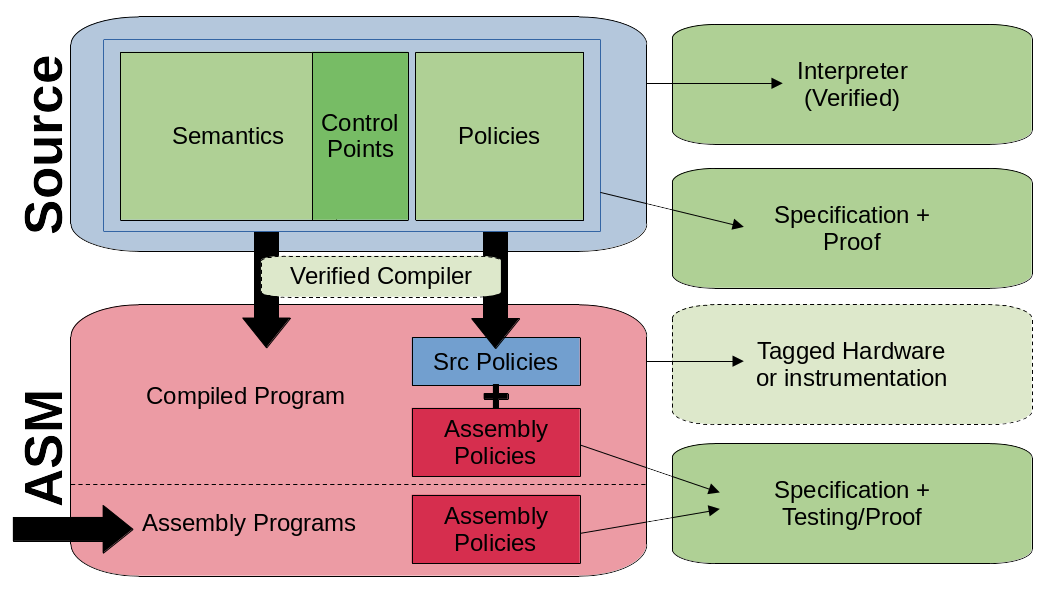
\includegraphics[width=\textwidth]{Structure.png}
  \caption{Tagging with Source Language}
  \label{fig:language}
\end{figure}

\section{Overview}

This dissertation is divided into three main parts. The first proposes a new formal characterization
of stack safety using concepts from language-based security. Stack safety exemplifies the challenges
of specifying a policy: ``the stack'' is not a clearly defined language concept, but a loosely
defined component of a system's ABI that is relied on by many different higher-level abstractions.
Performance tradeoffs are relevant as well: the ``lazy'' stack safety policies studied by
Roessler and DeHon~\cite{RoesslerD18} permit functions to write into one another's
frames, intuitively a violation, but taint the written locations so that their owner cannot
access them later. No prior characterization of stack safety captures this style of safety.

The second part presents Tagged C, a \emph{source-level} specification framework that allows
engineers to describe policies in terms of familiar C-level concepts. Tagged C addresses the
challenges in definition, specification, and validation that relate to assembly-level programs.
It takes the form of a variant C language whose semantics is parameterized by tags
attached to its data and rules that triggered during execution at a set of predefined
\emph{control points}. Control points correspond to significant execution events, such as
function calls, expression evaluation, and pointer-based memory accesses.

Tagged C allows policies to be defined at the source level via a fixed interface
that never requires rewriting code. Where assembly instructions can serve different roles and must
be distinguished for tag purposes, each Tagged C control point serves one clear role. The policy
designer needs little knowledge of how the control points might be compiled, and need not
deal with portions of a policy that would be colored red in Figure \ref{ex:call}.

The current iteration of Tagged C is implemented as an interpreter, based on that of
CompCert C \cite{Leroy09:CompCert}. This is sufficient to test small programs. Ultimately
Tagged C will be compiled to a PIPE target by injecting the source policy's tag rules
as a payload into a predefined assembly-level policy that handles the bookkeeping.

The Tagged-C semantics (also based on CompCert C) gives a formal definition of what each
control point does. This means that properties of a policy may be proven in terms of how
source programs behave when run under it. Just as it is far preferable to prove properties
of a program with respect to its source semantics, this is a major step forward for policy
verification. % Unclear

The final third of this dissertation makes use of Tagged C to perform a source-level specification and
verification of a novel compartmentalization property. The specification takes the form of
an abstract semantics that is compartmentalized by construction. This compartmentalized semantics
is written to keep compartments' local data isolated entirely in separate address spaces.
Both the specification and the policy that enforces it are novel, and improve upon the
state-of-the art in tag-based compartmentalization by allowing objects to be shared between
compartments via passed pointers, without the overhead of protecting every object individually.
The proof is mechanized. The policy definition, its
specification, and its proof are all concrete contributions on their own, and together they
serve to demonstrate that Tagged C is a suitable setting in which to perform the entire
define-specify-validate sequence.

\subsection{Contributions and Organization}

Chapter \ref{ch:background} introduces the concept of tag-based reference monitors
and brings the reader up to date on the state-of-the-art in that and related areas.
The contributions in this dissertation are divided across its three main topics.

\paragraph{Stack Safety}

Chapter \ref{ch:stacksafety} gives a novel formalization of stack safety in the
form of a collection of trace properties. Our contributions are:

\begin{itemize}
  \item A novel characterization of stack safety as a conjunction
        of security properties: confidentiality and integrity for callee
        and caller, plus well-bracketed control-flow.
        The properties are parameterized over a notion of
        external observation, allowing them to characterize lazy enforcement
        mechanisms.
  \item An extension of these core definitions to
        describe a realistic setting with argument passing on the stack,
        callee-saves registers, and tail-call elimination. The model is
        modular enough that adding these features is straightforward.
  \item Validation of a published enforcement mechanism,
        \emph{Lazy Tagging and Clearing}, via property-based random testing; we find that
        it falls short, and propose and validate a fix.
\end{itemize}

This chapter was first published at the IEEE Computer Security Foundations Symposium,
July 2023 as ``Formalizing Stack Safety as a Security Policy,'' a
joint work with Roberto Blanco, Leonidas Lampropoulos, Benjamin Pierce, and Andrew Tolmach
\cite{Anderson23:StackSafety}.

\paragraph{Tagged C}

In Chapter \ref{ch:taggedc}, we attack the definition problem by lifting tagged enforcement
to the level of C source code. We introduce Tagged C, a C variant whose semantics are parameterized
by an arbitrary tag-based policy. Our contributions are:

\begin{itemize}
\item The design of a comprehensive set of {\em control points} at which the C language interfaces
  with a tag-based policy. These expand on prior work by encompassing the full C language
  while being powerful enough to enable a range of policies even in the presence of C's more
  challenging constructs (e.g., {\tt goto}, conditional expressions, etc.).
\item Tagged C policies enforcing: (1) compartmentalization;
  (2) memory safety, with realistic memory models that support varying kinds of low-level idioms;
  and (3) secure information flow.
\item A full formal semantic definition for Tagged C, formalized in Coq, describing how the
  control points interact with programs, and an interpreter, implemented and verified against
  the semantics in Coq and extracted to OCaml.
\end{itemize}

The core of this chapter was first published at the International Conference on Runtime Verification,
October 2023 as ``Flexible Runtime Security Enforcement with Tagged C,'' a joint work
with Andrew Tolmach and Allison Naaktgeboren \cite{Anderson23:TaggedC}. Some technical
details are also published in Chhak et al. \cite{}, a joint work with CHR Chhak and Andrew Tolmach.
The original content has been updated to reflect further development, and the chapter has been
extended with a detailed discussion of the design decisions that inform the current development.

\paragraph{Compartmentalization}

Finally, I return to the specification and validation problems, now at the C level. Chapter
\ref{ch:compartments} presents a compartmentalization policy in conjunction with the abstract
compartmentalization scheme that it enforces, and proves that the policy indeed enforces the
abstract model. The detailed contributions are:

\begin{itemize}
\item A formal model of C compartmentalization in the form of an abstract machine that
  supports sharing between compartments while keeping their memories isolated by construction.
\item A novel compartmentalization policy for Tagged C that supports cross-compartment
  sharing with fewer constraints on available tags than similar systems from the literature.
\item A proof that the compartmentalization policy is safe with respect to the abstract semantics.
\end{itemize}

This work is not yet submitted for publication.

\chapter{Tags and Monitors}
\label{ch:background}

\chapter{Formalizing Stack Safety as a Security Policy}
\label{ch:stacksafety}

\chapter{Flexible Runtime Security Enforcement with Tagged C}
\label{ch:taggedc}

\chapter{Formalizing Compartmentalization as an Abstract Machine}
\label{ch:compartments}

\chapter{Conclusion}

\bibliographystyle{acm}
\bibliography{taggedc.bib}

\end{document}


\chapter{Tags and Monitors}
\label{ch:background}

\chapter{Formalizing Stack Safety as a Security Policy}
\label{ch:stacksafety}
\section{Introduction}
\label{ch3:sec:intro}

%\subsection{The Call Stack and Its Security}

Functions in high-level languages (and related abstractions such
as procedures, methods, etc.) are units of computation
that invoke one another to define larger computations in a modular way.
%
At a low level, each function activation manages its own local
variables, spilled temporaries, etc., as well as information about the
{caller} to which it will return.
%
The \emph{call stack} is the fundamental data structure used to
implement functions, aided by an Application Binary Interface (ABI)
that defines how registers are shared between activations.

From a security perspective, attacks on the call stack
are attacks on the function abstraction itself.
%
Indeed, the stack is an ancient~\cite{phrack96:smashingthestack} and
perennial~\cite{mitre-cwe,DBLP:conf/raid/VeendCB12,
  DBLP:conf/sp/SzekeresPWS13,
  DBLP:conf/sp/HuSACSL16,msrc-bluehat,chromium-security}
target for low-level attacks, sometimes involving control-flow
hijacking via corrupting the return address, sometimes memory corruption
more generally.
%
%The most recent release of the authoritative CWE Top 25
%Most Dangerous Software Weaknesses~\cite{
%list\footnote{\url{https://cwe.mitre.org/top25/archive/2022/2022_cwe_top25.html}}
%shows that general classes of vulnerabilities closely related to the stack
%% \rb{(though not exclusively)}
%consistently rank at and near the top of the list, e.g., \#1 Out-of-bounds Write, \#5 Out-of-bounds Read, and \#7 Use After Free.
%
%Moreover, many other types of faults involve some kind of control or data flow
%using data stored in the stack

The variety in attacks on the stack is mirrored in the range of
software and hardware protections that aim to prevent them,
%
including stack canaries~\cite{Cowan+98},
bounds checking~\cite{NagarakatteZMZ09,NagarakatteZMZ10,DeviettiBMZ08},
split stacks~\cite{Kuznetsov+14},
shadow stacks~\cite{Dang+15,Shanbhogue+19},
capabilities~\cite{Woodruff+14,Chisnall+15,SkorstengaardLocal,SkorstengaardSTKJFP,Georges22:TempsDesCerises},
and hardware tagging~\cite{DBLP:conf/sp/RoesslerD18,Gollapudi+23}.
%
But enforcement mechanisms can be brittle, successfully eliminating one
attack while leaving room for others. To avoid an endless game of
whack-a-mole, we seek formal properties of safe behavior that can be
proven, or at least rigorously tested. Such properties can be used as
the specification against which enforcement can be validated---even
enforcement mechanisms that do {\em not} fulfill a property can benefit from the
ability to articulate why and when they may fail.

Many of the mechanisms listed above are fundamentally ill-suited for
offering formal guarantees: they may impede attackers, but they do not provide
universal protection. Shadow stacks, for instance, aim to ``restrict
the flexibility available in creating gadget chains''
\cite{Shanbhogue+19}, not to categorically rule out attacks. Other
mechanisms, such as SoftBound~\cite{NagarakatteZMZ09} and code-pointer
integrity~\cite{Kuznetsov+14}, do aim for stronger guarantees, but not
formal ones.  To our knowledge, the sole
line of work making a formal claim to protect stack safety is the
study of secure calling conventions by Skorstengaard et
al.~\cite{SkorstengaardSTKJFP} and Georges et
al.~\cite{Georges22:TempsDesCerises}.

Some of the other mechanisms listed above should also be amenable to strong
formal guarantees.  In particular, Roessler and DeHon
\cite{DBLP:conf/sp/RoesslerD18} present an array of tag-based
micro-policies~\cite{pump_oakland2015} for stack safety that aim to offer
universal protection.  But the reasoning involved can be subtle:
they include micro-policy optimizations, Lazy Tagging and Lazy Clearing
(likely to be deployed together, which we hereafter refer to as Lazy
Tagging and Clearing, or LTC). LTC allows function activations to write
improperly into one another's stack frames, but ensures that the owner of
the corrupted memory cannot access it afterward, avoiding expensive
clearings of the stack frame.
%
Under this policy, one function activation {\em can} corrupt another's
memory---just not in ways that affect observable behavior.
Therefore, LTC would not fulfill Georges et al.'s property
(adapted to the tagged setting).  But LTC does arguably enforce stack safety,
or as Roessler and DeHon describe it informally, a sort of data-flow
integrity tied to the stack. A looser, more observational
definition of stack safety is needed to fit this situation.

We propose here a formal characterization of stack safety based on
the intuition of protecting function activations from each other and
using the tools of language-based
security~\cite{sabelfeld2003language} to treat function activations as
security principals.  We decompose stack safety into a family of
properties describing
the {\em integrity} and {\em confidentiality} of the caller’s local state
and the callee's behavior during (and after) the callee's execution,
together with the
{\em well-bracketed control flow} (\(\wbcf\)) property articulated by
Skorstengaard et al.~\cite{SkorstengaardSTKJFP}.

Our properties are stated abstractly in the hope that they can also be
applied to other enforcement mechanisms besides LTC.
%
However, it does not seem feasible to give
a universal definition of stack safety
that applies to all architectures and compilers.
While many security properties can be described purely at
the level of a high-level programming language and translated to a
target machine by a secure compiler, stack safety cannot be defined in
this way, since ``the stack'' is not explicitly present in the
definitions of most source languages but rather is implicit in the semantics
of features such as calls and returns.\footnote{
Contrast Azevedo de
  Amorim et al.'s work on heap safety
  \cite{DBLP:conf/post/AmorimHP18}, where the concept of the heap figures
  directly in high-level language semantics and its security is
  therefore amenable to a high-level treatment.}
%
But neither can stack safety be described coherently as a purely
low-level property;
indeed, at the lowest level, the specification of a ``well-behaved
stack'' is almost vacuous. The ISA is not concerned with such
questions as whether a caller's frame should be readable or writable
to its callee. Those are the purview of high-level languages built
atop the hardware stack.

Thus, any low-level treatment of stack safety must begin by asking:
which high-level features are supported in a given
setting using the stack, and how does their presence influence
the expectation of well-bracketed control flow, confidentiality,
and integrity? We begin with a simple system
with very few features, then move to a more realistic one supporting
tail-call elimination, argument passing on the stack, and callee-save
registers. Our properties are factored so that the basic structure
of each of our five properties remains constant while the presence or
absence of different features leads to subtler differences in how
they behave.

We demonstrate the usefulness of our properties for distinguishing
between correct and
incorrect enforcement using
QuickChick~\cite{Denes:VSL2014,Pierce:SF4}, a property-based
random testing tool for Coq.
Indeed, we find that the published version of LTC is flawed in
a way that undermines both integrity and confidentiality; after
correcting this flaw, LTC satisfies all of our
properties.  Further, we modify LTC to protect the features of
our more realistic system and apply
random testing to validate this extended protection mechanism against
the extended properties.

In summary, we offer the following contributions:

\begin{itemize}
\item We give a novel characterization of stack safety as a conjunction
  of security properties---confidentiality and integrity for callee
  and caller---plus well-bracketed control-flow.
  The properties are parameterized over a notion of
  external observation, allowing them to characterize lazy enforcement
  mechanisms.
\item We extend these core definitions to
  describe a realistic setting with argument passing on the stack,
  callee-saves registers, and tail-call elimination. The model is
  modular enough that adding these features is straightforward.
\item We validate a published enforcement mechanism, \emph{Lazy
  Tagging and Clearing}, via property-based random testing, find that
it falls short, and propose and validate a fix.
\end{itemize}
%
The following section offers a brief overview of our framework and
assumptions. \cref{ch3:sec:example} walks through a function call in
a simple example machine, discusses informally how each of our properties
applies to it, and motivates the properties
from a security perspective.
%
\cref{ch3:sec:formal} formalizes the machine model,
its {\em security semantics}, and the stack safety properties built on these.
\Cref{ch3:sec:extensions} describes how to support an extended set of features.
%\Cref{ch3:app:ptr} gives an (untested) proof-of-concept formalization of a more sophisticated,
%heap-like sharing model based on pointer provenance.
\Cref{ch3:sec:enforcement} describes the micro-policies that we test,
\cref{ch3:sec:testing} the testing framework itself, and
\cref{ch3:sec:relwork,sec:future} related and future work.

The accompanying artifact \footnote{https://github.com/SNoAnd/stack-safety}
contains formal definitions (in Coq) of our
properties, plus our testing framework.  It does not include proofs, since
we use Coq primarily for the QuickChick testing library and to
ensure that our definitions are unambiguous.  Formal proofs are left
as future work.

\section{Framework and Assumptions}
\label{ch3:sec:ideas}

Stack safety properties need to describe the behavior of machine code, but they naturally
talk about function activations and stack contents---abstractions that
are typically not visible at machine level. To bridge this gap,
our properties are defined in terms of a {\em security semantics} layered on top of
the standard execution semantics of the machine.  The security semantics identifies certain
state transitions of the machine as {\em security-relevant operations}, which update
a notional {\em security context}.  This context consists of
an (abstract) stack of function activations, each associated with a {\em view}
that maps each machine {\em state element} (memory location or register)
to a {\em security class} (active, sealed, etc.) specifying how the activation
can access the element.
The action of a security-relevant operation on the context is defined by a function
that characterizes how the operation's underling machine code ought to
implement the function abstraction in terms of the stack and registers.

Given the security classes of the elements of the machine state, we
define high-level
security properties---integrity, confidentiality, and well-bracketed
control flow---as
predicates that must hold on each call. These predicates draw on the idea of
\emph{variant} states from the theory of non-interference, plus a notion of
{\em observable events}, which might include specific function calls (e.g., system
calls that perform I/O), writes to special addresses representing
memory-mapped regions, etc. For example, to show that certain locations are kept
secret, it suffices to compare executions starting at machine states which vary at those locations
and check that their traces of observable events are the same. This structure
allows us to talk about the eventual impact of leaks or memory corruption without
reference to internal implementation details and, in particular, to support lazy enforcement by
flagging corruption of values only when it can actually impact visible behavior.

We introduce these properties by example in \cref{ch3:sec:example} and
formally in \cref{ch3:sec:formal}. In the remainder
of this section we introduce the underlying semantic framework
in more detail.

\paragraph*{Machine Model}
We assume a conventional ISA (e.g., RISC-V, x86-64, etc.), with registers including a program counter
and stack pointer.
%, and a standard ABI.
%\sna{Not in our formalism (hardcoded +4 in the definition of WBCF notwithstanding.)
%  This assumption is made in our example and testing.}
We make no particular assumptions about the provenance of the machine code; in particular,
we do not assume any particular compiler.
If the machine is enhanced with % security
enforcement mechanisms such as hardware
tags~\cite{pump_hasp2014,Gollapudi+23} or
capabilities~\cite{Woodruff+14}, we
assume that the behavior of these mechanisms is incorporated into the basic
step semantics of the machine, with a notion of ``compatible'' states that
share security behavior that may be defined based on the enforcement mechanism.
Failstop behavior by enforcement mechanisms is modeled as stepping to the same state
(and thus silently diverging).
%% \sna{I think that the payload concept is too nitty-gritty for this section.
%%   The chief use of the payload is that it allows every value to be interpreted
%%   as an address. In the tag world, it happens to coincide with a natural instance
%%   of our variant-compatibility relation.}

\paragraph*{Security Semantics}
A security semantics extends the core machine model
with additional context about the identities of current and pending
functions (which act as security principals) and about their security
requirements on registers and memory. This added context is purely notional;
it does not affect the behavior of the core machine. The security context
evolves dynamically through the execution of security-relevant operations,
which include calls, returns, and frame manipulation.
Our security properties are phrased in terms of this context, often as predicates
on future states (``when control returns to the current function, X
must hold...'')
or as relations on traces of future execution
(hyper-properties).

Security-relevant operations abstract over the implementation details of the
actions they take. Since the same machine instruction may be used by compilers for
different purposes, we assume that the compiler or another trusted
source has provided
labels to identify the security-relevant purpose of each instruction,
if any. For instance,
in the tagged RISC-V architecture
that we use in our examples and tests,
calls and returns are conventionally performed using the {\tt jal}
(``jump-and-link'')
and {\tt jalr} (``jump-and-link-register'') instructions, but these
instructions might also be used for other things.

These considerations lead to an annotated version of the
machine transition function, written \(\mach \xrightarrow{\bar{\psi},
  \obs} \mach'\), where \(\mach\) and \(\mach\) are machine states, \(\obs\) is
an optional externally observable event, and \(\overline{\psi}\) is a
list of security-relevant operations---necessary because a single step might
perform multiple simultaneous operations.
%
This is then lifted into a transition between pairs of machine states
and contexts by applying a transition function parameterized by the operation.
We will decompose this function into rules associated with each operation and introduce
them as needed.
%
The most important of these rules describe call and return operations.
A call pushes a new view onto the context stack and changes the class of the
caller's data to protect it from the new callee; a return reverses these steps.
Other operations signal how parts of the stack frame are being used to store
or share data, and their corresponding rules alter the classes of different
state elements accordingly.

Exactly which operations and rules are needed depends on
what code features we wish to support.
The set of security-relevant operations (\(\Psi\)) covered in this paper is given in
\cref{ch3:tab:psi}. A core set of operations covering calls, returns, and local
memory is introduced in the example in \cref{ch3:sec:example}
and formalized in \cref{ch3:sec:formal}. An extended set covering simple memory sharing and
tail-call elimination is described in \cref{ch3:sec:extensions} and tested in \cref{ch3:sec:testing}.
The remaining operations are needed for the capability-based model in
\cref{ch3:app:ptr}.

\newcommand{\example}{\rowcolor{black!0}}
\newcommand{\testing}{\rowcolor{black!10}}
\newcommand{\theory}{\rowcolor{black!25}}

\begin{table}
\begin{center}
  \begin{tabular}{| l | l | l |}
    \hline
    Operation \(\psi \in \Psi\) & Parameters & Sections\\
    \hline
    \example \(\mathbf{call}\) & target address, argument registers & \ref{ch3:sec:example},\ref{ch3:sec:formal}\\
    \testing & stack arguments (base, offset \& size) & \ref{ch3:sec:extensions},\ref{ch3:sec:testing} \\
    \example \(\mathbf{return}\) & & \ref{ch3:sec:example},\ref{ch3:sec:formal}\\
    \example \(\mathbf{alloc}\) & offset \& size & \ref{ch3:sec:example},\ref{ch3:sec:formal}\\
    \testing & public flag & \ref{ch3:sec:extensions},\ref{ch3:sec:testing} \\
    \example \(\mathbf{dealloc}\) & offset \& size &  \ref{ch3:sec:example},\ref{ch3:sec:formal}\\
    \testing \(\mathbf{tail call}\) & (same as for \(\mathbf{call}\)) & \ref{ch3:sec:extensions},\ref{ch3:sec:testing} \\
%    \hline
%    \multicolumn{2}{|c|}{{\it Pointer provenance operations}} \\
%    \hline
    \theory \(\mathbf{promote}\) & register, offset \& size & \ref{ch3:app:ptr} \\
    \theory \(\mathbf{propagate}\) & source register/address & \ref{ch3:app:ptr} \\
    \theory & destination register/address & \ref{ch3:app:ptr} \\
    \theory \(\mathbf{clear}\) & target register/address & \ref{ch3:app:ptr} \\
    \hline
  \end{tabular}
\end{center}
\caption{Security-relevant operations and their parameters, with the
  sections where they are first defined or used. Entries in light grey do not appear in
  our examples, but are part of our testing. Dark grey entries are not tested.}
\label{ch3:tab:psi}
\end{table}

\paragraph*{Views and Security Classes}

The security context consists of a stack of \emph{views}, where a view is a
function mapping
each state element to a {\it security class}---one of
\(\public\), \(\unsealed\), \(\object\), or \(\sealed\).

State elements that are outside of the stack---general-purpose memory used for
globals and the heap, as well as the code region and globally shared
registers---are always labeled \(\public\). We place security requirements on some
\(\public\) elements for purposes of the well-bracketed control flow \(\wbcf\) property, and a
given enforcement mechanism
might restrict their access (e.g., by rendering code immutable), but for integrity
and confidentiality purposes they are considered accessible at all times.

When a function is newly activated, every stack location that is available
for use but not yet initialized
is \(\unsealed\). From the perspective of the caller, the callee has no obligations
regarding its use of free elements.

Arguments are marked \(\object\), meaning that their contents may be
used safely.
When a function allocates memory for its own stack frame, that memory will also be \(\object\).
Then, on a call, \(\object\) elements that are not being used to communicate with
the callee will become \(\sealed\)---i.e., reserved for an inactive principal
and expected to be unchanged when it becomes active again.

\paragraph*{Instantiating the Framework}

Conceptually, the following steps are needed to instantiate the framework to a specific machine
and coding conventions: (i) define the base machine semantics, including any hardware
security enforcement features; (ii) identify the set of
security-relevant operations and rules required by the coding conventions; (iii) determine
how to label machine instructions with security-relevant
operations as appropriate; (iv) specify the form of observable events.

\paragraph*{Threat Model and Limitations}

When our properties are used to evaluate a system, the threat model
will depend on the details of that system. However, there are some
constraints that our design puts on any system. In particular, we must
trust that the security-relevant operations have been correctly labeled.
If a compiled function
call is not marked as such, then the caller's data might not be
protected from the callee; conversely, marking too many operations as
calls may cause otherwise safe programs to be rejected.

We do not assume that low-level code adheres to any single calling
convention or is being used to implement any particular
source-language constructs.
Indeed, if the source language is C, then high-level programs might
contain undefined behavior, in which case they might be compiled to
arbitrary machine code.

%tend to assume
%implicitly that callee-saved registers have their values maintained by whichever compiler
%generated their code. \apt{I do not understand the last sentence. Implementations of what?}
%Our properties explicitly state this as a requirement,
%which could be enforced by a micro-policy, a well-behaved compiler, or other enforcement technique.

In general, it is impossible to distinguish buggy machine code from an
attacker.  In examples, we often identify one function or another as
an attacker, but our framework does not require any static division between trusted
and untrusted code, and we aim to protect even buggy code.

This is a strong threat model, but it does omit some important aspects
of stack safety in real systems: in particular, it does not address
concurrency.  Hardware and timing attacks are also out of scope.
%

\section{Properties by Example}
\label{ch3:sec:example}

In this section, we introduce our security properties by means
of small code examples, using a simple set of security-relevant operations for
calls, returns, and private allocations.

\Cref{ch3:fig:main} gives C code and possible corresponding compiled 64-bit RISC-V code
for a function {\tt main}, which
takes an argument {\tt secret} and initializes a local variable {\tt sensitive} to contain
potentially sensitive data.
Then {\tt main} calls another function {\tt f},
and afterward it performs a test on {\tt sensitive} to decide whether
to output {\tt secret}.  Since {\tt sensitive} is initialized to 0,
the test should always fail, and {\tt main} should instead output the return value of {\tt f}.
Output is performed by writing to the special global {\tt out},
and we assume that such writes are the only observable events in the system.

The C code is compiled using the standard RISC-V calling conventions~\cite{RISC-V-CC}.
In particular, the function's first argument and its
return value are both passed in {\tt a0}.
Memory is byte addressed, and the stack grows towards
lower addresses. We assume that {\tt main} begins at address 0 and its
callee {\tt f} at address 100. The annotations in the right-hand column are
security-relevant operations, described further below.
The assembly is a simplified but otherwise typical compilation of the
source code into RISC-V; its details are less important than the positions
of the security-relevant operations.

\begin{figure}
  
  \newcommand{\figonebox}[1][]{\genbox{30pt}{blue!20}{#1}}
  \begin{subfigure}{0.49\textwidth}
    \small
    {\tt
      volatile int out;

      void main(int secret) \{

      ~ ~ int sensitive = 0;

      ~ ~ int res = f();

      ~ ~ if (sensitive == 42)

      ~ ~ ~ ~ out = secret;

      ~ ~ else

      ~ ~ ~ ~ out = res;

      \}}

    \vspace{\abovedisplayskip}
    \(\xleftarrow{\figonebox[\dots] \stackrel{\textsc{\normalsize sp}}{\figonebox[\tt res]}
    \stackrel{\textsc{\normalsize 4(sp)}}{\figonebox[\tt sens]}
    \stackrel{\textsc{\normalsize 8(sp)}}{\figonebox[\tt sec]}
    \stackrel{\textsc{\normalsize 12(sp)} \hfill}{\figonebox[\(\mathtt{ra_1}\)]\figonebox[\(\mathtt{ra_2}\)]}}\)

  \end{subfigure}
  \begin{subfigure}{0.5\textwidth}
    \small
    \begin{tabular}{r l | l}
      \labeledrow{0:}{addi sp,sp,-20}{\(\mathbf{alloc} ~ (-20,20)\)}
      \labeledrow{4:}{sd ra,12(sp)}{}
      \labeledrow{8:}{sw a0,8(sp)}{}
      \labeledrow{12:}{sw zero,4(sp)}{}
      \labeledrow{16:}{jal f,ra}{\(\mathbf{call} ~ \emplist \)}
      \labeledrow{20:}{sw a0,0(sp)}{}
      \labeledrow{24:}{lw a4,4(sp)}{}
      \labeledrow{28:}{li a5,42}{}
      \labeledrow{32:}{bne a4,a5,L1}{}
      \labeledrow{36:}{lw a0,8(sp)}{}
      \labeledrow{40:}{sw a0,out}{}
      \labeledrow{44:}{j L2}{}
      \labeledrow{L1, 48:}{lw a0,0(sp)}{}
      \labeledrow{52:}{sw a0,out}{}
      \labeledrow{L2, 56:}{ld ra,12(sp)}{}
      \labeledrow{60:}{addi sp,sp,20}{\(\mathbf{dealloc} ~ (0,20)\)}
      \labeledrow{64:}{jalr ra}{\(\mathbf{return}\)}
    \end{tabular}
  \end{subfigure}

  \caption{Example: C and assembly code for {\tt main} and layout of its stack frame (the stack grows to the left).}
  \label{ch3:fig:main}
\end{figure}

Now, suppose that {\tt f} is actually an attacker seeking
to leak {\tt secret}. It might do so in a number of ways, shown as snippets of
assembly code in \cref{ch3:fig:f}.
%
Leakage is most obviously viewed as a violation of {\tt main}'s {\it confidentiality}.
In \cref{ch3:subfig:direct}, {\tt f} takes an offset from the stack
pointer, accesses {\tt secret}, and directly outputs it.  More
subtly, even if it is somehow prevented from outputting {\tt secret}
directly, {\tt f}
can instead return its value so that {\tt main} stores it to {\tt out},
as in \cref{ch3:subfig:indirect}.
%
Beyond simply reading {\tt secret}, the attacker might overwrite {\tt sensitive}
with 42, guaranteeing that {\tt main} publishes its own secret unintentionally
(\cref{ch3:subfig:integrity}); this does not violate {\tt main}'s
confidentiality, but
rather its {\it integrity}.
In \cref{ch3:subfig:WBCF}, the attacker arranges to return to the
wrong instruction, thereby bypassing the check and publishing {\tt
  secret} regardless; this
violates the program's {\it well-bracketed control flow} (\(\wbcf\)).
%
In \cref{ch3:subfig:WBCF2}, a different attack violates \(\wbcf\), this time
by returning to the correct program counter but with the wrong stack pointer.
%
(We pad some of these variants with {\tt nop}s just so that all the
snippets have the same length, which keeps the step numbering uniform in~\cref{ch3:fig:exec1}.)

\begin{figure}
  \small
  \begin{subfigure}[b]{0.49\textwidth}
    \vspace{\abovedisplayskip}
    \begin{tabular}{r l | l}
      \labeledrow{100:}{lw a4,8(sp)}{}
      \labeledrow{104:}{sw a4,out}{}
      \labeledrow{108:}{li a0,1}{}
      \labeledrow{112:}{jalr ra}{\(\mathbf{return}\)}
    \end{tabular}
    \caption{Leaking {\tt secret} directly}
    \label{ch3:subfig:direct}
  \end{subfigure}
  \begin{subfigure}[b]{0.49\textwidth}
    \vspace{\abovedisplayskip}
    \begin{tabular}{r l | l}
      \labeledrow{100:}{lw a4,8(sp)}{}
      \labeledrow{104:}{mov a0,a4}{}
      \labeledrow{108:}{nop}{}
      \labeledrow{112:}{jalr ra}{\(\mathbf{return}\)}
    \end{tabular}
    \caption{Leaking {\tt secret} indirectly}
    \label{ch3:subfig:indirect}
  \end{subfigure}
  \begin{subfigure}[b]{0.49\textwidth}
    \vspace{\abovedisplayskip}
    \begin{tabular}{r l | l}
      \labeledrow{100:}{li a5,42}{}
      \labeledrow{104:}{sw a5,4(sp)}{}
      \labeledrow{108:}{li a0,1}{}
      \labeledrow{112:}{jalr ra}{\(\mathbf{return}\)}
    \end{tabular}
    \subcaption{Attacking {\tt sensitive}}
    \label{ch3:subfig:integrity}
  \end{subfigure}
  \begin{subfigure}[b]{0.49\textwidth}
    \vspace{\abovedisplayskip}
    \begin{tabular}{r l | l}
      \labeledrow{100:}{addi ra,ra,16}{}
      \labeledrow{104:}{nop}{}
      \labeledrow{108:}{nop}{}
      \labeledrow{112:}{jalr ra}{\(\mathbf{return}\)}
    \end{tabular}
    \subcaption{Attacking control flow}
    \label{ch3:subfig:WBCF}
  \end{subfigure}
  \begin{subfigure}[b]{\columnwidth}
    \vspace{\abovedisplayskip}
    \center
    \begin{tabular}{r l | l}
      \labeledrow{100:}{addi sp,sp,8}{}
      \labeledrow{104:}{nop}{}
      \labeledrow{108:}{nop}{}
      \labeledrow{112:}{jalr ra}{\(\mathbf{return}\)}
    \end{tabular}
    \subcaption{Attacking stack pointer integrity}
    \label{ch3:subfig:WBCF2}
  \end{subfigure}

  \caption{Example: assembly code alternatives for {\tt f} as an attacker.}
  \label{ch3:fig:f}
\end{figure}

The security semantics for this program is based
on the security-relevant events noted in the right columns of \cref{ch3:fig:main,fig:f},
namely execution of instructions that allocate or deallocate space (specified by
an \(\SP\)-relative offset and size), make a call (with a specified list of argument registers),
or make a return.

Our security semantics attaches a security context to the machine state,
consisting of a view \(V\) and a stack \(\sigma\) of pending activations' views.
\Cref{ch3:fig:exec1} shows how the security context evolves over the first few
steps of the program.  (The formal details of the security semantics are described in
\cref{ch3:sec:formal}, and the context evolution rules are formalized in \cref{ch3:fig:basicops}.)
Execution begins at the start of {\tt main}, with the program counter
(\(\PCname\)) set to zero and the stack pointer (\(\SP\)) at address 1000.
State transitions are numbered and may be labeled with a security operation, written
\(\downarrow \psi\), between steps.

The initial view \(V_0\) maps all stack addresses below \(\SP\) to \(\unsealed\) and the remainder of
memory to \(\public\). The sole used argument register, {\tt a0}, is mapped to \(\object\);
other caller-save registers are mapped to \(\unsealed\) and callee-save registers to \(\sealed\).
Step 1 allocates a word each for {\tt secret}, {\tt sensitive}, and {\tt res}, as well
as two words for the return address; this has the
effect of marking those bytes \(\object\).
We use \(V\llbracket\ldots\rrbracket\) to denote updates to \(V\).

\begin{figure*}
  \scriptsize
  \begin{tabular}{|r|r||l|r}
    \cline{1-3}
    \(\PCname\) & \(\SP\) & Context &
    \multirow{3}{*}{\(\underbrace{\dots \freebox \freebox \freebox \freebox \freebox
        \freebox \freebox \freebox \freebox \freebox}_\unsealed
      \! \underbrace{\stackrel{\stackrel{\SP}{\downarrow}}{\pubbox} \!\! \pubbox \pubbox \dots}_\public
      ~ \stackrel{\mathtt{a0}}{\objbox\objbox} ~ \stackrel{\mathtt{a4}}{\freebox\freebox}
      ~ \stackrel{\mathtt{a5}}{\freebox\freebox}
      \)} \\
    \cline{1-3}
    0 & 1000 & \(V_0, \emplist\)
    \\
    \cline{1-3}
    \multicolumn{3}{l}{\multirow{2}{*}{\(1 \Big\downarrow \mathbf{alloc} ~ (-20,20)\)}} & \\
    \multicolumn{3}{l}{} &
    \multirow{3}{*}{\(\underbrace{\dots \freebox \freebox \freebox \freebox \freebox}_\unsealed
      \! \underbrace{\stackrel{\stackrel{\SP}{\downarrow}}{\objbox} \!\! \objbox \objbox \objbox \objbox}_\object
      \! \underbrace{\pubbox \pubbox \pubbox \dots}_\public
      ~ \stackrel{\mathtt{a0}}{\objbox\objbox} ~ \stackrel{\mathtt{a4}}{\freebox\freebox}
      ~ \stackrel{\mathtt{a5}}{\freebox\freebox}
      \)}
    \\
    \cline{1-3}
    4 & 980 & \(V_1 = V_0 \llbracket 980..999 \mapsto \object\rrbracket, \emplist\) &
    \\
    \cline{1-3}
    \multicolumn{3}{l}{\multirow{2}{*}{2-4 \(\Big\downarrow\)}} \\ \multicolumn{3}{l}{} \\
    \cline{1-3}
    16 & 980 & \(V_1, \emplist\) & \\
    \cline{1-3}
    \multicolumn{3}{l}{\multirow{2}{*}{\(5 \Big\downarrow \mathbf{call} ~ 100 ~ \emplist\)}} & \\
    \multicolumn{3}{l}{} &
    \multirow{3}{*}{\(\underbrace{\dots \freebox \freebox \freebox \freebox \freebox}_\unsealed
      \! \underbrace{\stackrel{\stackrel{\SP}{\downarrow}}{\sealbox} \!\! \sealbox \sealbox \sealbox \sealbox}_\sealed
      \! \underbrace{\pubbox \pubbox \pubbox \dots}_\public
      ~ \stackrel{\mathtt{a0}}{\freebox\freebox} ~ \stackrel{\mathtt{a4}}{\freebox\freebox}
      ~ \stackrel{\mathtt{a5}}{\freebox\freebox}
      \)}
    \\
    \cline{1-3}
    100 & 980 & \(V_2 = V_1 \left\llbracket \begin{tabular}{l}
      \(980..999 \mapsto \sealed,\) \\
      \(\mathtt{a0} \mapsto \unsealed\) \\ \end{tabular} \right\rrbracket,[V_1]\) & \\
    \cline{1-3}
    \multicolumn{3}{l}{\multirow{2}{*}{6-8 \(\Big\downarrow\)}} \\ \multicolumn{3}{l}{} \\
    \cline{1-3}
    112 & 980 & \(V_2,[V_1]\) \\
    \cline{1-3}
    \multicolumn{3}{l}{\multirow{2}{*}{\(9 \Big\downarrow \mathbf{return}\)}} & \\
    \multicolumn{3}{l}{} & \multirow{3}{*}{\(\underbrace{\dots \freebox \freebox \freebox \freebox \freebox}_\unsealed
      \! \underbrace{\stackrel{\stackrel{\SP}{\downarrow}}{\objbox} \!\! \objbox \objbox \objbox \objbox}_\object
      \! \underbrace{\pubbox \pubbox \pubbox \dots}_\public
      ~ \stackrel{\mathtt{a0}}{\objbox\objbox} ~ \stackrel{\mathtt{a4}}{\freebox\freebox}
      ~ \stackrel{\mathtt{a5}}{\freebox\freebox}
      \)}
    \\
    \cline{1-3}
    20 & 980  & \(V_1, \emplist\) &
    \\
    \cline{1-3}
    \multicolumn{2}{l}{} \\
  \end{tabular}
  \caption{Execution of example up through the return from {\tt f}. In stack diagrams, addresses increase to the right, stack grows to the left, and boxes represent 4-byte words.}
\label{ch3:fig:exec1}
\end{figure*}
%
At step 5, the current principal's record is pushed onto the inactive list.
The callee's view is updated from the caller's such that all \(\object\) memory locations
become \(\sealed\). (For now we assume no sharing of stack memory between activations; data is
passed only through argument registers, which remain active. In the presence of memory
sharing, some memory would remain active, too.)
Function {\tt f} does not take any arguments; if it did, any registers containing them would be
mapped to \(\object\), while any non-argument, caller-saved
registers are mapped to \(\unsealed\). In the current example, only register {\tt a0}  changes
security class. All callee-save registers remain \(\sealed\) for all calls, so
if, in the example, we varied the assembly code for {\tt main} so that {\tt sensitive} was stored
in a callee-save register (e.g., {\tt s0}) rather than in memory, its security class would still
be \(\sealed\) at the entry to {\tt f}.
%
At step 9, {\tt f} returns and the topmost inactive view, that of {\tt main}, is restored.

We now show how this security semantics can be used to define notions of confidentiality,
integrity, and correct control flow in such a way that many classes of
bad behavior, including the attacks in \cref{ch3:fig:f}, are
detected as security violations.

\paragraph*{Well-Bracketed Control Flow}

To begin with, if {\tt f} returns to an unexpected place (i.e., \(\PCname \neq 20\) or
\(\SP \neq 980\)), we say that it has violated \(\wbcf\). \(\wbcf\) is a relationship between
call steps and their corresponding return steps: just after the return, the program
counter should be at the next instruction below the call,
and the stack pointer should have the same value that it had before the call.
Both of these are essential for security. In \cref{ch3:subfig:WBCF}, the attacker adds
16 to the return address and then returns; this bypasses the {\tt if}-test in the code and outputs
{\tt secret}.
In \cref{ch3:subfig:WBCF2}, the attacker returns with \(\SP' = 988\) instead of the
correct \(\SP = 980\). In this scenario, given the layout of {\tt main}'s frame,
\begin{center}
\begin{tabular}{| l | l | l | l | l |}
  \multicolumn{1}{r}{\(\SP \downarrow\)} &
  \multicolumn{2}{r}{\(\SP' \downarrow\)} \\
  \hline
  {\tt res} & {\tt sens} & {\tt sec} & \(\mbox{\tt ra}_1\) & \(\mbox{\tt ra}_2\) \\
  \hline
\end{tabular}
\end{center}

\vspace{\abovedisplayskip}

\noindent
{\tt main}'s attempt to read {\tt sensitive} may instead
read part of the return address, and its attempt to output
{\tt res} will instead output {\tt secret}.

Before the call, the program counter is 16 and the stack pointer is 980.
So we define a predicate on states that should hold just after the return:
\(\ret\ \mach \triangleq \mach[\PCname] = 20 \wedge \mach[\SP] = 980\).
%
We can identify the point just after the return (if a return occurs)
as the first state in which the pending call stack is smaller than it was
just after the call.
\(\wbcf\) requires that, if \(\mach\) is the state at that point, then \(\ret ~ \mach\) holds.
This property is formalized in \cref{ch3:tab:props}, line 1.
%For nested calls, where the pending stack is initially larger, the same principle
%applies: \(\ret ~ \mach\) must hold the next time the pending stack is the same size or smaller.

% Even absent other
% kinds of data protection, the stack pointer {\it must} be restored
% for the program to behave predictably.

\paragraph*{Stack Integrity}

Like \(\wbcf\), stack integrity defines a condition at the call that must hold upon
return. This time the condition applies to all of the memory in the caller's
frame. In \cref{ch3:fig:exec1} we see the lifecycle of an allocated frame:
upon allocation, the view labels it \(\object\), and when a call is made, it instead
becomes \(\sealed\). Intuitively, the integrity of {\tt main}
is preserved if, when control returns to it, any \(\sealed\) elements
are identical to when it made the call.
%
Again, we need to know when a caller has been returned to,
and we use the same mechanism of checking the depth of the call stack.
%
In the case of the call from {\tt main} to {\tt f}, the \(\sealed\) elements are the
addresses 980 through 999 and callee-saved registers such as
the stack pointer. Note that callee-saved registers often change
during the call---but if the caller accesses them after the call, it should find them
restored to their prior value.

While it would be simple to define integrity as ``all sealed elements retain their
values after the call,'' this would be stricter than necessary. Suppose that
a callee overwrites some data of its caller, but the caller never accesses that data
(or only does so after re-initializing it). This would be harmless, with the callee
essentially using the caller's memory as scratch space, but the caller never seeing any change.

For a set of elements \(\components\),
a pair of states \(\mach\) and \(\nach\) are {\em \(\components\)-variants} if
their values an only disagree on elements in \(\components\).
We say that the elements of \(\components\) are \emph{irrelevant}
in \(\mach\) if they can be replaced by arbitrary other values without changing the
observable behavior of the machine. All other elements are \emph{relevant}.\footnote{
This story is slightly over-simplified. If an enforcement mechanism maintains
additional state associated with elements, such as tags, we don't want that
state to vary. This is touched on in \cref{ch3:sec:props}.
}

We define \emph{caller integrity} (\(\clri\))  as the property that
every relevant element that is \(\sealed\) under the callee's view is restored
to its original value at the return point.
(This property is formalized in \cref{ch3:tab:props}, line 2).

\newcommand{\figfourbox}[1][]{\genbox{20pt}{red}{#1}}

\begin{figure}
  \scriptsize
  \centering
  \[
  \stackrel{\texttt{res}}{\figfourbox[0]}
  \stackrel{\texttt{sens}}{\figfourbox[0]}
  \stackrel{\texttt{sec}}{\figfourbox[5]}
  \stackrel{\texttt{ra}}{\figfourbox[0]\figfourbox[0]}\]
  %
  \[\big\Downarrow\]
  %
  \[
  \stackrel{\texttt{res}}{\figfourbox[0]}
  \stackrel{\texttt{sens}}{\genbox{20pt}{red!50}{\bf 42}}
  \stackrel{\texttt{sec}}{\figfourbox[5]}
  \stackrel{\texttt{ra}}{\figfourbox[0]\figfourbox[0]}\]
  %
  \[\overbrace{
    \stackrel{\texttt{res}}{\figfourbox[0]}
    \stackrel{\texttt{sens}}{\genbox{20pt}{\leftvariant}{\bf 42}}
    \stackrel{\texttt{sec}}{\figfourbox[5]}
    \stackrel{\texttt{ra}}{\figfourbox[0]\figfourbox[0]}
    \hspace{1cm}
    \stackrel{\texttt{res}}{\figfourbox[0]}
    \stackrel{\texttt{sens}}{\genbox{20pt}{\rightvariant}{\bf 0}}
    \stackrel{\texttt{sec}}{\figfourbox[5]}
    \stackrel{\texttt{ra}}{\figfourbox[0]\figfourbox[0]}}\]
  \[\stackrel{\hookrightarrow \mathtt{out}}{\genbox{20pt}{white}{5}} \hspace{0.5cm}
  %\raisebox{\height}{\not\approx}
  \hspace{0.5cm}
  \stackrel{\hookrightarrow \mathtt{out}}{\genbox{20pt}{white}{1}}\]
  \caption{Integrity Violation: {\tt sensitive} changed, and if varied, changes future outputs}
  \label{ch3:fig:variant}
\end{figure}

In our example setting, the observation trace consists of the sequence
of values written to {\tt out}. In \cref{ch3:subfig:integrity} the states before
and after the call differ in the value of {\tt sensitive}. \Cref{ch3:fig:variant}
shows the states before and after the call, which disagree on the value at
{\tt sensitive}. If we consider a
variant of the original return state in which {\tt sensitive} is 0 (orange)
as opposed to 42 (blue), that state will eventually output 1, while the actual
execution outputs 5. This means that {\tt sensitive} is relevant.

To be more explicit, similar to \(\wbcf\), we define
\(\intProp\) as a predicate on states that holds if
all relevant sealed addresses in \(\mach\) are the same as after step 5.
We require that \(\intProp\) hold on the state following the matching return,
which is reached by step 9. Here {\tt sensitive} has obviously changed, but we
just saw that it is relevant.

\paragraph*{Caller Confidentiality}

We treat confidentiality as a form of non-interference as well: the confidentiality of a caller
means that its callee's behavior is dependent only on publicly visible data,
not the caller's private state. This also requires that the callee initialize
memory before reading it.
As we saw in the examples, we must consider both the observable events
that the callee produces during the call and the changes that the callee makes to the state that might
affect the caller after the callee returns.

Consider the state after step 5, shown at the top of \cref{ch3:fig:variant2},
with the attacker code from \cref{ch3:subfig:direct} and the assumption that
{\tt secret} has the value 5. We take a variant state over
the set of elements that are \(\sealed\) in \(V_2\) (orange), and compare it to the
original (blue). During the execution, the value of {\tt secret} is written
to the output, and the information leak is evidenced by the fact that the
outputs do not agree---the original outputs 5, while the variant outputs 3.
This is a violation of
{\it internal confidentiality} (formalized in \cref{ch3:tab:props}, line 3a).

\newcommand{\leftbox}[1][]{\genbox{20pt}{\leftvariant}{#1}}
\newcommand{\rightbox}[1][]{\genbox{20pt}{\rightvariant}{#1}}

\begin{figure}
  \scriptsize
  \centering
    \[
    \stackrel{\texttt{res}}{\figfourbox[0]}
    \stackrel{\texttt{sens}}{\figfourbox[0]}
    \stackrel{\texttt{sec}}{\figfourbox[5]}
    \stackrel{\texttt{ra}}{\figfourbox[0]\figfourbox[0]}\]
    %
    \[\overbrace{
    \stackrel{\texttt{res}}{\leftbox[0]}
    \stackrel{\texttt{sens}}{\leftbox[0]}
    \stackrel{\texttt{sec}}{\leftbox[5]}
    \stackrel{\texttt{ra}}{\leftbox[0]\leftbox[0]}
    \hspace{1cm}
    %
    \stackrel{\texttt{res}}{\rightbox[1]}
    \stackrel{\texttt{sens}}{\rightbox[2]}
    \stackrel{\texttt{sec}}{\rightbox[3]}
    \stackrel{\texttt{ra}}{\rightbox[4]\rightbox[5]}}
    \]
    \[\raisebox{.5\height}{\Bigg\Downarrow} \hspace{1cm}
    \stackrel{\hookrightarrow \mathtt{out}}{\genbox{20pt}{white}{5}} \hspace{0.5cm}
    \raisebox{\height}{\(\not\approx\)}
    \hspace{0.5cm}
    \stackrel{\hookrightarrow \mathtt{out}}{\genbox{20pt}{white}{3}} \hspace{1cm}
    \raisebox{.5\height}{\Bigg\Downarrow}
    \]
    \[
    \stackrel{\texttt{res}}{\leftbox[0]}
    \stackrel{\texttt{sens}}{\leftbox[0]}
    \stackrel{\texttt{sec}}{\leftbox[5]}
    \stackrel{\texttt{ra}}{\leftbox[0]\leftbox[0]}
    \hspace{1cm}
    %
    \stackrel{\texttt{res}}{\rightbox[1]}
    \stackrel{\texttt{sens}}{\rightbox[2]}
    \stackrel{\texttt{sec}}{\rightbox[3]}
    \stackrel{\texttt{ra}}{\rightbox[4]\rightbox[5]}
    \]

  \caption{Internal Confidentiality Violation}
  \label{ch3:fig:variant2}
\end{figure}

But, in \cref{ch3:subfig:indirect}, we also saw an attacker that exfiltrated the secret
by reading it and then returning it, in a context where the caller would output the returned
value. \Cref{ch3:fig:variant3} shows the behavior of the same variants under this attacker,
but in this case, there is no output during the call. Instead the value of {\tt secret} is
extracted and placed in {\tt a0}, the return value register.
%
\begin{figure}
  \scriptsize
    \centering
    \[
    \stackrel{\texttt{res}}{\figfourbox[0]}
    \stackrel{\texttt{sens}}{\figfourbox[0]}
    \stackrel{\texttt{sec}}{\figfourbox[5]}
    \stackrel{\texttt{ra}}{\figfourbox[0]\figfourbox[0]}\]
    %
    \[\overbrace{
    \stackrel{\texttt{res}}{\leftbox[0]}
    \stackrel{\texttt{sens}}{\leftbox[0]}
    \stackrel{\texttt{sec}}{\leftbox[5]}
    \stackrel{\texttt{ra}}{\leftbox[0]\leftbox[0]}
    \hspace{1cm}
    %
    \stackrel{\texttt{res}}{\rightbox[1]}
    \stackrel{\texttt{sens}}{\rightbox[2]}
    \stackrel{\texttt{sec}}{\rightbox[3]}
    \stackrel{\texttt{ra}}{\rightbox[4]\rightbox[5]}}
    \]
    \[\raisebox{.5\height}{\Bigg\Downarrow} \hspace{1cm} \stackrel{\mathtt{a0}}{\leftbox[\bf 0]} \hspace{1cm}
    \stackrel{\mathtt{a0}}{\rightbox[\bf 6]} \hspace{1cm} \raisebox{.5\height}{\Bigg\Downarrow}\]
    \[
    \stackrel{\texttt{res}}{\leftbox[0]}
    \stackrel{\texttt{sens}}{\leftbox[0]}
    \stackrel{\texttt{sec}}{\leftbox[5]}
    \stackrel{\texttt{ra}}{\leftbox[0]\leftbox[0]}
    \hspace{1cm}
    %
    \stackrel{\texttt{res}}{\rightbox[1]}
    \stackrel{\texttt{sens}}{\rightbox[2]}
    \stackrel{\texttt{sec}}{\rightbox[3]}
    \stackrel{\texttt{ra}}{\rightbox[4]\rightbox[5]}
    \]
    \[\stackrel{\mathtt{a0}}{\leftbox[\bf 5]} \hspace{1cm}
    \stackrel{\mathtt{a0}}{\rightbox[\bf 3]}\]
  \caption{Return-time Confidentiality Violation}
  \label{ch3:fig:variant3}
\end{figure}

At the end of the call, we can deduce that every element on which
the variant states disagree must carry some information derived from
the original varied elements. In most cases, that is because the element
is one of the original varied elements and has not changed during the
call, which does not represent a leak. But in the case of {\tt a0}, it
has changed during the call, {\em and} the return states do not agree
on its value. This represents data that has been leaked, and should
not be used to affect future execution.
Unless {\tt a0} happens to be irrelevant to the caller, this example
is a violation of what we term {\it return-time confidentiality}
(formalized in \cref{ch3:tab:props}, line 3b).

Structurally, return-time confidentiality resembles integrity, but now dealing with
variants. We begin with a state immediately following
a call, \(\mach\). We consider an arbitrary variant state,
\(\nach\), which may vary any element that is \(\sealed\) or \(\unsealed\),
i.e., any element that is not used legitimately to pass arguments. Caller confidentiality
therefore can be thought of as the callee's insensitivity to elements in its initial state
that are not part of the caller-callee interface.

We define a binary relation \(\confProp\) on pairs of states,
which holds on eventual return states \(\mach'\) and \(\nach'\)
if all relevant elements are {\em uncorrupted} relative to \(\mach\) and \(\nach\).
An element is {\em corrupted} if it differs between \(\mach'\) and \(\nach'\),
and it either changed between \(\mach\) and \(\mach'\) or between \(\nach\) and \(\nach'\).

Finally, we define \emph{caller confidentiality} (\(\clrc\)) as the
combination of internal and return-time confidentiality (\cref{ch3:tab:props}, line 3).

\paragraph*{The Callee's Perspective}

We presented our initial example from the perspective of the caller, but a callee
may also have privilege that its caller lacks, and which must be protected from the
caller. Consider a function that makes a privileged system call to obtain a secret key,
and uses that key to perform a specific task. An untrustworthy or erroneous caller might
attempt to read the key out of the callee's memory after return, or to influence the callee
to cause it to misuse the key itself!

Where the caller's confidentiality and integrity are concerned with protecting specific,
identifiable state---the caller's stack frame---their callee equivalents are concerned
with enforcing the expected interface between caller and callee. Communication between
the principals should occur only through the state elements that are designated for the
purpose: those labeled \(\public\) and \(\object\).

Applying this intuition using our framework, \emph{callee confidentiality} (\(\clec\))
turns out to resemble \(\clri\), extended to every element that is not marked \(\object\)
or \(\public\) at call-time. The callee's internal behavior is represented by those
elements that change over the course of its execution, and which are not part of the
interface with the caller. At return, those elements should become irrelevant to the
subsequent behavior of the caller.

Similarly, in \emph{callee integrity} (\(\clei\)), only elements marked \(\object\)
or \(\public\) at the call should influence the behavior of the callee. It may seem
odd to call this integrity, as the callee does not have a private state. But
an erroneous callee that performs a read-before-write within its stack
frame, or which uses a non-argument register without initializing it, is vulnerable
to its caller seeding those elements with values that will change its behavior.
The fact that well-behaved callees have integrity by definition is probably why
callee integrity is not typically discussed.

\section{Formalization}
\label{ch3:sec:formal}

We now give a formal description of our machine model, security semantics,
and properties. Our definitions abstract over: (i) the details of  the target machine
architecture and ABI, (ii) the set of security-relevant operations and their effects on
the security context, (iii) the set of observable events, and (iv) a notion of value compatibility.

\subsection{Machine}
The building blocks of a machine are {\em words} and {\em registers}.
Words are ranged over by \(\word\) and, when used as addresses, \(\addr\),
and are drawn from the set \(\WORDS\).
Registers in the set \(\REGS\) are ranged over by \(\reg\), with the stack pointer
given the special name \(\SP\);
some registers may be classified as caller-saved (CLR) or callee-saved (CLE).
Along with the program counter, \(\PCname\), these are referred to as
{\em state elements} \(\component\) in the set \(\COMPONENTS ::= \PCname | \WORDS | \REGS\).

A {\em machine state} \(\mach \in \MACHS\) is a map from state elements to a set \(\mathcal{V}\) of
\emph{values}.
Each value \(v\) contains a \emph{payload} word, written \(|v|\).
We write \(\mach[\component]\) to denote the value of \(\mach\) at
\(\component\)  and \(\mach[v]\) as shorthand for \(\mach[|v|]\).
Depending on the specific machine being modeled, values may also contain other
information relevant to hardware enforcement (such as a tag).
%Intuitively, the payload represents the part of the value that is relevant to
%the behavior of the basic machine, and it is the part that should be changed
When constructing variants (see~\cref{ch3:sec:props}, this additional information should
not be varied. To capture this idea, we assume a given \emph{compatibility} equivalence relation \(\sim\) on values,
and lift it element-wise to states.  Two values should be compatible if their
non-payload information (e.g., their tag) is identical.
%% \apt{This is still not very convincing!
%%   empting to say that only the payloads can affect the step function, but that is
%%   too strong, right? (OK for tags, but not, e.g., capabilities?}
%% \sna{Yeah, I don't think we can say something universal about when values should be
%%   considered compatible.}

The machine has a step function \(\mach \xrightarrow{\bar{\psi},\obs} \mach'\).
Except for the annotations over the arrow, this function just encodes the usual
ISA description of the machine's instruction set. The annotations serve to connect
the machine's operation to our security setting:
\(\bar{\psi}\) is a list of security-relevant operations drawn from an assumed given set \(\Psi\),
and \(\obs\) is an (potentially silent) observable event; these are described further below.

\subsection{Security semantics}

The security semantics operates in parallel with the machine.
Each state element (memory word or register) is given a \emph{security class}
\(l \in \{\public, \object, \sealed, \unsealed\}\).
A \emph{view} \(V \in \mathit{VIEW}\) maps elements to security classes.
For any security class \(l\), we write \(l(V)\)
to denote the set of elements \(\component\) such that \(V ~ \component = l\).
The {\it initial view} \(V_0\) maps all stack locations to \(\unsealed\),
all other locations to \(\public\), and registers based on which set they
belong to: \(\sealed\) for callee-saved, \(\unsealed\) for caller-saved except for those
that contain arguments at the start of execution, which are \(\object\), and \(\public\) otherwise.

A (security) \emph{context} is
a pair of the current activation's view and
a list of views representing the call stack (pending inactive
principals), ranged over by \(\sigma\).
%
\[\context \in \CONTEXTS ::= \mathit{VIEW \times list ~ VIEW}\]
%
The initial context is \(\context_0 = (V_0, \emplist)\).

\Cref{ch3:sec:example} describes informally how the security context evolves as the system performs
security-relevant operations. Formally, we combine each machine state with a context
to create a {\it combined state} \(s = (\mach,\context)\) and lift the transition
to \(\stepstounder{}\) on combined states.
At each step, the context updates based on an assumed given function
\(Op : \MACHS \rightarrow \CONTEXTS \rightarrow \Psi \rightarrow \CONTEXTS\).
Since a single step might correspond to multiple operations, we apply
\(Op\) as many times as needed, using \(\mathit{foldl}\).

\judgmenttwo{\(\mach \xrightarrow{\overline{\psi},\obs} \mach' \)}
            {\(\mathit{foldl} ~ (Op ~ \mach) ~ \context ~ \overline{\psi} = \context'\)}
            {\((\mach,\context) \stepstounder{\overline{\psi},\obs} (\mach', \context')\)}

A definition of \(Op\) is most convenient to present decomposed into
rules for each operation. We have already seen the intuition behind the rules for
\(\mathbf{alloc}\), \(\mathbf{call}\), and \(\mathbf{ret}\).
For the machine described in the example, the \(Op\) rules would be those
found in \cref{ch3:fig:basicops}.
Note that \(Op\) takes as its first argument the state {\it before} the step.

\begin{figure}
  
  \[\mathit{range} ~ \reg ~ \mathit{off} ~ \mathit{sz} ~ \mach \triangleq
    \{\mach[\reg]+i | \mathit{off} \leq i < \mathit{off+sz}\}\]

    \judgmentbr[~Alloc]
               {\(\components = \mathit{range} ~ \SP ~ \mathit{off} ~ \mathit{sz} ~ \mach \cap \unsealed(V)\)}
               {\(V' = V \llbracket \addr \mapsto \object \mid \addr \in \components \rrbracket\)}
               {\(Op ~ \mach ~ (\mathbf{alloc} ~ \mathit{off, sz}) ~ (V,\sigma) = (V',\sigma)\)}
               
    \vspace{\abovedisplayskip}

    \judgmentbr[~Dealloc]
               {\(\components = \mathit{range}~ \SP ~ \mathit{off} ~ \mathit {sz} ~ \mach \cap \object(V)\)}
               {\(V' = V \llbracket \addr \mapsto \unsealed \mid \addr \in \components \rrbracket\)}
               {\(Op ~ \mach ~ (\mathbf{dealloc} ~ \mathit{off, sz}) ~ (V,\sigma) = (V',\sigma)\)}

    \vspace{\abovedisplayskip}
    
    \judgment[~Call]
             {\(V' = \lambda \component .
               \begin{cases}
                 \unsealed & \textnormal{if } k \in CLR \\
                 \public & \textnormal{if } k \in \overline{\reg_{\mathit{args}}} \\
                 \sealed & \textnormal{if } k \in \WORDS \textnormal{ and } k \in \object(V) \\
                 V(k) & \textnormal{otherwise} \\
               \end{cases}\)}
             {\(Op ~ \mach ~ (\mathbf{call} ~ \addr_{target} ~ \overline{\reg_{args}})
               ~ (V,\sigma) = (V',V::\sigma)\)}

    \vspace{\abovedisplayskip}             
    
    \judgment[~Return]
             {}
             {\(Op ~ \mach ~ \mathbf{return} ~ (\_, (V,\sigma')) = (V, \sigma')\)}
             \caption{Basic Operations}
  \label{ch3:fig:basicops}
\end{figure}

\subsection{Events and Traces}
\label{ch3:sec:events}

We abstract over the events that can be observed in the system, assuming just
a given set \(\OBSS\) that contains at least the element \(\tau\), the silent
event. Other events might represent certain function calls (i.e., system calls)
or writes to special addresses representing memory-mapped regions.
A {\em trace} is a nonempty, finite or infinite sequence
of events, ranged over by \(\obsT\).
We use ``\(\notfinished{}{}\)'' to represent ``cons'' for traces, reserving ``::''
for list-cons.

We are particularly interested in traces that end just after a function returns.
We define these in terms of the depth \(d\) of the security context's call stack \(\sigma\).
We write \(d \hookrightarrow s\) for the trace of execution from a state \(s\)
up to the first point where the stack depth is smaller than \(d\), defined
coinductively by these rules:

\judgment[~Done]
         {\(|\sigma| < d\)}
         {\(d \hookrightarrow (\mach,(V,\sigma)) = \tau\)}

\vspace{\abovedisplayskip}
         
\judgmenttwobrlong[~Step]
                  {\(|\sigma| \geq d\)}
                  {\(d \hookrightarrow (\mach',\context') = \obsT\)}
                  {\((\mach,(V,\sigma)) \stepstounder{\overline{\psi},\obs} (\mach',\context')\)}
                  {\(d \hookrightarrow (\mach,(V,\sigma)) = \notfinished{\obs}{\obsT}\)}

\noindent
When \(d = 0\), the trace will always be infinite because the machine never halts; in this case we
omit \(d\) and just write \(\hookrightarrow s\).

Two event traces $\obsT_1$ and $\obsT_2$ are {\em similar},
written \(\obsT_1 \eqsim \obsT_2\), if the sequence of non-silent events
is the same. That is, we compare up to deletion of \(\tau\) events.
Note that this results in an infinite silent trace being similar to
any trace. So, a trace that silently diverges due to a failstop will
be vacuously similar to all other traces.

\begin{minipage}{.4\columnwidth}
  \judgment[~SimRefl]{}{\(\obsT \eqsim \obsT\)}
\end{minipage}
\begin{minipage}{.4\columnwidth}
  \judgment[~SimEvent]
           {\(\obsT_1 \eqsim \obsT_2\)}
           {\(\notfinished{\obs}{\obsT_1} \eqsim \notfinished{\obs}{\obsT_2}\)}
\end{minipage}

\begin{minipage}{.4\columnwidth}
  \judgment[~SimLeft]
           {\(\obsT_1 \eqsim \obsT_2\)}
           {\(\notfinished{\tau}{\obsT_1} \eqsim \obsT_2\)}
\end{minipage}
\begin{minipage}{.5\columnwidth}
  \judgment[~SimRight]
           {\(\obsT_1 \eqsim \obsT_2\)}
           {\(\obsT_1 \eqsim \notfinished{\tau}{\obsT_2}\)}
\end{minipage}

\subsection{Variants, corrupted sets, and ``on-return'' assertions}
\label{ch3:sec:props}

Two (compatible) states are variants with respect to a set of elements \(\components\)
if they agree on the value of every element not in \(\components\).
Our notion of non-interference involves comparing the traces of such
\(\components\)-variants. We use this to define sets of irrelevant elements.
Recall that \(\sim\) is a policy-specific compatibility relation.

\definition The \emph{difference set} of two machine states \(\mach\) and \(\mach'\),
written \(\Delta(\mach,\mach')\),
is the set of elements \(\component\) such that \(\mach[\component] \not = \mach'[\component]\).

\definition Machine states \(\mach\) and \(\nach\) are {\em \(\components\)-variants},
written \(\mach \approx_\components \nach\), if \(\mach\sim\nach\) and
\(\Delta(\mach,\nach) \subseteq \components\).
%if all \(\component \not \in \components\), \(\mach[\component] = \nach[\component]\)
%and for all \(\component \in \components\), \(\mach[\component] \sim \nach[\component]\).

\definition An element set \(\components\) is \emph{irrelevant} to state \((\mach,\context)\),
written \((\mach,\context) \parallel \components\), if for all
\(\nach\) such that \(\mach \approx_{\components} \nach\),
\(\hookrightarrow (\mach,\context) ~ \eqsim ~ \hookrightarrow (\nach,\context)\).


When comparing the behavior of variant states, we need a notion of how their
differences have influenced them.
\definition The {\em corrupted set} \(\bar{\Diamond}(\mach,\mach',\nach,\nach')\)
is the set \((\Delta(\mach,\mach') \cup \Delta(\nach,\nach')) \cap \Delta(\mach',\nach')\).

If we consider two execution sequences, one from \(\mach\) to \(\mach'\)
and the other from \(\nach\) to \(\nach'\),
then \(\bar{\Diamond}(\mach,\mach',\nach,\nach')\) is the set of elements that
change in one or both executions and end up with different values. Intuitively,
this captures the effect of any differences between \(\mach\) and \(\nach\), i.e.,
the set of values that are ``corrupted'' by those differences.

Our ``on-return'' assertions are defined using a second-order logical operator
\(d \uparrow P\), pronounced ``\(P\) holds on return from depth \(d\),''
where \(P\) is a predicate on machine states. This is a coinductive relation
similar to ``weak until'' in temporal logic---it also holds if the program never
returns from depth \(d\).

\vspace{\abovedisplayskip}

\judgmenttwo[~Returned]
            {\(|\sigma| < d\)}
            {\(P ~ \mach\)}
            {\((d \uparrow P) ~ (\mach, (V,\sigma))\)}

\vspace{\abovedisplayskip}            
            
\judgmenttwobrlong[~Step]
                  {\(|\sigma| \geq d\)}
                  {\((d \uparrow P) ~ (\mach', \context')\)}
                  {\((\mach, (V,\sigma)) \stepstounder{\overline{\psi},\obs} (\mach', \context')\)}
                  {\((d \uparrow P) ~ (\mach, (V,\sigma))\)}

Similarly, we give a analogous binary relation for use in confidentiality. We define \(\Uparrow\) so that
\((\mach,\context) ~ (d \Uparrow R) ~ (\mach',\context')\) holds if \(R\) holds on the
first states that return from depth \(d\) after \((\mach,\context)\) and \((\mach',\context')\),
respectively. Once again, \(\Uparrow\) is coinductive.

\vspace{\abovedisplayskip}
\judgmentthree[~Returned]
              {\(|\sigma_1| < d\)}
              {\(|\sigma_2| < d\)}
              {\(\mach_1 ~ R ~ \mach_2\)}
              {\((\mach_1,(V_1,\sigma_1)) ~ (d \Uparrow R) ~ (\mach_2,(V_2,\sigma_2))\)}

\judgmenttwobrlong[~Left]
                  {\(|\sigma_1| \geq d\)}
                  {\((\mach_1,(V_1,\sigma_1)) \stepstounder{\overline{\psi},\obs} (\mach_1',\context_1')\)}
                  {\((\mach_1',\context_1') ~ (d \Uparrow R) ~ (\mach_2,(V_2,\sigma_2))\)}
                  {\((\mach_1,(V_1,\sigma_1)) ~ (d \Uparrow R) ~ (\mach_2,(V_2,\sigma_2))\)}

\judgmenttwobrlong[~Right]
                  {\(|\sigma_2| \geq d\)}
                  {\((\mach_2,(V_2,\sigma_2)) \stepstounder{\overline{\psi},\obs} (\mach_2',\context_2')\)}
                  {\((\mach_1,(V_1,\sigma_1)) ~ (d \Uparrow R) ~ (\mach_2',\context_2')\)}
                  {\((\mach_1,(V_1,\sigma_1)) ~ (d \Uparrow R) ~ (\mach_2,(V_2,\sigma_2))\)}

\subsection{Properties}

\begin{table}[h]
  \scriptsize
  \setlength{\tabcolsep}{0pt}
  \center
  \begin{tabular}{l r l l}
    \rowcolor{black!20}
    1
    & \(\wbcf \triangleq\) & \((|\sigma'| \uparrow \ret) ~ (\mach', (V',\sigma'))\)
    & \(\textnormal{where } \ret ~ \mach'' \triangleq \mach''[\SP] = \mach[\SP]\) \\
    %
    \rowcolor{black!20}
    & & \(\textnormal{for all calls } (\mach,(V,\sigma)) \stepstounder{} (\mach',(V',\sigma'))\) & \(\textnormal{ \hspace{0.8in} and } \mach''[\PCname] = \mach[\PCname]+\mathit{sz}\) \\
    \rowcolor{black!20}
    & & & \textnormal{ \hspace{0.8in} where} \(\mathit{sz}\) is the size of instruction at \(\mach[\PCname]\) \\
    %
    \rowcolor{black!10}
    2
    & \(\clri \triangleq\) & \((|\sigma| \uparrow \intProp) ~ (\mach,(V,\sigma))\)
    & \(\textnormal{where } \intProp ~ \mach' \triangleq
    \mach' \parallel (\sealed(V) \cap \Delta(\mach,\mach'))\) \\
    \rowcolor{black!10}
    & & \(\textnormal{for all call targets } (\mach,(V,\sigma))\) & \\
    %
    \rowcolor{black!20}
    3
    & \(\clrc \triangleq\) & \(\forall \nach \textnormal{ s.t. } \mach \approx_{\components} \nach,\)
    & \(\textnormal{where } \components = \sealed(V)\) \\
    \rowcolor{black!20}
    3a & & \(|\sigma| \hookrightarrow (\mach,(V,\sigma)) \simeq |\sigma| \hookrightarrow (\nach,(V,\sigma))\) & \\
    \rowcolor{black!20}
    3b & & \(\textnormal{and } (\mach,(V,\sigma)) ~ (|\sigma| \Uparrow \confProp) ~ (\nach,(V,\sigma))\)
    & \(\textnormal{where } (\mach' ~ \confProp ~ \nach') \triangleq
    \mach' \parallel \bar{\Diamond}(\mach,\nach,\mach',\nach')\) \\
    \rowcolor{black!20}
    & & \(\textnormal{for all call targets } (\mach,(V,\sigma))\) & \\
    %
    \rowcolor{black!10}
    4
    & \(\clec \triangleq\) & \((|\sigma| \uparrow \cconfProp) ~ (\mach,(V,\sigma))\)
    & \(\textnormal{where } \cconfProp ~ \mach' \triangleq
    \mach' \parallel (\Delta(\mach,\mach') - (\public(V) \cup \object(V))\) \\
    \rowcolor{black!10}
    & & \(\textnormal{for all call targets } (\mach,(V,\sigma))\) & \\
    %
    \rowcolor{black!20}
    5
    & \(\clei \triangleq\) & \(\forall \nach \textnormal{ s.t. } \mach \approx_{\components} \nach,\)
    & \(\textnormal{where } \components = \COMPONENTS - (\public(V) \cup \object(V))\) \\
   \rowcolor{black!20}
    5a & & \(|\sigma| \hookrightarrow (\mach,(V,\sigma)) \simeq |\sigma| \hookrightarrow (\nach,(V,\sigma))\) & \\
    \rowcolor{black!20}
    5b & & \(\textnormal{and } (\mach,(V,\sigma)) ~ (|\sigma| \Uparrow \cintProp) ~ (\nach,(V,\sigma))\)
    & \(\textnormal{where } (\mach' ~ \cintProp ~ \nach') \triangleq
    \mach' \parallel \bar{\Diamond}(\mach,\nach,\mach',\nach')\) \\
    \rowcolor{black!20}
    & & \(\textnormal{for all call targets } (\mach,(V,\sigma))\) & \\
  \end{tabular}
  \caption{Properties}
  \label{ch3:tab:props}
\end{table}

Finally, the core property definitions are given in \cref{ch3:tab:props},
arranged to show their commonalities and distinctions. Each definition gives a criterion
quantified over states \(s\) that immediately follow call steps.
If an execution includes a transition \(s' \stepstounder{\overline{\psi}} s\)
where \(\mathbf{call} ~ \addr ~ \overline{\reg} \in \bar{\psi}\), then \(s\) is the target
of a call.
%Likewise, if \(\mathbf{tail call} ~ \addr ~ \overline{\reg} \in \bar{\psi}\), then
%\(s\) is the target of a tail call.
As a shorthand, we write that each property is defined
by a criterion that must hold ``for all call targets \(s\),'' or, in the case of \(\wbcf\),
``for all call steps \(s \stepstounder{} s'\).''

\paragraph*{1.~\(\wbcf\)}
Given a call step \((\mach,(V,\sigma)) \stepstounder{} (\mach',(V',\sigma'))\),
we define the predicate \(\ret\) to hold on states \(\mach''\)
whose stack pointer matches that of \(\mach\)
and whose program counter is at the next instruction. A system enjoys \(\wbcf\) if,
for every call transition, \(\ret\) holds just after the callee returns (i.e.,
the call stack shrinks).

\paragraph*{2.~\(\clri\)}
When the call target is \((\mach,(V,\sigma))\), we define the predicate \(\intProp\) to hold
on states \(\mach'\) if all elements that are both sealed in \(V\) and in the difference
set between \(\mach\) and \(\mach'\) are irrelevant. A system enjoys \(\clri\) if, for every
call, \(\intProp\) holds just after the corresponding return.

\paragraph*{3.~\(\clrc\)}
When the call target is \((\mach,(V,\sigma))\), we begin by taking an arbitrary \(\nach\)
that is a \(\components\)-variant of \(\mach\), where \(\components\) is the set of sealed elements
in \(V\). We require that two clauses hold. On line 3a, the behavior of a trace from
\((\mach,(V,\sigma))\) up to its return must match that of \((\nach,(V,\sigma))\).
On line 3b, we define a relation \(\confProp\) that relates states \(\mach'\) and \(\nach'\)
if their corrupted set (relative to \(\mach\) and \(\nach\)) is irrelevant, and require
that it hold just after the returns from the callees that start at \((\mach,(V,\sigma))\) and \((\nach,(V,\sigma))\).
A system enjoys \(\clrc\) if both clauses hold for every call.

\paragraph*{4.~\(\clec\)}
We consider the callee's private behavior to be any changes that it makes to the state
outside of legitimate channels---elements marked \(\object\) or \(\public\). The remainder
should be kept secret, which is to say, irrelevant to future execution. Similar to \(\clri\), given a call target
\((\mach,(V,\sigma))\), we define a predicate \(\cconfProp\) to hold
on states \(\mach'\) if the difference set between \(\mach\) and \(\mach'\), excluding
\(\object\) or \(\public\) locations, is irrelevant.
A system enjoys \(\clec\) if, for every call, \(\cconfProp\) holds just after the corresponding return.

\paragraph*{5.~\(\clei\)}
Callee integrity means that the caller does not influence the callee outside of legitimate
channels. The caller's influence can be seen internally, or in corrupted data on return,
just like the caller's secrets would be under \(\clrc\). So, for a call target
\((\mach,(V,\sigma))\), we take an arbitrary \(\nach\) that is a \(\components\)-variant
of \(\mach\), where \(\components\) is the set of elements that are not \(\object\)
or \(\public\). The remainder of the property is identical to \(\clrc\).


\section{Extended Code Features}
\label{ch3:sec:extensions}

The system we model in \cref{ch3:sec:example,sec:formal} is very simple, but our framework
is designed to make it easy to add support for additional code features. To support argument passing on the stack,
we just add new parameters to the existing security-relevant operations, and refine how they
update the security context. The remainder of the properties do not change at all.
To add tail-calls, we add and define a new operation, and since it is a kind of call,
we add it to the definition of call targets.
The rules for the extended security semantics are given in \cref{ch3:fig:advops}; the
rules in \cref{ch3:fig:basicops} can be recaptured by instantiating
\(\mathbf{call}\) with \(\overline{sa}\) as the empty set, and \(\mathbf{alloc}\)
with flag \(\mathbf{f}\).

\subsection{Sharing Stack Memory}
In our examples, we have presented a vision of stack safety in which
the interface between caller and callee is in the registers that pass
arguments and return values. This is frequently not the case in a realistic
setting. Arguments may be passed on the stack because there are too many
to pass in registers, as % an implementation of
variadic arguments, or
because they are composite types that inherently have
pass-by-reference semantics. The caller may also pass a stack-allocated  object by reference
in the C++ style, or take its address and pass it as a pointer.

We refine our call operation to make use of the information that we have about
which stack memory locations contain arguments. The new annotation \(\overline{sa}\) is a set of
triples of a register, an offset from the value of that register, and a size.
We first define the helpful set \(\mathit{passed} ~ \overline{sa} ~ \mach\),
then extend the call operation to keep all objects in \(\mathit{passed}\) marked
as \(\object\) and seal everything else (\cref{ch3:sfig:stkargs}).

Using this mechanism, a call-by-value argument passed on the stack at an \(\SP\)-relative offset
is specified by the triple \((\SP, \mathit{off}, \mathit{sz})\).
In this case, only the immediate callee gains access to the argument location.
A C++-style call-by-reference argument where the reference is passed in \(\reg\)
is instead specified by the triple \((\reg, 0, \mathit{sz})\). Such a call-by-reference
argument could be passed through multiple calls, provided that it is in \(\overline{sa}\)
each time.

Absent the more sophisticated capability model (below), if the address of an object
is taken directly and passed as a pointer, we simply classify the object as ``public''
and give it no protection against access by other functions.
We extend the \(\mathbf{alloc}\) operation with a boolean flag, where {\bf t} indicates
that the allocation is public, and {\bf f} that it is private.
If space for multiple objects is allocated in a single step,
that step can make multiple allocation operations, each labeled appropriately.
Public objects are labeled \(\public\) rather than \(\object\), so they are
never sealed at a call (\cref{ch3:sfig:publicalloc}).
Providing more fine-grained control over sharing is desirable, but requires a considerably
more complex model. This simple model is included in our testing; we describe
an untested approach based on capabilities below.

\begin{figure*}[h]
  \begin{subfigure}{\textwidth}
    \judgmentbr[~AllocF]
        {\(\components = \mathit{range} ~ \SP ~ \mathit{off} ~ \mathit{sz} ~ \mach \cap \unsealed(V)\)}
        {\(V' = V \llbracket \addr \mapsto \object \mid \addr \in \components \rrbracket\)}
        {\(Op ~ \mach ~ (\mathbf{alloc} ~ \mathbf{f} ~ (\mathit{off, sz})) ~ (V,\sigma) = (V',\sigma)\)}
        
    \vspace{\abovedisplayskip}
        
    \judgmentbr[~AllocT]
               {\(\components = \mathit{range} ~ \SP ~ \mathit{off} ~ \mathit{sz} ~ \mach \cap
                 \unsealed(V)\)}
               {\(V' = V \llbracket \addr \mapsto \public \mid \addr \in \components \rrbracket\)}
               {\(Op ~ \mach ~ (\mathbf{alloc} ~ \mathbf{t} ~ (\mathit{off, sz})) ~ (V,\sigma) = (V',\sigma)\)}

    \vspace{\abovedisplayskip}
    
    \judgmentbr[~Dealloc]
        {\(\components = \mathit{range} ~ \SP ~ \mathit{off} ~ \mathit{sz} ~ \mach \cap (\object(V) \cup \public(V))\)}
        {\(V' = V \llbracket \addr \mapsto \unsealed | \addr \in \components \rrbracket\)}
        {\(Op ~ \mach ~ (\mathbf{dealloc} ~ (\mathit{off, sz})) ~ (V,\sigma) = (V',\sigma)\)}

    \caption{Memory Allocation}
    \label{ch3:sfig:publicalloc}
  \end{subfigure}
  \begin{subfigure}{\textwidth}

    \begin{minipage}{0.4\textwidth}
      \[\mathit{push} ~ V ~ \overline{\reg} ~ K \triangleq \lambda k .
      \begin{cases}
        \unsealed & \textnormal{if } k \in CLR \\
        \public & \textnormal{if } k \in \overline{\reg_{\mathit{args}}} \\
        \sealed & \textnormal{if } k \in \WORDS \textnormal{ and } \\
        & k \in \object(V) - \components \\
        V(k) & \textnormal{otherwise} \\
      \end{cases}      
      \]
    
      \[\mathit{passed} ~ \overline{sa} ~ \mach \triangleq \bigcup_{(\reg,\mathit{off},\mathit{sz}) \in \overline{sa}}
      \mathit{range} ~ \reg ~ \mathit{off} ~ \mathit{sz} ~ \mach\]
    \end{minipage}
    \begin{minipage}{0.6\textwidth}    
      \judgmenttwo[~Call]
        {\(\components = \mathit{passed} ~ \overline{sa} ~ \mach\)}
        {\(V' = \mathit{push} ~ V ~ \overline{\reg_{args}} ~ \components\)}
        {\(Op ~ \mach ~ (\mathbf{call} ~ \addr_{target} ~ \overline{\reg_{args}} ~ \overline{sa})
          ~ (V,\sigma) = (V',V::\sigma)\)}

    \vspace{\abovedisplayskip}
        
    \judgmenttwo[~Tailcall]
        {\(\components = \mathit{passed} ~ \overline{sa} ~ \mach\)}
        {\(V' = \mathit{push} ~ V ~ \overline{\reg_{args}} ~ \components\)}
        {\(Op ~ \mach ~ (\mathbf{tail call} ~ \addr_{target} ~ \overline{\reg_{args}} ~ \overline{sa})
          ~ (V,\sigma) = (V',\sigma)\)}
    \end{minipage}

    \caption{Calls with Argument Passing on the Stack}
    \label{ch3:sfig:stkargs}
  \end{subfigure}
  \caption{Operations supporting tail calls and argument passing on stack.}
  \label{ch3:fig:advops}
\end{figure*}

\subsection{Tail Calls}

The rule for a tail call is similar to that for a normal call.
We do not push the caller's view onto the stack,
but replace it outright. This means that a tail call does not increase the size of
the call stack, and therefore for purposes of our properties, all tail
calls will
be considered to return simultaneously when the eventual {\bf return} operation
pops the top of the stack.

Since the caller will not be returned to, it does not need integrity, but
it should still enjoy confidentiality. We set its frame to \(\unsealed\) rather
than \(\sealed\) to express this. In \cref{ch3:tab:props}, we replace
% RB: could shorten "in terms of"
``call targets'' with ``call or tail call targets'' in \(\clrc\), \(\clec\), and \(\clei\).

\section{Provenance, Capabilities, and Protecting Objects}
\label{ch3:app:ptr}

Lastly, what if we want to express a finer-grained notion of safety, in which
stack objects are protected unless the function that owns them intentionally
passes a pointer to them? This can be thought of as a {\it capability}-based
notion of security. Capabilities are unforgeable tokens that grant access to
a region of memory, typically corresponding to valid pointers to that region.
As such, this capability safety relies on some preexisting notion of pointer
validity, i.e., {\it pointer provenance}.
Memarian et al.'s PVI \cite{provenance} (provenance via integer)
memory model is a good option: it annotates pointers with the identity of the
object they first pointed to, and propagates the annotation when the
pointer is copied and when operations are performed on it.
This constitutes a substantial addition to the security context, which is why
this enhancement is more speculative than the others, and we have not tested it.

We can model the provenance model as a trio of additional security-relevant operations: one which
declares a register to contain a valid pointer, one which transmits the provenance
of a pointer from one element to another, and one which clears the provenance
(for instance, when a pointer is modified in place in a way that makes it invalid).

In addition to the normal call stack, our security context will carry a map \(\rho\) from
elements to memory regions, represented as a base and a bound \(\context = (V, \sigma, \rho)\).
Most existing operations are extended to preserve the value of \(\rho\), while the new operations
and the call operation work as seen in \cref{ch3:fig:capops}.

\begin{figure*}
    \judgment[Promote]
             {\(\rho' = \rho[\reg_{dst} \mapsto \mathit{range} ~ \reg_{base} ~ \mathit{off} ~ \mathit{sz}]\)}
             {\(Op ~ \mach ~ (\mathbf{promote} ~ \reg_{dst} ~ (\reg_{base},\mathit{off},\mathit{sz})) ~ (V,\sigma,\rho) = (V,\sigma,\rho')\)}
             
    \vspace{\abovedisplayskip}
             
    \judgment[Clear]
             {\(\rho' = \rho[\component \mapsto \emptyset]\)}
             {\(Op ~ \mach ~ (\mathbf{clear} ~ \component) ~ (V,\sigma,\rho) = (V,\sigma,\rho')\)}
             
    \vspace{\abovedisplayskip}
             
    \judgment[Propagate]
             {\(\rho' = \rho[\component_{dst} \mapsto \rho[\component_{src}]]\)}
             {\(Op ~ \mach ~ (\mathbf{propagate} ~ \component_{src} ~ \component_{dst}) ~ (V,\sigma,\rho) = (V,\sigma,\rho')\)}
             
    \vspace{\abovedisplayskip}

    \[\mathit{reach} ~ \component ~ \rho \triangleq \{\component' | \mathit{base} \leq \component' < \mathit{bound}
    \textnormal{ where } \rho[\component] = (\mathit{base},\mathit{bound})\}\]

    \[\mathit{reach}^* ~ \components ~ \rho \triangleq \bigcup_{\component \in \components} \{ \component \} \cup \mathit{reach}^* ~ (\mathit{reach} ~ \component ~ \rho) ~ \rho\]
    \vspace{\abovedisplayskip}

    \vspace{\abovedisplayskip}
    \judgmentthree[\sc Call]
        {\(\components = \mathit{passed} ~ \overline{sa} ~ \cup ~ \overline{\reg_{args}}\)}
        {\(\components' = \mathit{reach}^* ~ \components ~ \rho\)}
        {\(V' = \mathit{push} ~ V ~ \overline{\reg_{args}} ~ K'\)}
        {\(Op ~ \mach ~ (\mathbf{call} ~ \addr_{\mathit{target}} ~ \overline{\reg_{args}} ~ \overline{sa}) ~ (V,\sigma,\rho) = (V',V::\sigma,\rho)\)}

    \vspace{\abovedisplayskip}
    \judgmentthree[\sc Tailcall]
        {\(\components = \mathit{passed} ~ \overline{sa} ~ \cup ~ \overline{\reg_{args}}\)}
        {\(\components' = \mathit{reach}^* ~ \components ~ \rho\)}
        {\(V' = \mathit{push} ~ V ~ \overline{\reg_{args}} ~ K'\)}
        {\(Op ~ \mach ~ (\mathbf{call} ~ \addr_{\mathit{target}} ~ \overline{\reg_{args}} ~ \overline{sa}) ~ (V,\sigma,\rho) = (V',\sigma,\rho)\)}

    \caption{Operations supporting provenance-based protection of passed objects}
    \label{ch3:fig:capops}
\end{figure*}

This essentially generalizes the above notion of passing: we will consider
a caller to have intentionally passed an object if that object is reachable by
a capability that has been passed to the callee. Reachability includes capabilities passed
indirectly, by being stored in an object that is in turn passed. We define
the set of reachable addresses using \(\mathit{reach*}\), the transitive closure of elements
that can be reached from the arguments of the call. The call operation in this setting
will seal only objects that are not in \(\mathit{reach*}\) nor the previously defined \(\mathit{passed}\).

In the resulting property, once an object is sealed (because its
capability has not been passed to a callee), subsequent nested calls can never unseal it.
On the other hand, an object that is passed via a pointer may be passed on indefinitely.

\section{Enforcement}
\label{ch3:sec:enforcement}

We implement and test two micro-policies inspired by
Roessler and DeHon~\cite{DBLP:conf/sp/RoesslerD18}:
{\em Depth Isolation} without lazy optimizations (DI) and with both
Lazy Tagging and Lazy Clearing optimizations (LTC).
(The connection between our properties and Roessler and DeHon's work is discussed below.)
They share a common structure: each function activation is assigned a ``color'' \(n\)
representing its identity. Stack locations belonging to that activation are
tagged \(\tagStackDepth{n}\), and while the activation is running, the tag on the
program counter (PC tag) is \(\tagPCDepth{n}\). Stack locations not part of
any activation are tagged \(\tagNoDepth\).

In DI, \(n\) always corresponds to the depth of the stack when
the function is called. A function must initialize its entire frame upon entry
in order to tag it, and then clear the frame before returning.
During normal execution, the micro-policy rules only permit load and
store operations when the target memory is tagged {\em with the same depth}
as the current {\PCname} tag, or, for store operations, if the target memory
is tagged \(\tagNoDepth\).

In LTC, a function neither initializes the frame at entry nor clears it at exist;
instead, it simply sets each location's tag to the PC tag when that location is written. It does
not check if those writes are legal! If the PC tag is \(\tagPCDepth{n}\),
then any stack location that recieves a store will be tagged \(\tagStackDepth{n}\).
On a load, the micro-policy failstops if the source memory location
is tagged \(\tagNoDepth\) or \(\tagStackDepth{n}\) for some \(n\) that
doesn't match the PC tag.

To implement this discipline, {\em blessed instruction sequences} appear at
the entry and exit of each function, which manipulate tags as just described
while performing the usual tasks of saving/restoring the return address to/from
the stack and adjusting the stack pointer. A blessed sequence uses further tags
to guarantee that the full sequence executes from the beginning---no jumping into the middle.

\paragraph*{Applicability to Roessler \& DeHon~\cite{DBLP:conf/sp/RoesslerD18}}

Roessler and DeHon (henceforward \emph{R\&D})
R\&D differentiate between memory safety policies (without lazy optimization)
and {\em data-flow integrity} policies (with lazy optimization). Our properties
are phrased in terms of data flow, and we apply them to both optimized and non-optimized
Depth Isolation.
R\&D do not attempt to define explicit formal properties, but they do list the
behaviors that they expect their data-flow integrity policies to prevent, namely:
reads from sealed objects
(our \(\clrc\)), writes to sealed objects
if they are later read (our \(\clri\)), and reads
from deallocated objects (our \(\clec\)).
They also note that Lazy Clearing prevents uninitialized reads,
which corresponds roughly to our \(\clei\).

R\&D note a flaw in Depth Isolation: because function activations
are identified by depth, a dangling pointer into a stack frame might be usable
when a new frame is allocated at the same depth. Our testing does not discover
this flaw, because we do not test address-taken objects, but it discovers a
related flaw under Lazy Tagging and Clearing that does not require
an object's address to be taken. If an activation reads a location
that was previously written by an earlier activation at the same depth, it will
violate callee confidentiality. If that location was in a caller's frame,
it also violates caller integrity and confidentiality.

They propose addressing the dangling-pointer issue by
tracking both the depth of the current activation and the static identity
of the active function. This would not eliminate all instances of this issue, but it
would require the confidentiality-violating activation to be of the same
function that wrote the data in the first place, which is a significantly higher bar.
We propose instead tracking every activation uniquely, which should eliminate the
issue entirely---and does in our tests.

\paragraph*{Protecting Registers}

R\&D do not need to protect registers, since they include the compiler in their
trusted computing base, but we target threat models that do not.
In particular, \(\clri\) requires callee-saved
registers to be saved and restored properly. We extend DI and LTC
so that callee-saved registers are also tagged with the color of the
function that is using them. In DI they are tagged as part of the entry
sequence, while in LTC they are tagged when a value is placed in them.

\section{Validation through Random Testing}
\label{ch3:sec:testing}

There are several ways to evaluate whether an enforcement mechanism enforces the above
stack safety properties. Ideally such validation would be done through formal proof over
the semantics of the enforcement-augmented machine.
However, while there are no fundamental barriers to producing such a proof,
it would be considerable work to carry out for a full ISA like RISC-V and
complex enforcement mechanisms like Roessler and DeHon's micro-policies.
We therefore choose to systematically \emph{test} their {\em Depth Isolation}
and {\em Lazy Per-Activation Tagging and Clearing} micro-policies.

We use a Coq specification of the RISC-V architecture~\cite{Bourgeat2021AMF},
extend it with a runtime monitor implementing a stack safety micro-policy,
and test it using QuickChick~\cite{Pierce:SF4}, a randomized property-based
testing framework. QuickChick works by generating
random programs, executing them, and checking that they fulfill our criteria.

Such testing is sound---it will not produce false positives---but
necessarily incomplete. We might test a flawed policy but fail to generate a
program that exploits the flaw. Additionally, detecting violations of noninterference-style
properties is dependent on choosing appropriate variant states, so it is possible
to generate a dangerous program but have it pass the test due to variant selection.
We increase our confidence in our test coverage by {\em mutation testing},
in which we intentionally inject flaws into the policies and demonstrate that testing
can find them.

\subsection{Test Generation}

To use QuickChick, we develop random test-case generators that produce
an initial RISC-V machine state tagged appropriately for the micro-policy
(see \cref{ch3:sec:enforcement}), including a code region containing a
low-level program. They also produce the meta-information about
how instructions in that program map to security-relevant operations,
which would normally be provided by the compiler.

Our generators build on the work of Hri\c{t}cu et
al. \cite{TestingNI:ICFP, DBLP:journals/jfp/HritcuLSADHPV16}, which
introduced {\em generation by execution}, a technique that produces
programs that lead to longer executions---and hopefully towards more
interesting behaviors as a result.
%
Each step of generation by execution takes a partially instantiated
machine state and attempts to generate an instruction
that makes sense locally (e.g., jumps go
to a potentially valid code location, loads read from a
potentially valid stack location). The generator repeats this process
for an arbitrary number of steps, or until it reaches a point where
the machine cannot step any more. Each time it generates a call or return,
it places the appropriate policy tags on the relevant instruction(s)
and records the operation.

We extend Hri\c{t}cu et al.'s technique with additional statefulness
to avoid early failstops. For example, immediately after a call, we
increase the probability of generating code that initializes any stack-allocated variables.
To allow for potential attack vectors to manifest,
the generator periodically relaxes those constraints and generates potentially ill-formed
code, such as failing to initialize variables, writing outside
of the current stack frame, or attempting an ill-formed return sequence,

\subsection{Property-based Testing}

Once a test program is generated, QuickChick tests it against a
property. A typical hyperproperty testing scheme might do this by
generating a pair of initial variant states, executing them to completion,
and comparing the results. We extend this procedure to handle the nested
nature of confidentiality.

For our setup to na\"{i}vely test the confidentiality of every call,
it would need to create a variant state at each call point, execute
it until return, then generate a post-call variant based on any tainted
values. The post-call variant would execute alongside the ``primary''
execution until the test is finished. This results in tracking a number
of variant executions that is linear in the total number of calls!

For better performance, we instead maintain a single execution that combines
all of the variants that would be spawned at returns.
So, at any given time, we need only simulate
(1) the original execution, (2) the tainted execution, and (3) one
variant execution for each call on the call stack. This approach
makes testing longer executions substantially faster, at the cost of making it
harder to identify which call is the source of a failure.

\subsection{Mutation Testing}

To ensure the effectiveness of testing against our formal properties, we
use {\em mutation testing}~\cite{JiaH11} to inject errors
(mutations) in a program that should cause the property of interest (here,
stack safety) to fail, and ensure that the testing framework can find
them. The bugs we use for our evaluation are either artificially generated
by us (deliberately weakening the micro-policy in ways that we expect
should break its guarantees), or actual bugs that we discovered through
testing our implementation. We elaborate on some such bugs below.

For example, when loading from a stack location, {\em Depth Isolation}
needs to enforce that the tag on the location being read
is $\tagStackDepth{n}$ for some number $n$ and that the tag of the
current $\PCname$ is $\tagPCDepth{n}$ for the same depth $n$. We can relax
that restriction by omitting the check (bug {\em
  LOAD\_NO\_CHECK}).
%
Similarly, when storing to a stack location, the correct micro-policy
needs to ensure that the tag on the memory location is either
$\tagNoDepth$ or has again the same depth as the current $\PCname$
tag. Relaxing that constraint causes violations to the integrity
property (bug {\em STORE\_NO\_CHECK}).

In additional intentional mutations, our testing catches errors in our
own implementation of the enforcement mechanism, including one interesting
bug where the initial function's frame included space allocated for its
return address, but this uninitialized (and therefore \(\tagNoDepth\)-tagged)
space was treated as private data but left unprotected. We added this to
our set of mutations as {\em HEADER\_NO\_INIT}.

For LTC, the original micro-policy, implemented as {\em PER\_DEPTH\_TAG},
fails in testing, in cases where data is leaked between sequential calls.
To round out our mutation testing we also check {\em LOAD\_NO\_CHECK},
equivalent to its counterpart in depth isolation,
and a version where stores succeed but fails to propagate the PC tag, {\em STORE\_NO\_UPDATE}.

The mean-time-to-failure (MTTF) and average number of tests for various bugs can be found in
\cref{ch3:tab:bug-table}, along with the average number of tests
it took to find the failure. Experiments were run in a desktop
machine equipped with i7-4790K CPU @ 4.0GHz with 32GB RAM.
%(the original was written in C++
%and targeted ARM machine code;
%\bcp{right?}\leo{yeah}
%we re-implemented it in Coq targeting RISC-V).  These errors range
%from trivial typos to ones that require an intriguingly complex setup
%to provoke.  The most interesting bug (included in the table as row
%{\em HEADER\_NO\_INIT}) was that, on our first try, the blessed call
%sequence %/policy combination\apt{??}
%did not initialize all locations for the
%newly allocated stack frame correctly, but left some of them as
%$\tagNoDepth$. This allowed for a potential integrity violation, but
%only if a rather complicated sequence of events occured.
%The smallest counterexample requires calling a function {\tt f},
%which fails to initialize some of its frame during the blessed sequence,
%but writes into an uninitialized location $l$ later, treating \(l\) as outside
%the stack. Then {\tt f} calls a further function {\tt g} (which should have
%the effect of sealing $l$ for integrity purposes). {\tt g} attempts to write to $l$,
%which is allowed because the enforcement mechanism still has
%$l$ tagged as $\tagNoDepth$, but violates the integrity property on {\tt f}'s data.
%\sna{I believe what went wrong was that we were off-by-one in {\tt main}'s initialization,
%  and the write from {\tt f} was already a violation.}
%}

\begin{table}[]
\centering
\begin{tabular}{c|c|c|c}
  Bug & Property Violated & Ave. MTTF (s) & Tests \\
  \hline
      {\em LOAD\_NO\_CHECK}  & Confidentiality & 24.2 & 13.3 \\
      {\em STORE\_NO\_CHECK} & Integrity & 26.9 & 26 \\
      {\em HEADER\_NO\_INIT} & Integrity & 69.5 & 76.3 \\
  \hline
  \hline
      {\em PER\_DEPTH\_TAG} & Integrity & 10.5 & 82 \\
      {\em PER\_DEPTH\_TAG} & Confidentiality & 16.85 & 88 \\
      {\em LOAD\_NO\_CHECK}  & Integrity & 8.82 & 34.3 \\
      {\em LOAD\_NO\_CHECK}  & Confidentiality & 22.55 & 127 \\
      {\em STORE\_NO\_UPDATE} & Integrity & 6.96 & 101 \\
      {\em STORE\_NO\_UPDATE} & Confidentiality & 17.34 & 11 \\
  \hline
\end{tabular}
\vspace*{1em}
\caption{MTTF for finding bugs in erroneous micro-policies: DI (top) and LTC (bottom)}
\vspace*{-2em}
\label{ch3:tab:bug-table}
\end{table}

\section{Related Work}
\label{ch3:sec:relwork}

The centrality of the function abstraction and its security are behind the
many software and hardware mechanisms proposed for its protection
\cite{Cowan+98, NagarakatteZMZ09, NagarakatteZMZ10, DeviettiBMZ08,
Kuznetsov+14, Dang+15, Shanbhogue+19, Woodruff+14, Chisnall+15,
SkorstengaardLocal, SkorstengaardSTKJFP, Georges22:TempsDesCerises,
DBLP:conf/sp/RoesslerD18, Gollapudi+23}.
%, which we survey in Sections~\ref{ch3:sec:intro} and~\ref{ch3:sec:future}.
% Among these techniques,
%
Many enforcement techniques focus purely on \(\wbcf\);
others combine this with some degree of memory protection,
chiefly focusing on integrity.
%
Roessler and DeHon's {\it Depth Isolation} and {\it Lazy Tagging and Clearing}
\cite{DBLP:conf/sp/RoesslerD18} both offer protections corresponding to
\(\wbcf\), \(\clri\), and \(\clrc\), though they do not give a formal description
of this. They are generally not concerned with protecting callees.

To our knowledge, the only other line of work that aims to rigorously characterize the
security of the stack is the StkTokens-Cerise family of CHERI-enforced secure calling
conventions \cite{SkorstengaardLocal, SkorstengaardSTKJFP, Georges22:TempsDesCerises}.
%
The authors define stack safety as overlay semantics and related stack
safety properties, phrased in terms of logical relations instead of trace
properties.
%
Originally, they define an informal notion of stack safety as the combination of WBCF
and ``local state encapsulation''~\cite{SkorstengaardSTKJFP},
and describe the latter
in terms of integrity only (but it has confidentiality, equivalent
to \(\clri\) {\em and} \(\clrc\)).
%
StkTokens \cite{SkorstengaardSTKJFP} makes this conception of stack safety
explicit through an overlay semantics
%(that internalizes the semantics of the calling convention and is proved fully
%abstract w.r.t. the concrete machine executing the actual calling convention).
%This overlay manipulates an abstract call stack whose elements are frames. A
%function call creates a new stack frame off of a capability representing the
%available stack space, and a function return merges the corresponding frame
%back into the stack capability. It is assumed that components do not leave any
%capabilities on the stack when they return.
which (1) on call mints new a stack frame from a capability representing the
available stack space, and (2) on return merges the current frame back into the
stack capability, under the assumption that there are no capabilities left on
the stack.
%
The underlying unary logical relation does not capture confidentiality proper,
although it does capture some of its facets.

Their latest
paper \cite{Georges22:TempsDesCerises} was inspired by the properties presented
in this paper to extend their formalism to include confidentiality through a binary logical relation. When
checking if our properties applied to their old calling convention, they noted that
it did not enforce \(\clec\), and made sure that their new version
would in addition to building it into their formalism.\footnote{A. L. Georges,
personal communication.}
%\cite{Georges22:personalcommunication}.
%
To do so, they redesign the overlay semantics to actually pop stack frames on
return and have them disappear from the stack.
%
This demonstrates the benefit of our
choice to explicitly state properties in security terms: specifying security
is hard, and when the spec takes the form of a ``correct by
construction'' machine, it is easy to neglect a non-obvious security
requirement.

% \cite{Georges22:TempsDesCerises} revisits this design and modifies the
% overlay in an interesting way to actually pop stack frames on return and have
% them disappear from the stack rather than be merged back into it. It thus
% realizes callee confidentiality (and no dangling stack pointers).

In terms of direct feature comparison with Georges et al.~\cite{Georges22:TempsDesCerises} (the most
recent work in the line), with the addition of confidentiality to their formalism, we
are roughly at parity in terms of the expressiveness of our properties.
We have additionally proposed callee-integrity, but it is probably the least
practical of our properties. We extend our model to tailcalls, which they do
not, and to the passing of pointers to stack objects. They discuss stack objects
and the interaction between stack and heap, but their calling convention does not
guarantee safety in the presence of pointer passing without additional checks.
We test a limited degree of pointer passing, which does not guarantee memory
safety for the passed pointer but which does not undermine the security of its
frame, and we offer an untested formalism for memory-safe passing of pointers.
On the other hand, their properties are validated by proof, while ours are
only tested.

%
%For instance, the stack-safety specification from Georges et al.
%\cite{Georges22:TempsDesCerises} supposes a machine with only straightforward call-and-return
%control flow, and therefore defines {\em Well-bracketed Control Flow} (\(\wbcf\)) under the assumption that
%a callee should always return to its caller. But, in the presence of tail-call elimination, a
%return from a callee to a distant ancestor is perfectly reasonable. Similarly, the preceding work by
%Skorstengaard et al. \cite{SkorstengaardSTKJFP} made no mention of confidentiality, even though
%their enforcement mechanism did protect the confidentiality of the caller (though not the callee).

%In particular, many enforcement techniques focus purely on
%well-bracketed control flow. For instance, stack canaries aim to prevent certain attacks on the return
%address, and shadow stacks with protection (e.g., Return Address Defender~\cite{Chiueh2001RAD})
%to enforce it completely. Others combine this protection with some degree of memory protection,
%chiefly focusing on integrity. Interestingly, Skorstengaard et al.~\cite{SkorstengaardSTKJFP}
%describe their ``local state encapsulation'' in terms of integrity, but it is equivalent
%to the combination of \(\clri\) and \(\clrc\). In fact, the follow-up work by
%Georges et al. \cite{Georges22:TempsDesCerises} was inspired by the properties presented in this paper to extend their formal discussion to include confidentiality.
%When checking if a preliminary version of these properties applied to
%the Cerise calling convention, they noted that the Skostengaard et al. calling convention
%did not enforce callee confidentiality, and made sure that their version would
%\cite{Georges22:personalcommunication}, in addition to building it into their formalism.
%This demonstrates the benefit of our choice to explicitly state properties in security
%terms: specifying security mechanisms is hard, and when the specification takes the
%form of a ``correct by construction'' machine, it is easy to neglect a non-obvious
%security requirement.


%Our security semantics has similarities to the overlay semantics
%proposed by Skorstengaard et al.~\cite{SkorstengaardSTKJFP}, but it
%does not restrict the behavior of the underlying machine in any
%way\bcp{Will people not familiar with Skorstengaard understand
%  that?}. Rather, it tracks additional context about the history of
%security-relevant operations, which informs the criterion a machine
%must satisfy in order to correctly obey the properties.\apt{Sharpen
%  this comparison?}\bcp{+1.  Or maybe, in the interest of time and to
%  keeping this section flowing, move it to related work.}

\section{Future Work}
\label{ch3:sec:future}

We plan to test our properties against multiple enforcement mechanisms.
The top priority is capability machines, namely
CHERI \cite{DBLP:conf/sp/WatsonWNMACDDGL15}, a modern architecture designed
to provide efficient fine-grained
memory protection and compartmentalization.
%
We want to test the most recent work by Georges et
al.~\cite{Georges22:TempsDesCerises}, which is designed
to enforce analogues of all of our properties except for \(\clei\).

It would also be interesting to test a software enforcement approach.
Under a bounds checking discipline~%such as SoftBound
\cite{NagarakatteZMZ09}, all the pointers
in a program are extended with some disjoint metadata %, and these are combined
used
to gate memory accesses. These approaches enforce a form of \emph{memory safety},
and we would therefore expect them to enforce \(\clri\) and \(\clrc\). They aim
to enforce \(\wbcf\) by cutting off attacks that involve memory-safety violations,
but that may not be sufficient.
Bounds checking approaches require substantial compiler cooperation. This is not a
problem for our properties in general, but it is not very compatible with
generation-by-execution of low-level code. A better choice might be to generate
high-level code using a tool like CSmith \cite{DBLP:conf/pldi/YangCER11}, or prove the properties instead.

Several popular enforcement mechanisms are not designed to provide
absolute guarantees of security. For example, stack canaries~\cite{Cowan+98}
and shadow stacks~\cite{Dang+15,Shanbhogue+19}
are chiefly hardening techniques: they increase the difficulty
of some control-flow attacks on the stack, but cannot provide absolute
guarantees on \(\wbcf\) under a normal attacker model.
%
Interestingly, these are lazy enforcement mechanisms, in that
the attack may occur and be detected some time later, as long as
it is detected before it can become dangerous. That would make our
observation-based formalism a good fit for defining their security,
if we could find a formal characterization of what they do acheive
(perhaps in terms of a base machine with restricted addressing power).

We have preliminary work on extending our model to handle C++-style
exceptions, which, like tailcalls, obey only a weakened version of \(\wbcf\).
We are also exploring extensions to concurrency, starting with a model of
statically allocated co-routines.  These extensions will also require non-trivial
testing effort.  We also plan to test
the model in \cref{ch3:app:ptr} for arbitrary memory-safe pointer sharing.

\subsubsection*{Acknowledgements}

We thank the reviewers for their comments, CHR Chhak and Allison Naaktgeboren for
feedback during the writing process, and A\"ina Linn Georges for significant technical
feedback and encouragement.

This work was supported by the National Science Foundation under Grant No. 2048499, Specifying and Verifying Secure Compilation of C Code to Tagged Hardware;
by ERC Starting Grant SECOMP (715753), Efficient Formally Secure Compilers to a Tagged Architecture;
by the Deutsche Forschungsgemeinschaft (DFG, German Research Foundation) as part of the Excellence Strategy of the German Federal and State Governments, EXC 2092 CASA -- 390781972;
by NSF award \#2145649, CAREER: Fuzzing Formal Specifications,
by
NSF award \#1955610, Bringing Python Up To Speed,
and by %
NSF award \#1521523, Expeditions in Computing: The Science of Deep
  Specification.


\chapter{Flexible Runtime Security Enforcement with Tagged C}
\label{ch:taggedc}
\section{Introduction}

Many essential technologies rely on new and old C code.
Operating systems (Linux, Windows, OSX, BSD), databases (Oracle, sqlite3), the internet
(Apache, NGNIX, NetBSD, Cisco IOS), and the 
embedded devices that run our homes and hospitals are built in and on C. % \cite{Munoz:PoweredbyC}. 
%C is not a relic; more than a third of professional programmers report active developing
%in C today \cite{stackoverflow22:dev-survey}. \apt{That sentence seems off topic of ``essential technologies.''}
The safety of these technologies
depends on the security of their underlying C codebases.
Insecurity can arise from C
undefined behavior (UB) such as memory errors (e.g. buffer overflows, use-after-free, double-free),
logic errors (e.g. SQL injection, input-sanitization flaws), or
larger-scale architectural flaws (e.g. over-provisioning access rights).

Although static analyses can detect and mitigate many C insecurities, a last line of
defense against undetected or unfixable vulnerabilities is runtime
enforcement of {\em security policies} using a reference
monitor~\cite{Anderson72:PlanningStudy}. In particular, 
many useful policies can be specified in terms of flow constraints on 
\emph{metadata tags}, which augment the underlying data with information like type, provenance,
ownership, or security classification. A tag-based policy takes the form of a set of
rules that check and update the metadata tags at key points during execution; if a rule violation is
encountered, the program \emph{failstops}. 
Although monitoring based on metadata tags is less flexible and powerful than monitoring based on the
underlying data values, it can still enforce many useful security properties, including
both low-level concerns such as memory safety %~\cite{Witchel02:MondrianMem},
and high-level properties such as secure information flow~\cite{Denning76:SFIlattice} or
mandatory access control~\cite{Lampson74:Protection}.

Tag-based policies are especially well-suited for efficient hardware enforcement, using 
processor extensions such as ARM MTE~\cite{arm-mte},
STAR~\cite{Gollapudi+23}, and
PIPE.  PIPE\footnote{ Variants of PIPE have
been called PUMP~\cite{Dhawan+15} or %Dhawan+14},
SDMP~\cite{RoesslerD18}% ,Dover16}},
and marketed commercially under the names Dover CoreGuard and Draper Inherently Secure Processor.}
(Processor Interlocks for Policy Enforcement)~\cite{Azevedo+16,Azevedo+15},%Dhawan+15,
the specific motivator for our work, 
is a programmable hardware mechanism that supports monitoring 
at the granularity of individual instructions. 
Each value in memory and registers
is extended with a metadata tag. Before executing each instruction,
PIPE checks the opcode and the tags on its operands to see if the operation 
should be permitted according to a tag rule, and if so, what tags should be 
assigned to the result.
PIPE is highly flexible: it supports
arbitrary software-defined tag rules over large (word-sized) tags with arbitrary structure,
which enables fine-grained policies and composition of multiple policies. This flexibility 
is useful because security needs may differ among codebases,
and even within a codebase. A conservative, one-size-fits-all policy might be too strong,
causing failstops during normal execution. Sensitive code might call for specialized
protection.
 
%% \apt{There is still a thought I would like to express here about tag-based policies being
%%   relatively accessible to programmers, since they manipulate meta state just like ordinary
%%   programs manipulate state.  As opposed to, say, writing temporal logic formulae.  But (a)
%%   I can't find a good place to put this, and (b) seems like this advantage is also shared
%%   by AOP and similar approaches. So I'm leaving it out for now.}

But PIPE policies can be difficult for a C engineer to write: their tags and rules
are defined in terms of individual machine instructions and ISA-level
concepts, and in practice they depend on reverse engineering the behavior
of specific compilers. 
Moreover, some security policies can only be expressed in terms of high-level code
features that are not preserved at machine level, such as function
arguments, structured types, and structured control flow.

To address these problems, we introduce a \emph{source-level} specification framework, \emph{Tagged C},
which allows engineers to describe policies in terms of familiar C-level concepts, with tags attached
to C functions, variables and data values, and rules triggered at \emph{control points} that
correspond to significant execution events, such as function calls, expression evaluation,
and pointer-based memory accesses. 
Control points resemble ``join points'' in aspect-oriented programming, but the ``advice''
in this case can only take the form of manipulating tags, not data.
In previous work on the Tagine project~\cite{Chhak21:Tagine}, we outlined such a framework for a toy
source language and showed how high-level policies could be compiled to ISA-level policies and 
enforced using PIPE-like hardware.  Here we extend this approach to handle
the full, real C language, by giving a detailed design for the necessary control points and
showing how they are integrated into C's dynamic semantics. 
Although motivated by PIPE, Tagged C is not tied to any particular enforcement mechanism. 
We currently implement it using a modified C interpreter rather than a compiler.
We validate the design of Tagged C by using it to specify a range of interesting security policies,
including compartmentalization, memory protection, and secure information flow.

%Importantly, a security policy can be modified without recompilation unless it is optimized as described in
%\cref{sec:optionals}.

Formally, Tagged C is defined as a variant C semantics that instruments ordinary execution with
control points. At each control point, a user-defined set of tag rules is consulted to propagate
tags and potentially halt execution. In the limiting case where no tag rules are
defined, the semantics is similar to
that of ordinary C, except that the memory model is very concrete; 
data pointers are just integers, and all globals, dynamically-allocated objects,
and address-taken objects are allocated in the same integer-addressed memory space. Memory behaviors
that would be undefined in standard C are given a definition % (parameterized by a particular allocation strategy)
consistent with the behavior of a typical compiler.
We build the Tagged C semantics on top of the CompCert C semantics, which is formalized 
as part of the CompCert verified compiler \cite{Leroy09:CompCert,Leroy09:CompCertBackend}.
For prototyping and executing example policies,
we provide a reference interpreter \footnote{Available at \url{https://github.com/SNoAnd/Tagged-C}},
also based on that of CompCert,
written in the Gallina functional language of the Coq Proof Assistant~\cite{coq}.
Tag types and rules are also written directly in Gallina. 

The choice of control points and their associations with tag rules, as well as the tag rules'
signatures, form the essence of Tagged C's design. 
We have validated this design on the three classes of policies explored in this paper,
and, outside of a few known limitations related to {\tt malloc} (\cref{sec:limitations}), % , such as substructural memory safety,
we believe it is sufficiently expressive to describe most other flow-based policies, although 
further experience is needed to confirm this.

\paragraph*{Contributions}

%\apt{Should still try to goose these up as Catalin suggested}
In summary, we offer the following contributions:

\begin{itemize}
\item The design of a comprehensive set of {\em control points} at which the C language interfaces
  with a tag-based policy. These expand on prior work by encompassing the full C language
  while being powerful enough to enable a range of policies even in the presence of C's more challenging
  constructs (e.g., {\tt goto}, conditional expressions, etc.).
\item Tagged C policies enforcing: (1) compartmentalization, including a novel compartmentalization policy
  with separate public and private memory; (2) memory safety, with realistic memory models that support
  varying kinds of low-level idioms; and (3) secure information flow.
\item A full formal semantic definition for Tagged C, formalized in Coq, describing how the
  control points interact with programs, and an interpreter, implemented and verified against
  the semantics in Coq and extracted to OCaml.
\end{itemize}

The paper is organized as follows.
\Cref{sec:example} gives a high-level introduction of metadata tagging by example.
\Cref{sec:language} summarizes the Tagged C language as a whole and its control points.
\Cref{sec:policies} describes three example policies and how their
needs inform our choices of control points. 
\Cref{sec:implementation} describes the Coq-based implementation of Tagged C.
\Cref{sec:related} discusses related work, and \cref{sec:conclusion}
describes future work.

\section{Metadata Tags and Policies, by Example}
\label{ch4:sec:example}

Consider a straightforward security requirement for a program that handles sensitive passkeys:
``do not leak passkeys on insecure channels.'' This is an instance of a broad class of
{\em secure information flow} (SIF) policies. Suppose the code on the left in \cref{fig:ex1} is part of
such a system, where {\tt psk} is expected to be a passkey and {\tt printi}
prints an integer to an insecure channel, so {\tt f} indirectly performs a leak via the
local variable {\tt x}.  We now explain how a monitor specified in Tagged C could detect
such a leak. (Of course, this particular leak could also be easily found using static analysis.)

\begin{figure}[t]
  \begin{subfigure}{0.65\textwidth}
  \scriptsize
  \begin{tikzpicture}[every text node part/.style={align=left}]
    \node[matrix, ampersand replacement=\&, anchor=west] (code)
         {
           \node (l1) {\tt 1 void f(int psk) \{}; \\
           \node (l2) {\tt 2 ~ int x = psk+5;}; \\
           \node (l3) {\tt 3 ~ printi(x);}; \\
           \node {\tt 4 \}}; \\
         };
  
    \node[matrix, ampersand replacement=\&, node distance=13em, right=of code.north, draw, anchor=south] (table1)
         {
           \node[anchor=north] {\tt f}; \&
           \node[anchor=north, fill=gray!20] {\(\mathtt{psk} \mapsto i \tagat \vt[_1]\) \\ \(\mathtt{x} \mapsto \vundef \tagat \vt[_2]\)}; \&
           \node[anchor=north, fill=blue!10] {\(\vt[_1] \leftarrow \argtname(\vt[_0],\FN[f],\AN[psk])\) \\ \(\vt[_2] \leftarrow \consttname\)};\\
         };

    \node[matrix, ampersand replacement=\&, node distance=7em, below=of table1.east,draw,anchor=east] (table2)
         {
           \node[anchor=north] {\tt f}; \&
           \node[anchor=north, fill=gray!20] {\(\mathtt{psk} \mapsto i \tagat \vt[_1]\) \\ \(\mathtt{x} \mapsto (i+5) \tagat \vt[_4]\)}; \&
           \node[anchor=north, fill=blue!10] {\(\vt[_3] \leftarrow \consttname\) \\
             \(\vt[_4] \leftarrow \binoptname(+,\vt[_2],\vt[_3])\) }; \\
         };

    \node[matrix, ampersand replacement=\&, node distance=3em, below=of table2.east,draw,anchor=east] (table3)  
         {
           \node[anchor=north] {\tt printi}; \&
           \node[anchor=north, fill=gray!20] {\(\mathtt{a} \mapsto i \tagat \vt[_5]\)}; \&
           \node[anchor=north, fill=blue!10] {\(\vt[_5] \leftarrow \argtname(\vt[_4], \FN[printi], \AN[a])\)}; \\
         };

    \draw[Circle-]
    (l1.south) -| (table1.south);

    \draw[Circle-]
    (l2.south) -| (table2.north);

    \draw[Circle-]
    (l3.south) |- (table3.west);  

  \end{tikzpicture}

  \caption{Example execution showing tag rules and propagation.}
  \label{ch4:fig:ex1}
  \end{subfigure}
  \begin{subfigure}{0.34\textwidth}
    \scriptsize
    \(\tau::=\high | \low\)
    \truleblock{\(\consttname\)}{\(\vt' := \low\)}

    \binoptexruleblock
        {\caseoftwo{\((\vt[_1],\vt[_2])\)}
          {(\(\low,\low\))}{\(\vt':=\low\)}
          {\(\underline{~~~}\)}{\(\vt':=\high\)}}

    \argtexruleblock
        {\caseoftwo{\((\vt,\FN,\AN)\)}
          {(\(\high,\mathtt{printi},\underline{~~}\))}{\(\fail\)}
          {\(\underline{~~~}\)}{\(\vt':=\vt\)}}
  
  \caption{SIF instantiation (pt. 1)}
  \label{ch4:fig:example1rules}
  \end{subfigure}

  \caption{Tag Rules and Instantiation}

\end{figure}

In Tagged C, all values carry a metadata tag. Whenever execution reaches a control point, it consults
an associated tag rule, to check whether the next execution step should be allowed to continue and
if so, to update the tags. A policy consists of a tag type definition and instantiations of the tag
rules for every control point. For a simple SIF policy like this one, the tag type is an enumeration
containing \(\high\) (high security) and \(\low\) (low security).
In this case, the input {\tt psk} arrives in {\tt f} with the tag \(\high\).
This tag will be propagated along with the value through variable accesses,
assignments, and arithmetic, according to generic rules that are not specific to this program.
Finally, a program-specific argument-handling rule for {\tt printi} will check that the tag is
\(\low\); since it is not, the rule will cause a failstop.

% Emphasize difference between framework and instantiation
To explain the mechanics of Tagged C, we first show in \cref{fig:ex1} the policy-independent
framework under which tag rules are triggered in this program: the initial tag on {\tt psk} (\(\vt[_0]\))
passes through the \(\argtname\) tag rule, is combined with the tag on the constant 5 via
the \(\binoptname\) tag rule, and then is passed to \(\argtname\) again on the call
to obtain the tag on the parameter inside {\tt printi} (here called {\tt a}).
\Cref{fig:ex1} maps three points in the execution of {\tt f} to descriptions of the
corresponding program states, with the input value and all tags treated symbolically.
In each state, the first column (white) shows the active function, the second (gray) gives
the symbolic values and tags of variables in the local environment, and the third (blue)
shows the rules that produce those tags.
Throughout the paper, we highlight tag-related metavariables, rules, etc. in {\color{blue}blue}.
We write \(v\tagat \vt\) for value \(v\) tagged with \(\vt\).
Tags that are derived from identifiers are subscripted with the identifier namespace, e.g.
\(\FN[f]\) is the tag associated with the function name {\tt f}.  
\(\vundef\) denotes an uninitialized value.

The SIF policy described informally above is implemented by instantiating the
tag rules as shown in \cref{fig:example1rules}.  The resulting behavior is best understood
by mentally ``weaving'' together the two figures.
Suppose {\tt f} is called with an argument value \(i \tagat \high\).
This first invocation of \(\argtname\) simply passes the \(\high\) tag on to the output \(\vt[_1]\),
because the name of the function being called does not match {\tt printi}. 
In tag rules, the assignment operator := denotes an assignment to the named tag-rule output, by convention
written as primed metavariables \(\gentag[']\).
The initial tag \(\vt[_2]\) on local variable {\tt x} and the tag \(\vt[_3]\) on the constant {\tt 5}
come from \(\consttname\), which tags all constants as \(\low\).
The result of the addition on line 2 is tagged by \(\binoptname\) as the
higher of the two inputs, so \(\vt[_4]\) is \(\high\). Finally, upon entry into {\tt printi}, \(\argtname\)
is invoked again; this time it failstops.
Note that in this policy, \(\argtname\) is code-specific (it checks for a particular function name {\tt printi})
whereas the other rules are generic.\footnote{
For simplicity, we omit showing tag rules that play no interesting role in this example: 
\(\accesstname\) and \(\assigntname\), 
which are triggered each time a variable is read and assigned, respectively,
and \(\calltname\), which is triggered by the call itself.}

As a second example, \cref{fig:ex2} steps through the execution of a function {\tt g} that adds two new wrinkles:
we need to keep track of metadata associated with
addresses and with the program's control-flow state. We suppose {\tt mm} is
a memory-mapped device register that can be read from outside the program, so we want to avoid storing the passkey there;
therefore we need a way to monitor stores to memory.  Furthermore, although this code does not leak the passkey directly,
it does so indirectly: since the store to {\tt mm} is conditional on testing {\tt psk},
an outside observer of {\tt mm} can deduce one bit of the key (an {\em implicit flow}~\cite{Denning76:SFIlattice}).

\begin{figure}[t]
  \scriptsize
  \center
\begin{tikzpicture}[every text node part/.style={align=left}]
  \node[matrix, ampersand replacement=\&, anchor=west] (code)
       {
         \node {\tt 1 volatile int mm=0;}; \\
         \node (l1) {\tt 2 void g(int psk) \{}; \\
         \node (l2) {\tt 3 ~ ~ if(psk > 0)}; \\
         \node (l3) {\tt 4 ~ ~ ~ ~ mm = 1;}; \\
         \node {\tt 5 ~ ~ \}}; \\
         \node {\tt 6 \}}; \\
       };

  \node[matrix, ampersand replacement=\&, node distance=6em, right=of l1.north,draw,anchor=west] (table1)  
       {
         \node[anchor=north] {\(g \tagat \PCT[_1]\)}; \&
         \node[anchor=north, fill=gray!20] {\(\mathtt{mm} \mapsto p \tagat \pt[_1] \) \\
           \(p:\fbox{\(0 \tagat \vt[_1] \tagat \lt[_1]\)}\) \\
           \(\mathtt{psk} \mapsto i \tagat \vt[_2]\)
         }; \&
         \node[anchor=north, fill=blue!10] {\(\pt[_1], \vt[_1],\lt[_1] \leftarrow \globaltname(\GN[mm])\) \\
           \(\PCT[_1] \leftarrow \calltname(\PCT[_0], \FN[g])\)  \\
           \(\vt[_2] \leftarrow \argtname(\PCT[_1],\vt[_0],\FN[g],\AN[psk])\)}; \\
       };
       
 \node[matrix, ampersand replacement=\&, node distance=5em, below=of table1.west,draw,anchor=west] (table2)         
      {
        \node[anchor=north] {\(g \tagat \PCT[_2]\)}; \&
        \node[anchor=north, fill=gray!20] {\(\mathtt{mm} \mapsto p \tagat \pt[_1]\) \\
          \(p:\fbox{\(0 \tagat \vt[_1] \tagat \lt[_1]\)}\) \\
          \(\mathtt{psk} \mapsto i \tagat \vt[_2]\)
        }; \&
        \node[anchor=north, fill=blue!10] {\(\vt[_3] \leftarrow \consttname(\PCT[_1])\) \\
          \(\vt[_4] \leftarrow \binoptname(>,\PCT[_1],\vt[_2],\vt[_3])\) \\ 
          \(\PCT[_2] \leftarrow \splittname(\PCT[_1], \vt[_4])\)}; \\
      };

 \node[matrix, ampersand replacement=\&, node distance=6em, below=of l3,draw,anchor=west] (table3)         
      {
        \node[anchor=north] {\(g \tagat \PCT[_2]\)}; \&
        \node[anchor=north, fill=gray!20] {\(\mathtt{mm} \mapsto p \tagat \pt[_1]\) \\
          \(p:\fbox{\(1 \tagat \vt[_6] \tagat \lt[_2]\)}\) \\
          \(\mathtt{psk} \mapsto i \tagat \vt[_2] \)
        }; \&
        \node[anchor=north, fill=blue!10] {\(\vt[_5] \leftarrow \consttname(\PCT[_2])\) \\
          \(\PCT[_3],\vt[_6],\lt[_2] \leftarrow \storetname(\PCT[_2],\pt[_1],\vt[_5],\lt[_1])\)}; \\
      };

  \draw[Circle-]
  (l1.south) -| (table1.west);

  \draw[Circle-]
  (l2.south) -| (table2.west);

  \draw[Circle-]
  (l3.south) |- (table3.west);  

\end{tikzpicture}
\caption{Second example showing tag rules and tag propagation.}
\label{ch4:fig:ex2}
\end{figure}

In addition to tags on values, Tagged C attaches tags to memory locations ({\em location tags}, ranged over by
\(\lt\)) and tracks a special global tag called the PC tag (ranged over by \(\PCT\), and attached to the
function name in our diagrams).
Tagged C initializes the tags on {\tt mm} with the \(\globaltname\) rule. The PC tag
at the point of call, \(\PCT[_0]\), is fed to \(\calltname\) to determine a new PC tag
inside of {\tt g}.
And the {\tt if}-statement consults the \(\splittname\) rule to update the PC tag
inside of its branch based on the value-tag of the expression {\tt psk < 0}. Once inside the
conditional, when the program assigns to {\tt mm}, it must consult the \(\storetname\) rule.

\Cref{fig:example2rules} shows an instantiation of these rules that extend our previous SIF policy.
The rule for globals initializes the location tag of {\tt mm} to \(\low\),
as a low-security output channel, and marks all other addresses \(\high\).
\(\calltname\) sets the PC tag to \(\low\) on entry to each function.
Whenever execution branches on
a high-tagged value, the PC tag will be set to \(\high\). We modify the previous rules so that
all expressions propagate the higher of the PC tag and the relevant value tag(s). This is shown
for the updated \(\binoptname\) in \cref{fig:example2rules}; the \(\argtname\) rule needs a similar
adjustment.
% show all updated rules now?
When an assignment is to a memory location, the store rule will check the tag on
that location against the value being written, 
and failstop if a high value would be written to a low location.
For this program, \(\splittname\) will set the PC tag to \high, as it branches on a value derived
from {\tt psk}; 
then, at the write to {\tt mm}, \(\storetname\) will fail rather than write to a low address
in a high context.

\begin{figure}[t]
  \scriptsize
  \begin{minipage}{0.3\textwidth}
    \truleblock{\(\constt\)}{
      \(\vt' := \PCT\)
    }
    \truleblock{\(\globaltname(\GN)\)}{
      \(\vt[']:=\low\); \(\pt[']:=\low\) \\
      \caseoftwo{x}
                {\tt mm}{\(\lt[']:=\low\)}
                {\(\underline{~~~}\)}{\(\lt[']:=\high\)}
    }
    \truleblock{\(\callt\)}{
      \(\PCT := \low\)
    }
  \end{minipage}
  \begin{minipage}{0.3\textwidth}
  \truleblock{\(\splittname(\PCT,\vt)\)}{
    \caseoftwo{(\(\PCT,\vt\))}
              {(\(\low,\low\))}{\(\PCT[']:=\low\)}
              {\(\underline{~~~}\)}{\(\PCT[']:=\high\)}
  }
  \binoptruleblock{
    \caseoftwo{\((\PCT,\vt[_1],\vt[_2])\)}
              {(\(\low,\low,\low\))}{\(\vt[']:=\low\)}
              {\(\underline{~~~}\)}{\(\vt[']:=\high\)}
  }
  \end{minipage}
  \storetruleblock{
    \(\lt':=\lt\); \(\PCT[']:=\PCT\) \\
    \caseofthree{(\(\PCT,\vt,\lt\))}
                {(\(\high,\underline{~~},\high\)) \\
                  (\(\underline{~~},\high,\high\))
                }{\(\vt[']:=\high\)}
                {(\(\low,\low,\low\))}{\(\vt[']:=\low\)}
                {\(\underline{~~~}\)}{\(\fail\)}
  }
\caption{Tag rule instantiations for secure information flow (pt. 2)}
\label{ch4:fig:example2rules}
\end{figure}


\section{The Tagged C Language: Syntax and Semantics}
\label{ch4:sec:language}
\begin{table}[t]
\begin{center}
  \begin{tabular}{|l|l|l|l|}
    \hline
    Rule Name & Inputs & Outputs & Control Points \\
    \hline
    \(\calltname\)      & \(\calltargs\)         & \(\calltres\)      & Update PC tag at call \\
    \(\argtname\)       & \(\argtargs\)          & \(\argtres\)       & Per argument at call \\
    \(\rettname\)       & \(\rettargs\)          & \(\rettres\)       & Handle PC tag, return value \\
    \(\loadtname\)      & \(\loadtargs\)         & \(\loadtres\)      & Memory  \\
    \(\storetname\)     & \(\storetargs\)        & \(\storetres\)     & Memory stores \\
    \(\accesstname\)    & \(\accesstargs\)       & \(\accesstres\)    & Variable accesses \\
    \(\assigntname\)    & \(\assigntargs\)       & \(\assigntres\)    & Variable assignments \\
    \(\unoptname\)      & \(\unoptargs\)         & \(\unoptres\)      & Unary operation \\
    \(\binoptname\)     & \(\binoptargs\)        & \(\binoptres\)     & Binary operation \\
    \(\consttname\)     & \(\consttargs\)        & \(\consttres\)     & Applied to constants/literals \\
    \(\inittname\)      & \(\inittargs\)         & \(\inittres\)      & Applied to fresh variables \\
    \(\splittname\)     & \(\splittargs\)        & \(\splittres\)     & Statement control split points \\
    \(\labeltname\)     & \(\labeltargs\)        & \(\labeltres\)     & Labels/arbitrary code points \\
    \(\exprsplittname\) & \(\exprsplittargs\)    & \(\exprsplittres\) & Expression control split points \\
    \(\exprjointname\)  & \(\exprjointargs\)     & \(\exprjointres\)  & Join points in expressions \\
    \(\globaltname\)    & \(\globaltargs\)       & \(\globaltres\)    & Program initialization \\
    \(\localtname\)     & \(\localtargs\)        & \(\localtres\)     & Stack allocation (per local) \\
    \(\dealloctname\)   & \(\dealloctargs\)      & \(\dealloctres\)   & Stack deallocation (per local) \\
    \(\extcalltname\)   & \(\extcalltargs\)      & \(\extcalltres\)   & Call to linked code \\
    \(\malloctname\)    & \(\malloctargs\)       & \(\malloctres\)    & Call to {\tt malloc} \\
    \(\freetname\)      & \(\freetargs\)         & \(\freetres\)      & Call to {\tt free} \\
    \(\fieldtname\)     & \(\fieldtargs\)        & \(\fieldtres\)     & Structure/union field access \\
    \(\picasttname\)    & \(\picasttargs\)       & \(\picasttres\)    & Cast from pointer to scalar \\
    \(\ipcasttname\)    & \(\ipcasttargs\)       & \(\ipcasttres\)    & Cast from scalar to pointer \\
    \(\ppcasttname\)    & \(\ppcasttargs\)       & \(\ppcasttres\)    & Cast between pointers \\
    \(\iicasttname\)    & \(\iicasttargs\)       & \(\iicasttres\)    & Cast between scalars \\
    \hline
  \end{tabular}
\end{center}

  \caption{Full list of tag-rule signatures and control points. %Key to metavariables:
%    \(\PCT\): PC tag, \(\vt\): value tag, \(\pt\): pointer tag, \(\lt\): location tag,
}
  \label{ch4:fig:controlpoints}
\end{table}

Tagged C contains almost all features of full ISO C 99.\footnote{
It inherits the limitations of CompCert C, primarily that {\tt setjump} and {\tt longjump}
may not work, and variable-length arrays are not supported.}
Its semantics is based on that of CompCert C~\cite{Leroy09:CompCert},
a formalization of the C standard into a small-step reduction semantics.
Tagged C's semantics differs from CompCert C's in two key respects: tag support and memory model.

\paragraph{Tags}
Tagged C's values
and states are annotated with metadata tags, and its reductions contain
control points, which are hooks within the
operational semantics at which the tag policy is consulted and either tags are updated, or the system
failstops.
Tagged C relies on a fixed number of predefined control points, which we keep small
in order to simplify and organize the task of the policy designer.
A control point consists of the name of a {\em tag rule}
and the bindings of its inputs and outputs. For example, consider the expression step reduction
for binary operations:

\begin{minipage}[t]{0.24\textwidth}
  \binopsteptagless
\end{minipage}
\begin{minipage}[t]{0.75\textwidth}
  \binopstepnolabel
\end{minipage}

\noindent
On the left, the ordinary ``tagless'' version of the rule reduces a
binary operation on two inputs to a single value.
On the right, the Tagged C version adds tags to the operands and tags the result
based on the \(\binoptname\) rule.

The tag rule itself is instantiated as a partial function; if a policy leaves a tag rule
undefined on some inputs, then those inputs violate the policy, sending
execution into a special failstop state. The names and signatures of all the tag rules,
and their corresponding control points, are listed in \Cref{ch4:fig:controlpoints}.
In these signatures, we use the metavariable \(\PCT\) to denote the PC tag,
\(\pt\) for tags that will be attached to pointer values, \(\vt\) for tags that will be
attached to values in general, and \(\lt\) for tags that are associated with
specific addresses in memory. We also range over different classes of identifiers
with the metavariables: \(\FN\), function identifiers; \(\AN\), function arguments;
\(\GN\), global variable names; \(\LN\), labels; and \(\TN\), types.
We briefly summarize the rules below, and give motivating examples of their use in
\cref{ch4:sec:policies}.

\paragraph{Memory} Unlike CompCert C, Tagged C has no memory-related UB.
CompCert C models memory as a collection of disjoint blocks,
and treats each variable as having its own block. Pointers are described by a (block, offset) pair,
and invalid pointer accesses (out-of-bounds, use after free, etc.) produce UB.
Tagged C instead separates variables
into public and private data. Public data (all heap data, globals, arrays, structs, and
address-taken locals) share a single flat address space (possibly with holes), and pointers are
offsets into this space. Pointer accesses outside of this space cause
an explicit failstop, rather than UB. 
Private data (non-address-taken locals, parameters) live in a separate, abstract environment.
Program-specified stores, e.g. writes through pointers, can cause arbitrary damage to public
data, but do not affect private data. 
This model is strong enough to support a reasonable
notion of semantics-preserving compilation, without making any commitment about fine-grained
memory safety, which is intentionally left for explicit tag policies to specify
(see \cref{ch4:sec:memsafe}).
In an implementation that compiles to PIPE, the private data can be protected by a small number of
``built-in'' tags.

\paragraph{Control Points}

In our scheme, pure expressions take as arguments the PC tag \(\PCT\) and any operand tags,
and produce a tag for the result of the expression (\(\consttname\) for constants,
\(\unoptname\) and \(\binoptname\) for operations, \(\fieldtname\) for struct and union fields,
and \(\accesstname\) and \(\loadtname\) as described below).
Impure expressions additionally produce a new PC tag (\(\assigntname\), \(\storetname\),
and \(\exprsplittname\)).

The distinction between \(\accesstname\) and \(\loadtname\), and between
\(\assigntname\) and \(\storetname\), corresponds to private (non-address-taken)
and public (allocated in public memory) variables. All reads of variables invoke
\(\accesstname\), and all assignments invoke \(\assigntname\), so that the behavior of the
variable itself is independent of where it is stored. Public variables
additionally use the \(\loadtname\) and \(\storetname\) rules to add restrictions to how
variables in memory are accessed.

The \(\exprsplittname\) tag rule updates the PC tag when an expression branches
based on a value; it is paired with \(\exprjointname\), which updates the PC tag again
when the branches have rejoined. Similarly, \(\splittname\) updates the PC during
branching statements. The \(\labeltname\) rule can changes the PC tag at any labeled point in execution,
and handles join points following branch statements. % if they are statically known.

\(\calltname\) and \(\rettname\) update the PC tag on entry and exit from a function.
\(\calltname\) is parameterized by the function pointer being called and the PC tag.
\(\rettname\) is parameterized by both the caller's PC tag (\(\PCT[_{\color{blue} CLR}]\))
and the callee's (\(\PCT[_{\color{blue} CLE}]\)); it can also update the return value's tag.
\(\argtname\) updates tags on any arguments, based on the function and argument names.

Newly initialized variables are tagged according to the \(\inittname\) rule, as
well as \(\localtname\) if they are public locals; the \(\lt'\) tag returned by 
the latter is used to tag the memory occupied by the variable.
Similarly, global variables are initialized
before runtime based on the \(\globaltname\) rule. \(\dealloctname\) returns an
\(\lt'\) tag used to re-tags the memory of deallocated locals.

The heap equivalents of \(\localtname\) and \(\dealloctname\) are \(\malloctname\) and
\(\freetname\). Again, the \(\lt'\) tags returned by these functions are used
to tag and re-tag the allocated memory.
Other library functions have the tags of their results tagged
by the \(\extcalltname\) tag rule.

The cast rules are specialized based on whether the original type or the new type
is a pointer, or both, because casts to and from pointers can make use of the
location tags at their targets. This enables our PNVI memory safety policy (\cref{ch4:sec:memsafe}), and
more generally policies that keep track of the correspondence between pointers and their
targets.

There is always the chance that new policies might arise for which our current set of
control points proves to be inadequate. There is no conceptual reason why
control points cannot be added or given modified signatures as needed,
but extending the interpreter and (eventually) the compiler would be non-trivial.
Care needs to be taken in designing control points that are amenable
to compilation for PIPE: tag rule evaluation has a complicated interaction with
compiler optimization~\cite{Chhak21:Tagine}, and some potentially useful tag
rule signatures (such as updating tags on operation inputs to enforce non-aliasing of pointers)
would require the compiler to generate extra instructions to work
around limitations of the PIPE hardware.

\paragraph{Combining Policies}

Multiple policies can be enforced in parallel. If policy \(A\) has tag type \(\tau_A\)
and policy \(B\) has \(\tau_B\), then policy \(A \times B\) should have tag type
\(\tau = \tau_A \times \tau_B\). Its tag rules should apply the rules of \(A\) to
the left projection of all inputs and the rules of \(B\) to the right projection
to generate the components of the new tag. If either side failstops, the entire
rule should failstop.

This process can be applied to any number of different policies, allowing, for instance,
a combination of a baseline memory safety policy with several more targeted
information-flow policies. Alternatively, a policy can delegate to tag rules
from other, related policies, as illustrated in \cref{ch4:sec:compartments}, below.

\section{Example Policies}
\label{ch4:sec:policies}

In this section, we discuss concrete policy implementations and how 
they motivate Tagged C's control point design. Memory safety policies
inform our requirements for memory tags and type casts. Compartmentalization
policies depend on the call- and return-related control points, to keep track of the
active compartment. Secure information flow policies expose the many places
where the user may need to reference identifiers from their program in the policy itself.
Taken together, these example policies illustrate Tagged C's breadth of application.

\subsection{Memory Safety}
\label{ch4:sec:memsafe}

Tagged C can be used to enforce memory safety with respect to different {\em memory models}---formal
or informal descriptions of how C should handle memory. Here we discuss the CompCert C
memory model and two models proposed by Memarian et al. \cite{Memarian19:ExploringCSemantics}
for the purposes of supporting low-level idioms in the presence of compiler optimization, focusing in particular on how they handle
casts from pointers to integers and back.

While the idea of a valid pointer may seem obvious, the precise definition can vary. The C standard
does not support arbitrary arithmetic on pointers or their integer casts.  In practice, it is common for programs to violate the
C standard to various degrees; see \cref{ch4:fig:memsafe}. For example, if objects are known to be aligned to \(2^n\)-byte boundaries,
the low-order \(n\) bits of pointers can be ``borrowed'' to store other data~\cite{Memarian16:DeFacto}.
The possible presence of these low-level idioms means that there is no one-size-fits all memory safety policy.
CompCert C's definition of a valid pointer allows the pointer to be cast into an integer and back, but only if its value
does not change in the interim. This is very strict! Programs that use low-level idioms
would failstop if run under a policy that enforces this.

Memarian et al.'s first memory model, {\em provenance via integer} (PVI), treats memory
as a flat address space, and pointers as integers with additional provenance information
associating them to their objects. Pointers maintain this provenance even through casts to
integers and the application of arithmetic operations. When cast back, the pointers will still
be associated with the same object. This enables many low-level idioms, while still forbidding
memory-safety violations like buffer overflows.

On the other hand, their second model, {\em provenance not via integer} (PNVI), clears the
provenance of a pointer when it is cast to an integer. When an integer is cast to a pointer
(whether or not it was previously derived from a pointer), it takes on the provenance of whatever
it points to at that time. The security properties of this memory model are questionable, but
it is a realistic option for a compiler to choose and can support idioms that PVI cannot.

\paragraph*{Implementation}

The basic idea for enforcing any of the above memory safety variants is a ``lock and key'' approach~\cite{Clause07:MemsafeTainting,Azevedo+15}.
When an object is allocated, it is assigned a unique ``color,'' and its memory locations as well
as its pointer are tagged with that color, written \(\clr\).
The default tag \(\N\) indicates a non-pointer or non-allocated location.
The PC tag will also be \(\clr\),
tracking the next available color for new allocations. These rules are given in \cref{ch4:fig:memgen,fig:memspecial}. Operations that are valid on pointers in a given memory model
maintain the pointer's color, and loads and stores are legal if it matches
the target memory location tag. (The {\tt assert} command failstops if its argument does not hold.)

The specific memory models (\cref{ch4:fig:memspecial}) behave differently when pointers are cast to
integers and back.
The CompCert C variant marks that the integer has been cast from a valid pointer, and
restores that provenance when cast back. But \(\binoptname\) will failstop if the integer is
actually modified between the casts. PVI simply keeps the provenance and allows all operations
between casts. PNVI accesses the memory pointed to by the cast pointer and takes its
location tag.

\begin{figure}[t]
  \scriptsize
\begin{tikzpicture}[every text node part/.style={align=left}]
  \node[matrix, column sep=1em, ampersand replacement=\%, anchor=west] (code)
        {
          \node {\tt 1  int x[1],y[1];}; \%
          \node[fill=gray!20, draw] {\(\mathtt{y} \mapsto a\tagat\pt_1\)}; \%
          \node[fill=blue!10, draw] {\(\PCT_1,\pt_1,\lt_1 \leftarrow \localtname(\PCT[_0], \TN[int])\)}; \\
          \node {\tt 2  int p = (int) x;}; \%
          \node[fill=gray!20, draw] {\(\mathtt{q} \mapsto a\tagat\vt[_1]\)}; \%
          \node[fill=blue!10, draw] {\(\vt[_1] \leftarrow \picasttname(\PCT[_1],\pt[_1],\lt[_1], \TN[int])\)}; \\          
          \node {\tt 3  int q = (int) y;}; \%
          \%
          \node[fill=blue!10, draw] {\(\vt[_2] \leftarrow \consttname(\PCT[_1])\)}; \\
          \node {\tt 4  int r = q | 0x1;}; \%
          \node[fill=gray!20, draw] {\(\mathtt{r} \mapsto a\tagat\vt[_3]\)}; \%
          \node[fill=blue!10, draw] {\(\vt[_3] \leftarrow \binoptname(\mid, \PCT[_1], \vt[_1], \vt[_2])\)}; \\
          \node {\tt 5  *(int *) p = 0;}; \%
          \%
          \node[fill=blue!10, draw] {\(\vt[_4] \leftarrow \binoptname(\&, \PCT[_1], \vt[_3], \vt[_2]\)}; \\
          \node {\tt 6  *(int *) (r \& 0xfffffffe) = 0;}; \%
          \node[fill=gray!20, draw] {\(a:\fbox{\(0 \tagat \vt[_5] \tagat \lt[_2]\)}\)}; \%
          \node[fill=blue!10, draw] {\(\pt[_2] \leftarrow \ipcasttname(\PCT[_1],\vt[_4],\lt[_1],\TN[int *])\)}; \\
          \node {\tt 7  *(int *) (p + (q - p)) = 0;}; \%
          \%
          \node[fill=blue!10, draw] {\(\PCT[_2],\vt[_5],\lt[_2] \leftarrow \storetname(\PCT[_1],\pt[_2],\vt[_2],\lt[_1]\))}; \\
          \node {\tt 8  x[1] = 0;}; \\
       };

\end{tikzpicture}

\caption{Memory safety and pointer casts, tracing {\tt y}, {\tt q}, and {\tt r}. (Assume {\tt int} and pointers are 32 bits.)
Line (5) is always legal, (6) is illegal in CompCert C due to bitwise arithmetic not preserving provenance, (7) is also illegal in PVI due to combining provenance of multiple objects, and (8) is illegal in all models.}
\label{ch4:fig:memsafe}
\end{figure}

\begin{figure}[t]
  \scriptsize
  \color{blue}
  \begin{minipage}{0.25\textwidth}
    \(\begin{array}{lllr}
      \tau & ::= & \clr & c \in \mathbb{N} \\
      & | & \N \\
%      & | & \mathit{CAST}(\clr) & \textnormal{(CompCert only)} \\
    \end{array}\)
  \end{minipage}
  \begin{minipage}{0.22\textwidth}
    \localtruleblock
        {let \(\clr := \PCT\) in \\
          \(\PCT['] := \clr[c+1]\) \\
          \(\pt['] := \PCT\)\\
          \(\vt['] := \N\);
          \(\lt['] := \PCT\)
        }
  \end{minipage}
  \begin{minipage}{0.22\textwidth}
    \malloctruleblock
        {let \(\clr := \PCT\) in \\
          \(\PCT['] := \clr[c+1]\) \\
          \(\pt['] := \PCT\) \\
          \(\vt['] := \N\);
          \(\lt['] := \PCT\)
        }
  \end{minipage}
  \begin{minipage}{0.26\textwidth}
    \loadtruleblock{\(\mathbf{assert} ~ \pt = \lt\) \\ \(\vt['] := \vt\)}
    \storetruleblock{\(\mathbf{assert} ~ \pt = \lt\) \\
      \(\PCT['] := \PCT\);
      \(\vt['] := \vt\); 
      \(\lt['] := \lt\)}
  \end{minipage}

  \caption{Generic Memory Safety Rules}
  \label{ch4:fig:memgen}
\end{figure}
\begin{figure}[t]
  \begin{subfigure}{0.9\textwidth}
    \centering
    \color{blue}
    \scriptsize
    %
    \begin{minipage}{0.49\textwidth}
      \picasttruleblock{\caseoftwo{\(\pt\)}{\(\clr\)}{\(\vt['] := \CAST(\clr)\)}{\(\underline{~ ~ ~}\)}{\(\vt['] := \pt\)}}
      \ipcasttruleblock{\caseoftwo{\(\vt\)}{\(\CAST(\clr)\)}{\(\pt['] := \clr\)}{\underline{~ ~ ~}}{\(\vt['] := \pt\)}}
    \end{minipage}
    \begin{minipage}{0.5\textwidth}
      \center
      \vspace{-0.5em}
      \[\color{blue} \tau ::= \ldots | \CAST(\clr)\]

      \vspace{-1.5em}
      \binoptruleblock{
        \caseofthree
            {\((\oplus, \vt_1, \vt_2)\)}
            {\((+,\clr,\N)\) \\ \((+,\N,\clr)\)}{\(\vt['] := \clr\)}
            {\((\underline{~ ~},\N,\N)\) \\ \((-,\clr,\clr)\)}{\(\vt['] := \N\)}
            {\(\underline{~ ~ ~}\)}{\(\fail\)}
      }
    \end{minipage}
    
    \caption{CompCert C Rules}
    \label{ch4:subfig:memcompcert}
  \end{subfigure}
  \begin{subfigure}{0.49\textwidth}
    \scriptsize

    \ipcasttruleblock{\(\pt['] := \vt\)}

    \picasttruleblock{\(\vt['] := \pt\)}

    \binoptruleblock{
      \caseoftwo
          {\((\vt_1, \vt_2)\)}
          {\((\clr,\N)\) \\ \((\N,\clr)\)}{\(\vt['] := \clr\)}
          {\((\N,\N)\) \\ \((\clr[c_1], \clr[c_2])\)}{\(\vt['] := \N\)}
    }
    
    \caption{PVI Rules}
    \label{ch4:subfig:pvi}
  \end{subfigure}
  \begin{subfigure}{0.49\textwidth}
    \scriptsize
    
    \ipcasttruleblock{\(\pt['] := \lt\)}

    \picasttruleblock{\(\vt['] := \N\)}
    
    \binoptruleblock{
      \caseofthree
          {\((\oplus, \vt_1, \vt_2)\)}
          {\((+,\clr,\N)\) \\ \((+,\N,\clr)\)}{\(\vt['] := \clr\)}
          {\((\underline{~ ~},\N,\N)\) \\ \((-,\clr,\clr)\)}{\(\vt['] := \N\)}
          {\(\underline{~ ~ ~}\)}{\(\fail\)}
    }
    
    \caption{PNVI Rules}
    \label{ch4:subfig:pnvi}
  \end{subfigure}
    \caption{Specialized Memory Safety Rules}
    \label{ch4:fig:memspecial}
  \end{figure}

Memory safety considerations also inform the design of control points related to allocating,
deallocating, and accessing memory.
Drawing from CompCert C, Tagged C abstracts over
``external'' functions like {\tt malloc} and {\tt free}, rather than treat their implementation as
ordinary code. In a concrete system, these would be replaced by their library equivalents. 
\(\extcalltname\) models the desired tag behavior of general external functions in the Tagged C
semantics, but \(\malloct\) and \(\freet\) are special cases because they also need to retag memory;
the location tag \(\lt\) returned by each of them is copied across the allocated region.

\paragraph*{Temporal Memory Safety}

The tag rules described so far only enforce spatial memory safety, but Tagged C can 
also enforce temporal safety. A full memory safety policy prevents use-after-free and
double-free errors by either retagging a deallocated region, or using the PC tag
to track the set of live objects and revoking permissions on an object as soon as it is freed.

\subsection{Compartmentalization}
\label{ch4:sec:compartments}

In principle, the monitoring techniques in the previous section could be used
to detect all unintended memory safety violations (albeit only at run time) and ultimately to fix them.
But in reality, the cost and risk of regressions may make it
undesirable to fix bugs in older code \cite{Bessey10:Coverity}.  
%% In a perfect world, all C programs would be memory safe. In reality, it is common
%% for a codebase to contain undefined behavior that will not be fixed. Developers intentionally use 
%% low-level idioms that are UB \cite{Memarian16:DeFacto}, or the cost and risk of regressions may make it
%% undesirable to fix bugs in older code \cite{Bessey10:Coverity}. Running the CompCert C or even
%% the PVI policy described above might break such code, while the PNVI policy might not offer enough
%% protection.
%
A compartmentalization policy can isolate potentially risky code, such as code with unfixed
(or intentional) UB, from safety-critical code, and enforce the {\em principle of least privilege}. 
Even in the absence of language-level errors, compartmentalization can usefully 
restrict how code in one compartment may interact with another. External libraries are
effectively required for most software to function yet represent a supply-chain threat; isolating 
them prevents vulnerabilities in the library from compromising critical code,
and limits the tools available to attackers in the event of a compromise.

Assume we have been given a compartmentalization policy, with at least two compartments, to add to the system
after development. The compartments and what belongs in them are represented in the policy by a set of compartment identifiers, ranged over by \(C\), and a map from function and global identifiers to compartments, written as \(\mathit{comp}(id)\).

\paragraph*{Implementation}

Compartmentalization requires the policy to keep track of the active compartment, which means
keeping track of function pointers. In Tagged C, function pointers are the exception to the
concrete memory model. They carry symbolic values that refer uniquely to their target functions.
If \(\mathtt{f}\) is located at the symbolic address \(\alpha\), then
% the expression {\(\var{\mathtt{f}}\) evaluates to \(\mathtt{f}\tagat\FN[f]\). 
the expression {\tt \&f} evaluates to \(\alpha\tagat\FN[f]\).
When the function pointer is called, Tagged C invokes \(\callt\), where \(\pt\) is the
function pointer's tag, to update the PC tag.
On return, in addition to handling the return value (if any), \(\rett\) determines a new PC tag
based on the one before the call (\(\PCT[_{CLR}]\)) and the one at the time of return (\(\PCT[_{CLE}]\)).
%
In our compartmentalization policy (\cref{ch4:fig:compartments}), we define a tag to be a compartment
identifier or the default \(\N\) tag. The PC tag always carries the compartment of the
active function, kept up to date by the \(\calltname\) and \(\rettname\) rules.

\begin{figure}[t]
  \scriptsize
  \color{blue}
  \begin{minipage}[t]{0.3\textwidth}
    \vspace{-2em}
    \(\color{blue} \tau ::= C | \N\)

    \calltruleblock{\(\PCT['] := {\color{blue} \mathit{comp}(\pt)}\)}
  
    \rettruleblock{\(\PCT['] := \PCT_{\color{blue} CLR};\vt[']:=\vt\)}
  \end{minipage}
  \begin{minipage}[t]{0.3\textwidth}
    \malloctruleblock{\(\PCT['] := \PCT; \pt['] := \N;\) \\ \(\vt['] := \N; \lt['] := \PCT\)}
    \localtruleblock{\(\PCT['] := \PCT; \pt['] := \N;\) \\ \(\vt['] := \N; \lt['] := \PCT\)}
  \end{minipage}
  \begin{minipage}[t]{0.3\textwidth}
    \loadtruleblock{\(\mathbf{assert} ~ \PCT = \lt\) \\ \(\vt['] := \vt\)}
    
    \storetruleblock{\(\mathbf{assert} ~ \PCT = \lt\) \\
      \(\PCT['] := \PCT; \vt['] := \N; \lt['] := \lt\)}
  \end{minipage}
    
  \caption{Simple Compartmentalization Policy}
  \label{ch4:fig:compartments}
\end{figure}

Once the policy knows which compartment is active, it must ensure that compartments do not interfere with
one another's memory. A simple means of doing so is given in \cref{ch4:fig:compartments}: any object allocated by
a given compartment, whether on the stack or via {\tt malloc}, is tagged with that compartment's identity,
and can only be accessed while that compartment is active.
This is very limiting, however! In practice, compartments need to be able to share memory, such as in the
common case where libraries have separate compartments from application code. One solution is to allow
compartments to share selected objects by passing their pointers, treating them as
{\em capabilities}---unforgeable tokens of privilege.

Distinguishing shareable memory from memory that is local to a compartment is difficult
without modifying source code. In order to be minimally intrusive, we
create a variant identifier for {\tt malloc}, {\tt malloc\_share}, which maps to the same
address (i.e., it still calls the same function) but has a different name tag and can therefore
be used to specialize the tag rule. An engineer might manually select which allocations are
shareable, or perhaps rely on some form of escape analysis to detect shareable allocations automatically.

The policy in \cref{ch4:fig:sharing} essentially combines the simple compartmentalization policy
and a memory safety policy. The PC tag carries both the current compartment color, for tagging
unshared allocations, and the next free color, for tagging shared allocations.
\(\malloctname\) applies a color tag to shareable allocations, and \(\N\) to local ones.
During loads and stores, the location tag of the target address
determines which parent property applies.

\begin{figure}[t]
  \scriptsize  
  \color{blue}
  \begin{minipage}{0.45\textwidth}
    \center
    \[\tau ::= \N \mid C \mid \clr \mid (C,\clr)\]
    \storetruleblock
        {let  \({\color{blue}(C,\clr)} := \PCT\) in \\
          \caseoftwo{\(\lt\)}
                    {\color{blue} \(C'\)}{\color{blue} \(\mathbf{StoreT}_C(C,\N,\vt,C')\)}
                    {\underline{~ ~}}{\color{blue} \(\mathbf{StoreT}_{\mathit{MS}}(\clr,\pt,\vt,\lt)\)}}
  \end{minipage}
  \begin{minipage}{0.54\textwidth}
    \scriptsize
    \malloctruleblock
      {let \({\color{blue} (C,\clr)} := \PCT\) in \\
        \caseoftwo{\(\pt\)}
                  {\(\FN[malloc]\)}{\color{blue} \(\mathbf{MallocT}_{C}({\color{blue} C},\pt,\vt)\)}
                  {\(\FN[malloc\_share]\)}
                  {\\\multicolumn{3}{l}{~~\({\color{blue} \textnormal{\sc clr}(c')},\pt['],\vt['],\lt['] \leftarrow {\color{blue} \mathbf{MallocT}_{\mathit{MS}}(\clr,\pt,\vt)}\)} \\
                    \multicolumn{3}{l}{~~\(\PCT[']:= {\color{blue} (C,\textnormal{\sc clr}(c'))};\pt['] := \pt[']\)} \\
                    \multicolumn{3}{l}{~~\(\vt['] := {\color{blue} \vt[']};\lt['] := \lt[']\)} \\}
      }
  \end{minipage}
  
  \caption{Selected rules for Compartmentalization with Shared Capabilities, combining Compartmentalization rules (subscript \(C\), \cref{ch4:fig:compartments}) with Memory Safety rules (subscript \(\mathit{MS}\), \cref{ch4:fig:memgen})}
  \label{ch4:fig:sharing}
\end{figure}

\paragraph*{Compartmentalization Variants}

Using program-specific tags for globals and functions, a policy
like the one above can be extended with a Mandatory Access Control (MAC) policy
~\cite{Lampson74:Protection}.
Here, a table explicitly identifies which compartments may call one another's functions,
which global variables they can access, and with which other compartments they can share
memory.

\paragraph*{Malloc Limitations}
\label{ch4:sec:limitations}

The way Tagged C currently handles {\tt malloc} is unsatisfactory. First, as noted above, there is no
easy way to distinguish different static {\tt malloc} call locations; our use of
variant names is something of a hack.
A more principled solution might draw on pointcuts to identify specific calls to {\tt malloc}.
Further, {\tt malloc} does not get access to type information;
it takes just a size and returns a {\tt void *}, which the caller must
cast to a pointer of the desired type (at an arbitrary future point).
Therefore, Tagged C cannot easily
enforce substructural memory safety (i.e. protecting fields within a single struct
from overflowing into each other) or other properties that call for allocated
regions to be tagged according to their types.
This is a well-known impediment to improving C memory safety;
previous work  (e.g. \cite{Michael23:MSWASM}) has often adopted non-standard
versions of {\tt malloc} that take more informative parameters. This is
not satisfactory for protecting legacy code, but we do not yet see a good alternative.

\subsection{Secure Information Flow}
\label{ch4:sec:SIF}

Finally, we return to the family of 
{\em secure information flow} (SIF)~\cite{Denning77:SecureInformationFlow} policies
introduced in \cref{ch4:sec:example}. 
SIF deals with enforcing higher-level security concerns, so it useful even in code with no language-level errors.

\begin{figure}[t]
\begin{tikzpicture}[every text node part/.style={align=left}]
  \node[matrix, ampersand replacement=\&, anchor=west] (code)
       {
         \node {\tt 1 void h(int id, int psk) \{}; \\
         \node (l1) {\tt 2 ~ int fmt = check\_format(psk);}; \\
         \node (l2) {\tt 3 ~ switch(fmt) \{}; \\
         \node {\tt 4 ~ ~ case OLD:}; \\
         \node {\tt 5 ~ ~ ~ psk = update(id, psk); break;}; \\
         \node {\tt 6 ~ ~ case INVALID:}; \\
         \node {\tt 7 ~ ~ ~ psk = 0; break;}; \\
         \node {\tt 8 ~ ~ case DEFAULT:}; \\
         \node {\tt 9 ~ \}}; \\
         \node (l3) {\tt 10 J:  printf("Updating user \%d", id); // join point}; \\
         \node {\tt 11 ~ update(id, psk);}; \\
         \node {\tt 12 \}}; \\
       };

    \node[matrix, ampersand replacement=\&, node distance=15em, right=of l2.north,draw] (table1)
         {
           \node[anchor=north,fill=gray!20] {\(\mathtt{h}\tagat\PCT[_1]\)}; \&
           \node[anchor=north,fill=blue!10] {\(\mathtt{fmt}\tagat\vt[_1]\)};\\
         };

    \node[matrix, ampersand replacement=\&, node distance=4.5em, below=of table1.west,draw,anchor=west] (table2)
         {
           \node[anchor=north,fill=gray!20] {\(\mathtt{h}\tagat\PCT[_2]\)}; \&
           \node[anchor=north,fill=blue!10] {\(\PCT[_2] \leftarrow \splittname(\PCT[_1], \vt_1)\) }; \\
         };

    \node[matrix, ampersand replacement=\&, node distance=4.5em, below=of table2.west,draw,anchor=west] (table3)  
         {
           \node[anchor=north,fill=gray!20] {\(\mathtt{h}\tagat\PCT[_3]\)}; \&
           \node[anchor=north,fill=blue!10] {\(\PCT[_3] \leftarrow \labeltname(\PCT[_2], \LN[J])\)}; \\
         };

    \draw[Circle-]
    (l1.south) -- (table1.west);

    \draw[Circle-]
    (l2.south) -| (table2.north);

    \draw[Circle-]
    (l3.north) |- (table3.west);  

\end{tikzpicture}
\caption{Not an Implicit Flow}
\label{ch4:fig:sifex3}
\end{figure}

In \cref{ch4:fig:sifex3}, the program checks the format of the passkey {\tt psk}, which is tagged
\(\high\), and uses a switch statement to perform operations on it based on the result.
As in \cref{ch4:fig:ex2}, this means that the policy should ``raise'' the PC tag to \(\high\) to
indicated that the program's control-flow depends on {\tt psk}.
But after control reaches label {\tt J}, the PC tag can be lowered again, because code execution from this
point on no longer depends on {\tt psk}.
%\cref{ch4:fig:sifex3}, after the branches of the switch statement have completed, this is no
%longer necessary---no information can be gleaned from the store to {\tt psk} once execution has
%reached label {\tt J}.
{\tt J} is a {\em join point}: the point in a control-flow graph where all
possible routes from the split to a return have re-converged, which can be identified
statically as the immediate post-dominator of the split point \cite{Denning77:SecureInformationFlow}.

In order to support policies that reason about splits and joins, we introduce the \(\splittname\) and
\(\labeltname\) tag rules. Every transition that tests a value as part of a conditional or loop
contains a control point that invokes \(\splittname\), passing the label for the corresponding joint point.
(This label argument is optional, both because some policies may not care
about join points.) 
This way, the policy can react when execution reaches that label via the \(\labeltname\) rule.

\begin{figure}[t]
  \scriptsize
  \begin{minipage}{0.17\textwidth}
    \color{blue}
    \(\begin{array}{lll}
      \tau & ::= & \high \\
      & | & \low \\
      & | & \pctaint{\LNS} \\
    \end{array}\)
  \end{minipage}
  \begin{minipage}{0.45\textwidth}
    \[|\gentag| \triangleq
    \begin{cases}
      \low & \textnormal{if } \gentag = \low \textnormal{ or } \gentag = \pctaint{\FN}{\color{blue} \emptyset} \\
      \high & \textnormal{otherwise} \\
    \end{cases}\]
    %
    \[\gentag_1 \sqcup \gentag_2 \triangleq
    \begin{cases}
      \low & \textnormal{if } |\gentag_1| = |\gentag_2| = \low \\
      \high & \textnormal{otherwise} \\
    \end{cases}\]
  \end{minipage}
  \begin{minipage}{0.33\textwidth}
    \splittruleblock{
      \caseoftwo{\(\PCT, \vt\)}
                {\(\pctaint{\FN}{\LNS}, \high\)}
                { \\ \multicolumn{3}{l}{~ ~\(\PCT' := \pctaint{\FN}{\color{blue} (\LNS \cup \LN)}\)}}
                {\(\underline{~~~}, \low\)}{\(\PCT' := \PCT\)}
    }
    \labeltruleblock
        {let \(\pctaint{\FN}{\LNS} := \PCT\) in \\
          \(\PCT['] := \pctaint{\FN}{\color{blue} (\LNS-\LN)}\)
        }
  \end{minipage}
  
  \caption{SIF Conditionals}
  \label{ch4:fig:SIFconditionals}
\end{figure}


In the full SIF policy, we keep track of the pending join points within the PC tag, and
lower the PC tag when execution reaches the join point.
(A similar approach applies to conditional expressions, but we omit the details here.)
In addition to \(\low\) and \(\high\), the SIF policy tracks a PC tag written using the
constructor {\sc \color{blue} pc}, which carries a
set of label identifiers to record the join points of tainted statement scopes.
Initially, the PC tag is \(\pctaint{\FN[f]}{\color{blue} \emptyset}\), which corresponds
to ``low'' security. The join operator, \(\cdot \sqcup \cdot\), takes the higher of its
arguments after reducing a PC tag into either \(\high\) or \(\low\).

In order to use this version of SIF, the program must undergo a minor automatic transformation
by the compiler or interpreter, introducing
explicit labels at all join points that don't already have one. 
In the example, {\tt J} becomes an explicit label in the code. 
The internal syntactic form of each conditional statement
({\tt if}, {\tt switch}, {\tt while}, {\tt do-while}, and {\tt for})
carries this label (optionally, since there might not be a join point if all arms of the
conditional execute an explicit {\tt return}).
If the conditional branches on a high value, \(\splittname\) adds the label to the set
in the PC tag. Later, when execution reaches a label, \(\labeltname\) deletes it from the
set. If the set is non-empty, there is at least one high split point that has not
yet reached its join point, so we treat the PC tag as high. When execution reaches the
last join point and the set is empty, the PC tag is treated as low, because it is no longer
possible to deduce which path was taken. 

\paragraph*{SIF Variants}

SIF can cover many different policies. We have shown an instance of
a confidentiality policy, but SIF can also support integrity
(``insecure inputs do not affect secure data''), intransive policies
(``data can flow from A to B and B to C, but not from A to C''), and policies with
more than two security levels.

To give a couple of more realistic examples, an intransitive integrity policy
can be used to protect against SQL injections by requiring unsafe inputs to pass through a sanitizer
before they can be appended to a query. Similarly, a more complex SIF policy could ensure that
data at rest is always encrypted, by setting a low security level to the outputs of an encryption
routine and a high level to the outputs of its corresponding decryption routine.
%      As SIF, with special rule for sanitization function \\  
%      & Guarantee Encrypted Data at Rest by requiring all stores to first pass through an encryption routine &
%      As SIF, with special rules for encryption and decryption functions \\ 

\section{Implementation}
\label{ch4:sec:implementation}

Our current Coq-based implementation of Tagged C consists of a formal semantics and
a matching interpreter written in Coq's Gallina language (similar to functional
languages such as OCaml or Haskell).
These are based on the {\tt Csem} and {\tt Cexec} modules from the CompCert compiler
(version 3.10)~\cite{CompCert3.10}.  The interpreter can be extracted to a stand-alone OCaml program
that can then be further compiled to machine code.

To adapt CompCert, we replace the standard block-offset memory with a concrete one,
leaving the block-based system to handle only function pointers. We rework
global environments to separate (symbolic) function pointers from other (concrete)
pointers. %Memory and global environments are shared between the formal
%semantics and the interpreter, so these changes only need to be made once.
We also add a temporary environment to contain non-memory variables,
and semantic rules to deal with them. Most importantly, we thread the PC tag into the state,
and add control points to the relevant semantic rules. These changes appear in both
the semantics and the corresponding interpreter code. 
To extend the existing CompCert proof that the interpreter is correct with respect to the semantics
requires updating the proof automation to handle concrete memory and tags.

The semantics and interpreter are parameterized by a Coq module type {\tt Policy}, which specifies
the type signatures of the tag rules. A policy is written directly in Gallina as a module that
instantiates {\tt Policy} by defining the type of tags and the body of each tag rule.
A full policy fits into 70 lines of Gallina. 
To illustrate, \cref{ch4:fig:fullcode} shows fragments of the {\tt Policy} signature, its instantiation
in the PVI memory safety policy, and its use in the Coq semantics.

\paragraph{PIPE, tag sizes, and policy states.}
Ultimately, we wish to compile Tagged C to run efficiently on PIPE-equipped hardware, which
raises some issues that are not currently visible at the level of the Coq interpreter. For example,
the Coq model of Tagged C allows unbounded tags. In reality, PIPE tags are large, but
bounded. This means that, for instance, the na\"{i}ve implementation of PVI memory safety
described here runs the risk of overflowing the number of possible colors. 
Enforcement of temporal safety will not be feasible in long-running programs that regularly allocate memory,
even if their total memory footprint is bounded, unless the policy can reclaim the tags
on previously freed objects. 

Also, the Coq model assumes that all tag rules are pure functions of the tag inputs;
any state carried by the policy must be encoded in the PC tag.
In practice, PIPE allows tag rules to be implemented by arbitrary code, which can  persist
private state (separate from the application being monitored) over multiple
rule invocations; this approach may support more efficient policy designs.

\begin{figure}[t]

  {\tt \scriptsize
    \begin{tabular}{l l}
      Module Type Policy. \\[0.5em]

      \ \ \ Parameter tag : Type.     & Inductive PolResult (A: Type) := \\
      \ \ \  Parameter def\_tag : tag. & | PolSuccess (res: A) \\
      \ \ \ Parameter InitPCT : tag.  & | PolFail (r: string) \\[0.5em]
  
      \multicolumn{2}{l}{\ \ \ Parameter BinopT : binary\_operation ->
        tag -> tag -> tag -> PolResult (tag * tag).} \\
      \multicolumn{2}{l}{\ \ \ Parameter LoadT : tag -> tag -> tag ->
        list tag -> PolResult tag.} \\

      \ \ \ ... \\[1em]

      Module PVI:Policy. \\[0.5em]

      \ \ \ Inductive tag := & Definition def\_tag := N.  \\
      \ \ \ | N. & Definition InitPCT := Dyn 0. \\
      \ \ \ | Dyn (c:nat). &  \\
      & \\[0.5em]

      \ \ \ Definition BinopT op pct vt1 vt2 :=       & Definition LoadT pct pt vt lts := \\
      \ \ \ ~ match vt1, vt2 with                     & ~ match pt with \\
      \ \ \ ~ | Dyn c, N =>  PolSuccess (pct, Dyn c)  & ~ | N => PolFail "PVI::LoadT N" \\
      \ \ \ ~ | N, Dyn c => PolSuccess (pct, Dyn c)   & ~ | \_ => if forallb (=? pt) lts \\
      \ \ \ ~ | N, N => PolSuccess (pct, N)           & ~ ~ ~ ~ ~then PolSuccess vt \\
      \ \ \ ~ | Dyn c1, Dyn c2 => PolSuccess (pct, N) &  ~ ~ ~ ~ ~else PolFail "PVI::LoadT Ptr" \\
      \ \ \ ~ end.                                    & ~ end. \\
      \ \ \ ... \\[1em]
    \end{tabular}
    
    \begin{tabular}{l}
      Module Csem (Import P: Policy). \\
      \\
      \ \ Inductive rred (PCT:tag) : expr -> mem -> trace -> tag -> expr -> mem -> Prop := \\
      \ \ | red\_binop: forall op v1 vt1 ty1 v2 vt2 ty2 ty m v vt' PCT', \\
      \ \ ~ sem\_binary\_operation (snd ge) op v1 ty1 v2 ty2 m = Some v -> \\
      \ \ ~ PolSuccess (PCT', vt') = BinopT op PCT vt1 vt2 -> \\
      \ \ ~ rred PCT (Ebinop op (Eval (v1,vt1) ty1) (Eval (v2,vt2) ty2) ty) m E0 \\
      \ \ ~ ~PCT' (Eval (v,vt') ty) m \\
      \ \ | red\_rvalof: forall ofs pt lts bf ty m tr v vt vt', \\
      \ \ ~ deref\_loc ty m ofs pt bf tr (v,vt) lts -> \\
      \ \ ~ PolSuccess vt' = LoadT PCT pt vt lts -> PolSuccess vt'' = AccessT PCT vt' \\
      \ \ ~ rred PCT (Evalof (Eloc ofs pt bf ty) ty) m tr PCT (Eval (v,vt'') ty) m \\
      \ \ | ...\\
      \ \ ...
      \end{tabular} }
    
  \caption{Fragments of Coq implementation.}
  \label{ch4:fig:fullcode}
\end{figure}

\section{Related Work}
\label{ch4:sec:related}

Like many monitoring systems, Tagged C can be seen as a species of 
aspect-oriented programming (AOP)~\cite{Kiczales97:AOP}. % OG paper
An AOP language distributes {\em join points}\footnote{Not to be confused with the control-flow graph
join points discussed in \cref{ch4:sec:SIF}.} throughout its semantics, 
and the programmer separately writes {\em advice} in the form of
additional code that should execute before or after various join points according to
a {\em pointcut} specification. The compiler or runtime 
{\em weaves} the advice together with the main code.
Our control points are a kind of join point, and our tag rules combine the roles of pointcuts and advice; weaving
is done at runtime according to the tagged semantics. Unlike advice in most AOP systems, our
tag rules are constrained to inspect only tags, not arbitrary parts of program state, which limits their expressiveness. 
Also, tag rules are evaluated separately from the system being monitored and so cannot be used to ``correct'' bad
behavior; all they can do is cause a failstop.  
%This means that Tagged C policies cannot ``correct'' bad behavior; on the other hand, they also cannot introduce
%new bad behavior, only potential failstops.  
These limitations follow from our goal of implementing Tagged C using efficient PIPE hardware. 

Many AOP-like systems for C runtime verification treat join points as events in a trace, and specify
valid traces using a formalism such as state machines (e.g. {\sc Rmor}~\cite{Havelund08:RVC} and SLIC~\cite{Ball02:slic})
or temporal logics (e.g.~\cite{Chabot+15}).
Trace checking of this kind can be implemented on top of Tagged C, as long as events do not rely on values.
Events are typically coarse-grained (e.g. function entries and exits), although some systems (e.g.~\cite{engler2000checking})
support very general forms of event definition based on matching syntactic patterns in code. 
Tagged C is unusual in that it supports very low-level and fine-grained events (e.g. individual
arithmetic operations and casts) and because a monitoring action (perhaps a no-op) is specified for every potential event point.

Numerous systems have targeted information flow, memory safety, and compartmentalization in C; we can
discuss just a few here. Cassel et al.'s FlowNotations~\cite{Cassel19:FlowNotation} use type annotations
to specify ``tainted'' and ``trusted'' data, and statically check a program's information flow using the
C type system. Their annotation system elegantly connects the C syntax to their enforcement mechanism,
and would make a good annotation scheme for a Tagged-C SIF policy, with ``tainted'' and ``trusted''
types being transformed into variable-specific tags. Unlike their static approach, our enforcement
is dynamic, meaning that it sacrifices flow-sensitivity for permissiveness~\cite{Russo10:FlowSensitiveAnalysis}
Dynamic systems also exist, such as Faceted Information Flow~\cite{Austin12:Facets},
which takes advantage of concurrency to simulate multiple simultaneous runs and check directly for leaked data.
Faceted IFC has not been applied at the C level, and for our use cases, would suffer from the
overhead of running multiple executions simultaneously.

The CHERI hardware capability system has been used by Tsampas et al. for compartmentalization
\cite{Tsampas2017:TowardsAC}, and by Filardo et al. for temporal memory safety
\cite{NWF20:Cornucopia}. Like PIPE, CHERI can support a range of security policies,
although it is ill-suited for information-flow-style policies. Despite this, it would
be worth exploring whether a useful subset of Tagged C's control points could be implemented
by a CHERI backend.

\section{Conclusion and Future Work}
\label{ch4:sec:conclusion}

We have introduced a C variant that provides a general mechanism to describe security
policies, exemplified by memory safety, compartmentalization, and secure-information-flow
policies. Each category of policy can be applied flexibly to meet the security needs of
a particular program. From this proof of concept, we can see several natural extensions
to make Tagged C more practical to use.

An interpreter is useful for testing policies, but our main goal has always been to
produce a compiler from Tagged C to machine code for a PIPE-equipped processor.
The basic strategy for compilation was outlined in the Tagine project~\cite{Chhak21:Tagine}.
We are currently working to extend the CompCert compiler to handle Tagged C, with the ultimate
goal of also extending CompCert's semantics preservation guarantees to cover tagged semantics.
Policies are also written in Gallina, the language embedded in Coq~\cite{coq}. This is fine for a
proof-of-concept, but not satisfactory for real use by software engineers.
We plan to develop a domain-specific policy language to make it easier to write Tagged C policies.

One reason for prototyping Tagged C in the Coq Proof Assistant is to lay the groundwork
for formal proofs of its properties. We have not yet proven the correctness of our example
policies. For each family of policies that we discuss, we aim to give a higher-level formal
specification (e.g., a non-interference property for SIF) and prove that it holds on all
programs run under that property.

\paragraph{Acknowledgements}

We thank the reviewers for their valuable feedback, and Roberto Blanco for his advice during
the writing process. This work was supported by the National Science Foundation under
Grant No. 2048499, Specifying and Verifying Secure Compilation of C Code to Tagged Hardware.


\chapter{Compartmentalization with Local and Shared Memory}
\label{ch:compartments}
\documentclass{article}

\usepackage{geometry}
\usepackage{xcolor, colortbl}
\usepackage[most]{tcolorbox}
\usepackage{amsmath, amssymb, stmaryrd}
\usepackage{subcaption}

\begin{document}

\newcommand{\tagcolor}{C}

\newcommand{\vt}{\mathit{vt}}
\newcommand{\pt}{\mathit{pt}}
\newcommand{\lt}{\mathit{lt}}
\newcommand{\lts}{\overline{\lt}}
\newcommand{\nt}{\mathit{nt}}
\newcommand{\PCT}{\mathcal{P}}

\newcommand{\trule}[2]{#1 \leftarrow #2}

\newcommand{\truledef}[1]{
  & \multispan{3} \(#1\) \\}

\newcommand{\assert}[1]{& & & \multispan{2} \(\mathbf{assert} ~ #1\) \hfill \\}
\newcommand{\letin}[1]{& & & \multispan{2} \(\mathit{let} ~ #1 ~ \mathit{in}\) \\}

\newcommand{\caseof}[1]{\textnormal{case } #1 \textnormal{ of}}
\newcommand{\caseentry}[2]{& & & #1 \Rightarrow #2}

\newcommand{\optional}[1]{\fcolorbox{black}{gray!20}{#1}}
\newcommand{\settag}[2]{\boldsymbol{#1} & \longleftarrow & & \mathit{#2}\\}
\newcommand{\settagopt}[2]{\optional{\(\boldsymbol{#1}\)} & \longleftarrow & & \mathit{#2}\\}

%%% Tag Rules %%%
\newcommand{\loadtname}{\mathbf{LoadT}}
\newcommand{\loadtargs}{\PCT, \pt, \vt, \overline{\lt}}
\newcommand{\loadtres}{\vt'}
\newcommand{\loadt}{\loadtname(\loadtargs)}

\newcommand{\storetname}{\mathbf{StoreT}}
\newcommand{\storetargs}{\PCT, \pt, \vt_1, \vt_2, \overline{\lt}}
\newcommand{\storetres}{\PCT',\vt',\overline{\lt}'}
\newcommand{\storet}{\storetname(\storetargs)}

\newcommand{\consttname}{\mathbf{ConstT}}
\newcommand{\consttres}{\vt}
\newcommand{\constt}{\consttname}

\newcommand{\unoptname}{\mathbf{UnopT}}
\newcommand{\unoptargs}{\PCT, \vt}
\newcommand{\unoptres}{\vt}
\newcommand{\unopt}{\unoptname(\unoptargs)}

\newcommand{\binoptname}{\mathbf{BinopT}}
\newcommand{\binoptargs}{\PCT, \vt_1, \vt_2}
\newcommand{\binoptres}{\vt'}
\newcommand{\binopt}{\binoptname(\binoptargs)}

\newcommand{\globaltname}{\mathbf{GlobalT}}
\newcommand{\globaltargs}{id, s}
\newcommand{\globaltargstyped}{id \in ident, s \in \mathbb{N}}
\newcommand{\globaltres}{\pt,\vt,\overline{\lt}}
\newcommand{\globalt}{\globaltname(\globaltargs)}

\newcommand{\localtname}{\mathbf{LocalT}}
\newcommand{\localtargs}{\PCT, id, s}
\newcommand{\localtargstyped}{\PCT, id \in ident, s \in \mathbb{N}}
\newcommand{\localtres}{\pt,\vt,\overline{\lt}}
\newcommand{\localt}{\localtname(\localtargs)}

\newcommand{\vartname}{\mathbf{VarT}}
\newcommand{\vartargs}{\PCT, \vt}
\newcommand{\vartres}{\pt}
\newcommand{\vart}{\vartname(\vartargs)}

\newcommand{\malloctname}{\mathbf{MallocT}}
\newcommand{\malloctargs}{\PCT, \vt}
\newcommand{\malloctres}{\PCT',\pt,\optional{\(\vt,\overline{\lt}\)}}
\newcommand{\malloct}{\malloctname(\malloctargs)}

\newcommand{\freetname}{\mathbf{FreeT}}
\newcommand{\freetargs}{\PCT, \vt}
\newcommand{\freetres}{\PCT',\pt,\optional{\(\vt,\overline{\lt}\)}}
\newcommand{\freet}{\freetname(\freetargs)}

\newcommand{\picasttname}{\mathbf{PICastT}}
\newcommand{\picasttargs}{\PCT, \pt, \optional{\(\vt, \overline{\lt}\)}}
\newcommand{\picasttres}{\PCT',\vt}
\newcommand{\picastt}{\picasttname(\picasttargs)}

\newcommand{\ipcasttname}{\mathbf{IPCastT}}
\newcommand{\ipcasttargs}{\PCT, \vt_1, \optional{\(\vt_2, \overline{\lt}\)}}
\newcommand{\ipcasttres}{\PCT',\pt}
\newcommand{\ipcastt}{\ipcasttname(\ipcasttargs)}

\newcommand{\ppcasttname}{\mathbf{PPCastT}}
\newcommand{\ppcasttargs}{\PCT, \pt, \optional{\(\vt, \overline{\lt}\)}}
\newcommand{\ppcasttres}{\PCT',\pt'}
\newcommand{\ppcastt}{\picasttname(\picasttargs)}

\newcommand{\iicasttname}{\mathbf{IICastT}}
\newcommand{\iicasttargs}{\PCT, \vt_1}
\newcommand{\iicasttres}{\PCT',\pt}
\newcommand{\iicastt}{\ipcasttname(\ipcasttargs)}

\newcommand{\splittname}{\mathbf{SplitT}}
\newcommand{\splittargs}{\PCT, \vt, \optional{\(L\)}}
\newcommand{\splittres}{\PCT'}
\newcommand{\splitt}{\splittname(\splittargs)}
           
\newcommand{\jointname}{\mathbf{JointT}}
\newcommand{\jointargs}{\PCT, \optional{\(L\)}}
\newcommand{\jointres}{\PCT'}
\newcommand{\joint}{\jointname(\jointargs)}

\newcommand{\argtname}{\mathbf{ArgT}}
\newcommand{\argtargs}{\PCT, \vt, f, x}
\newcommand{\argtargstyped}{\PCT, \vt, f, x \in ident}
\newcommand{\argtres}{\vt'}
\newcommand{\argt}{\argtname(\argtargs)}

\newcommand{\callerrettname}{\mathbf{CallerRetT}}
\newcommand{\callerrettargs}{\PCT, \PCT', \vt}
\newcommand{\callerrettres}{\vt'}
\newcommand{\callerrett}{\callerrettname(\callerrettargs)}

\newcommand{\calleerettname}{\mathbf{CalleeRetT}}
\newcommand{\calleerettargs}{\PCT, \PCT', \vt}
\newcommand{\calleerettres}{\vt'}
\newcommand{\calleerett}{\calleerettname(\calleerettargs)}

%%%%%%%%%%%%%%%%%

%%% Continuations, States, Values %%%

\newcommand{\kemp}{\mathit{Kemp}}
\newcommand{\kdo}[1]{\mathit{Kdo};~ #1}
\newcommand{\kseq}[2]{\mathit{Kseq} ~ #1; ~ #2}
\newcommand{\kif}[4]{\mathit{Kif}[#1 \mid #2] ~ \mathit{join} ~ #3; ~ #4}
\newcommand{\kwhiletest}[4]{\mathit{KwhileTest}(#1) ~ \{ ~ #2 ~ \} ~ \mathit{join} ~ #3; ~ #4}
\newcommand{\kwhileloop}[4]{\mathit{KwhileLoop}(#1) ~ \{ ~ #2 ~ \} ~ \mathit{join} ~ #3; ~ #4}
\newcommand{\kdowhiletest}[4]{\mathit{KdoWhileTest}(#1) ~ \{ ~ #2 ~ \} ~ \mathit{join} ~ #3; ~ #4}
\newcommand{\kdowhileloop}[4]{\mathit{KdoWhileLoop}(#1) ~ \{ ~ #2 ~ \} ~ \mathit{join} ~ #3; ~ #4}
\newcommand{\kfor}[2]{\mathit{Kfor} ~ #1; ~ #2}
\newcommand{\kforpost}[2]{\mathit{KforPost} ~ #1; ~ #2}
\newcommand{\kcall}[3]{\mathit{Kcall} ~ #1 ~ #2 ~ #3}

\newcommand{\ctx}[1]{ctx \left[#1\right]}

\newcommand{\sstate}[6]{\mathcal{S}\left(f,#2,#3,#4 \mid #5 \gg #6 @ #1\right)}
\newcommand{\estate}[6]{\mathcal{E}\left(f,#2,#3,#4 \mid #5; \gg #6 @ #1\right)}
\newcommand{\cstate}[7]{\mathcal{C}\left(#1,#3,#4 \mid #5(#6) \gg #7 @ #2\right)}
\newcommand{\rstate}[6]{\mathcal{R}\left(#1,#3,#4 \mid #5 \gg #6 @ #2\right)}
\newcommand{\fstate}[1]{\mathcal{F}\left(#1\right)}

\newcommand{\mem}{m}
\newcommand{\genv}{\mathit{ge}}
\newcommand{\lenv}{\mathit{le}}
\newcommand{\cont}{k}
\newcommand{\stmt}{s}
\newcommand{\expr}{e}
\newcommand{\type}{ty}
\newcommand{\defestate}[1]
           {\estate{\PCT}{\mem}{\genv}{\lenv}{#1}{\cont}}
\newcommand{\defsstate}[1]
           {\sstate{\PCT}{\mem}{\genv}{\lenv}{#1}{\cont}}

\newcommand{\valof}[1]{|#1|}
\newcommand{\deref}[1]{* #1}
\newcommand{\addrof}[1]{\& #1}
\newcommand{\assignop}[3]{#2 ~~ [#1]\!\!= #3}
\newcommand{\postinc}[2]{#2 #1\!\!#1}
\newcommand{\assign}[2]{#1 := #2}
\newcommand{\loc}[2]{\underline{#1}@#2}
\newcommand{\val}[2]{\mathit{#1} @ #2}
\newcommand{\binop}[3]{#2 #1 #3}
\newcommand{\unop}[2]{#1 #2}
\newcommand{\comma}[2]{#1, #2}
\newcommand{\paren}[2]{(#2) (#1)}
\newcommand{\builtin}[2]{\mathit{builtin} ~ #1(#2)}
\newcommand{\var}[1]{#1}
\newcommand{\cast}[2]{(#2) #1}
\newcommand{\call}[2]{#1(#2)}
\newcommand{\condition}[3]{#1 ~ ? ~ #2 ~ : ~ #3}
\newcommand{\sizeof}[1]{\mathtt{size}(#1)}
\newcommand{\alignof}[1]{\mathtt{align}(#1)}

\newcommand{\sskip}{\mathtt{skip}}
\newcommand{\sdo}[1]{#1;}
\newcommand{\sseq}[2]{#1 ~ #2}
\newcommand{\scontinue}{\mathtt{continue}}
\newcommand{\sbreak}{\mathtt{break}}
\newcommand{\sreturn}{\mathtt{return}}
\newcommand{\sifthenelse}[4]{\mathtt{if}(#1) ~ \mathtt{then} ~ #2 ~ \mathtt{else} ~ #3 ~ \mathtt{join} ~ #4}
\newcommand{\swhile}[3]{\mathtt{while}(#1) ~ \mathtt{do} ~ #2 ~ \mathtt{join} ~ #3}
\newcommand{\sdowhile}[3]{\mathtt{do} ~ #2 ~ \mathtt{while} ~ (#1) ~ \mathtt{join} ~ #3}
\newcommand{\sfor}[5]{\mathtt{for}(#1; #2; #3) ~ \mathtt{do} ~ #4 ~ \mathtt{join} ~ #5}
\newcommand{\sswitch}[2]{\mathtt{switch} ~ #1 ~ \{ ~ #2 ~ \}}
\newcommand{\slabel}[2]{#1: ~ #2}
\newcommand{\sgoto}[1]{\mathtt{goto} ~ #1}

\newcommand{\vundef}{\mathbf{undef}}

\newcommand{\tptr}[1]{\mathit{ptr(#1)}}

\newcommand{\judgment}[3][]{
  {\centering
  \smallskip
  \begin{tabular}{c}
    #2 \\
    \hline
    #3
  \end{tabular}{\sc #1}
  \smallskip\par}}

\newcommand{\judgmentbr}[4][]{
  {\centering
  \smallskip
  \begin{tabular}{c}
    #2 \\
    #3 \\
    \hline
    #4
  \end{tabular}{\sc #1}
   \smallskip\par}}

\newcommand{\judgmentbrbr}[5][]{
  {\centering
  \smallskip
  \begin{tabular}{c}
    #2 \\
    #3 \\
    #4 \\
    \hline
    #5
  \end{tabular}{\sc #1}
   \smallskip\par}}

\newcommand{\judgmentbrbrbr}[6][]{
  {\centering
  \smallskip
  \begin{tabular}{c}
    #2 \\
    #3 \\
    #4 \\
    #5 \\
    \hline
    #6
  \end{tabular}{\sc #1}
   \smallskip\par}}

\newcommand{\judgmenttwobr}[6][]{
  {
    \centering
    \smallskip
    \begin{tabular}{c c}
       #2 & #3 \\
       #4 & #5 \\
       \hline
       \multicolumn{2}{c}{#6}
    \end{tabular}{\sc #1}
    \vspace{\belowdisplayskip}\par
  }}

\newcommand{\judgmenttwobrlong}[5][]{
  {
    \centering
    \smallskip
    \begin{tabular}{c c}
       #2 & #3 \\
       \multicolumn{2}{c}{#4} \\
       \hline
       \multicolumn{2}{c}{#5}
    \end{tabular}{\sc #1}
    \vspace{\belowdisplayskip}\par
  }}

\newcommand{\judgmentthreebrlong}[6][]{
  {
    \centering
    \smallskip
    \begin{tabular}{c c c}
       #2 & #3 & #4 \\
       \multicolumn{3}{c}{#5} \\
       \hline
       \multicolumn{3}{c}{#6}
    \end{tabular}{\sc #1}
    \vspace{\belowdisplayskip}\par
  }}

\newcommand{\judgmentthreebrtwo}[7][]{
  {
    \centering
    \smallskip
    \begin{tabular}{c c c}
       #2 & #3 & #4 \\
       \multicolumn{3}{c}{#5 \hfill #6} \\
       \hline
       \multicolumn{3}{c}{#7}
    \end{tabular}{\sc #1}
    \vspace{\belowdisplayskip}\par
  }}

\newcommand{\judgmenttwobrlongbrlong}[6][]{
  {
    \centering
    \smallskip
    \begin{tabular}{c c}
       #2 & #3 \\
       \multicolumn{2}{c}{#4} \\
       \multicolumn{2}{c}{#5} \\
       \hline
       \multicolumn{2}{c}{#6} \\
    \end{tabular}{\sc #1}
    \vspace{\belowdisplayskip}\par
  }}


\newcommand{\judgmentthreebr}[8][]{
  {
    \centering
    \smallskip
    \begin{tabular}{c c c}
       #2 & #3 & #4 \\
       #5 & #6 & #7 \\
       \hline
       \multicolumn{3}{c}{#8}
    \end{tabular}{\sc #1}
    \vspace{\belowdisplayskip}\par
  }}


\newcommand{\judgmenttwo}[4][]{
  {\centering
  \smallskip
  \begin{tabular}{c c}
    #2 & #3 \\
    \hline
    \multicolumn{2}{c}{#4}
  \end{tabular}{\sc #1}
  \smallskip\par}}

\newcommand{\judgmentthree}[5][]{
  {\centering
  \smallskip
  \begin{tabular}{c c c}
    #2 & #3 & #4 \\
    \hline
    \multicolumn{3}{c}{#5}
  \end{tabular}{\sc #1}
  \smallskip\par}}

\newcommand{\judgmentfour}[6][]{
  {\centering
  \smallskip
  \begin{tabular}{c c c c}
    #2 & #3 & #4 & #5 \\
    \hline
    \multicolumn{4}{c}{#6}
  \end{tabular}{\sc #1}
  \smallskip\par}}

\newcommand{\truleblock}[2]
           {
             \tcbox{
             \begin{tabular}{l}
               #1 \\
               #2 \\
             \end{tabular}}
           }

\newcommand{\malloctname}{\color{blue} \mathbf{MallocT}}
\newcommand{\malloctargs}{\PCT, \pt, \vt}
\newcommand{\malloctres}{\PCT['],\pt['],\vt['],\lt[']}
\newcommand{\malloct}{\malloctname(\malloctargs)}

\newcommand{\malloctruleblock}[1]
           {
             \truleblock{\(\malloct\)}{#1}
           }

\newcommand{\localtname}{\color{blue} \mathbf{LocalT}}
\newcommand{\localtargs}{\PCT, \TN}
\newcommand{\localtres}{\PCT['], \pt['], \lt[']}
\newcommand{\localt}{\localtname(\localtargs)}

\newcommand{\localtruleblock}[1]
           {
             \truleblock{\(\localt\)}{#1}
           }

\newcommand{\accesstname}{\color{blue} \mathbf{AccessT}}
\newcommand{\accesstargs}{\PCT,\vt}
\newcommand{\accesstres}{\vt[']}
\newcommand{\accesst}{\accesstname(\accesstargs)}

\newcommand{\accesstruleblock}[1]
           {
             \truleblock{\(\accesst\)}{#1}
           }

\newcommand{\loadtname}{\color{blue} \mathbf{LoadT}}
\newcommand{\loadtargs}{\PCT, \pt, \vt, \lt}
\newcommand{\loadtres}{\vt[']}
\newcommand{\loadt}{\loadtname(\loadtargs)}

\newcommand{\loadtruleblock}[1]
           {
             \truleblock{\(\loadt\)}{#1}
           }

\newcommand{\assigntname}{\color{blue} \mathbf{AssignT}}
\newcommand{\assigntargs}{\PCT,\vt[_1],\vt[_2]}
\newcommand{\assigntres}{\PCT['],\vt[']}
\newcommand{\assignt}{\assigntname(\assigntargs)}

\newcommand{\assigntruleblock}[1]
           {
             \truleblock{\(\assignt\)}{#1}
           }
           
\newcommand{\storetname}{\color{blue} \mathbf{StoreT}}
\newcommand{\storetargs}{\PCT, \pt, \vt, \lt}
\newcommand{\storetres}{\PCT['],\vt['],\lt[']}
\newcommand{\storet}{\storetname(\storetargs)}

\newcommand{\storetruleblock}[1]
           {
             \truleblock{\(\storet\)}{#1}
           }

\newcommand{\unoptname}{\color{blue} \mathbf{UnopT}}
\newcommand{\unoptargs}{\odot, \PCT, \vt}
\newcommand{\unoptres}{\vt[']}
\newcommand{\unopt}{\unoptname(\unoptargs)}
           
\newcommand{\unoptruleblock}[2]
           {
             \colorbox{blue!10}{
               \begin{tabular}{l}
                 \(\unopt\) \\
                 % body
                 #1 \\
                 % outputs
                 \{ \(\unoptres\) \} \\
               \end{tabular}
             }
           }
           
\newcommand{\binoptname}{\color{blue} \mathbf{BinopT}}
\newcommand{\binoptargs}{\oplus, \PCT, \vt[_1], \vt[_2]}
\newcommand{\binoptexargs}{\oplus,\vt[_1],\vt[_2]}
\newcommand{\binoptres}{\vt[']}
\newcommand{\binopt}{\binoptname(\binoptargs)}
\newcommand{\binoptex}{\binoptname(\binoptexargs)}

\newcommand{\binoptruleblock}[1]
           {
             \truleblock{\(\binopt\)}{#1}
           }

\newcommand{\binoptexruleblock}[1]
           {
             \truleblock{\(\binoptex\)}{#1}
           }

           
\newcommand{\calltname}{\color{blue} \mathbf{CallT}}
\newcommand{\calltargs}{\PCT, \pt}
\newcommand{\calltres}{\PCT[']}
\newcommand{\callt}{\calltname(\calltargs)}
           
\newcommand{\calltruleblock}[1]
           {
             \truleblock{\(\callt\)}{#1}
           }

\newcommand{\argtname}{\color{blue} \mathbf{ArgT}}
\newcommand{\argtargs}{\PCT, \vt, \FN, \AN}
\newcommand{\argtexargs}{\vt,\FN,\AN}
\newcommand{\argtres}{\PCT['], \vt[']}
\newcommand{\argt}{\argtname(\argtargs)}
\newcommand{\argtex}{\argtname(\argtexargs)}

\newcommand{\argtruleblock}[1]
           {
             \truleblock{\(\argt\)}{#1}
           }

\newcommand{\argtexruleblock}[1]
           {
             \truleblock{\(\argtex\)}{#1}
           }
           
\newcommand{\rettname}{\color{blue} \mathbf{RetT}}
\newcommand{\rettargs}{\PCT[_{\color{blue} CLE}], \PCT[_{\color{blue} CLR}], \vt}
\newcommand{\rettres}{\PCT['],\vt[']}
\newcommand{\rett}{\rettname(\rettargs)}

\newcommand{\rettruleblock}[1]
           {
             \truleblock{\(\rett\)}{#1}
           }

\newcommand{\consttname}{\color{blue} \mathbf{ConstT}}
\newcommand{\consttargs}{\PCT}
\newcommand{\consttres}{\vt[']}
\newcommand{\constt}{\consttname(\consttargs)}

\newcommand{\consttruleblock}[1]
           {
             \truleblock{\(\constt\)}{#1}
           }

\newcommand{\inittname}{{\color{blue} \mathbf{InitT}}}
\newcommand{\inittargs}{\PCT}
\newcommand{\inittres}{\vt[']}
\newcommand{\initt}{\inittname(\inittargs)}

\newcommand{\inittruleblock}[1]
           {
             \truleblock{\(\initt\)}{#1}
           }
           
\newcommand{\globaltname}{\color{blue} \mathbf{GlobalT}}
\newcommand{\globaltargs}{\GN, \TN}
\newcommand{\globaltres}{\pt['],\vt['],\lt[']}
\newcommand{\globalt}{\globaltname(\globaltargs)}

\newcommand{\globaltruleblock}[1]
           {
             \truleblock{\(\globalt\)}{#1}
           }

\newcommand{\dealloctname}{\color{blue} \mathbf{DeallocT}}
\newcommand{\dealloctargs}{\PCT, \TN}
\newcommand{\dealloctres}{\PCT['],\vt['],\lt[']}
\newcommand{\dealloct}{\dealloctname(\dealloctargs)}

\newcommand{\freetname}{\color{blue} \mathbf{FreeT}}
\newcommand{\freetargs}{\PCT,\pt,\vt}
\newcommand{\freetres}{\PCT['],\vt['],\lt[']}
\newcommand{\freet}{\freetname(\freetargs)}

\newcommand{\picasttname}{\color{blue} \mathbf{PICastT}}
\newcommand{\picasttargs}{\PCT, \pt, \lt, \TN}
\newcommand{\picasttres}{\vt[']}
\newcommand{\picastt}{\picasttname(\picasttargs)}

\newcommand{\picasttruleblock}[1]
           {
             \truleblock{\(\picastt\)}{#1}
           }

\newcommand{\ipcasttname}{\color{blue} \mathbf{IPCastT}}
\newcommand{\ipcasttargs}{\PCT, \vt, \lt, \TN}
\newcommand{\ipcasttres}{\pt[']}
\newcommand{\ipcastt}{\ipcasttname(\ipcasttargs)}

\newcommand{\ipcasttruleblock}[1]
           {
             \truleblock{\(\ipcastt\)}{#1}
           }

\newcommand{\ppcasttname}{\color{blue} \mathbf{PPCastT}}
\newcommand{\ppcasttargs}{\PCT, \pt[_1], \pt[_2], \lt[_1], \lt[_2], \TN}
\newcommand{\ppcasttres}{\pt[']}
\newcommand{\ppcastt}{\ppcasttname(\ppcasttargs)}

\newcommand{\iicasttname}{\color{blue} \mathbf{IICastT}}
\newcommand{\iicasttargs}{\PCT, \vt[_1], \TN}
\newcommand{\iicasttres}{\pt[']}
\newcommand{\iicastt}{\iicasttname(\iicasttargs)}

\newcommand{\splittname}{\color{blue} \mathbf{SplitT}}
\newcommand{\splittargs}{\PCT, \vt, \LN}
\newcommand{\splittres}{\PCT[']}
\newcommand{\splitt}{\splittname(\splittargs)}

\newcommand{\splittruleblock}[1]
           {
             \truleblock{\(\splitt\)}{#1}
           }

\newcommand{\exprsplittname}{\color{blue} \mathbf{ExprSplitT}}
\newcommand{\exprsplittargs}{\PCT, \vt}
\newcommand{\exprsplittres}{\PCT[']}
\newcommand{\exprsplitt}{\exprsplittname(\exprsplittargs)}

\newcommand{\exprsplittruleblock}[1]
           {
             \colorbox{blue!10}{
               \begin{tabular}{l}
                 \(\exprsplitt\) \\
                 #1 \\
               \end{tabular}
             }
           }


\newcommand{\exprjointname}{\color{blue} \mathbf{ExprJoinT}}
\newcommand{\exprjointargs}{\PCT, \vt}
\newcommand{\exprjointres}{\PCT['], \vt[']}
\newcommand{\exprjoint}{\exprjointname(\exprjointargs)}

\newcommand{\exprjointruleblock}[1]
           {
             \colorbox{blue!10}{
               \begin{tabular}{l}
                 \(\exprjoint\) \\
                 #1 \\
               \end{tabular}
             }
           }

\newcommand{\labeltname}{\color{blue} \mathbf{LabelT}}
\newcommand{\labeltargs}{\PCT, \LN}
\newcommand{\labeltres}{\PCT[']}
\newcommand{\labelt}{\labeltname(\labeltargs)}

\newcommand{\labeltruleblock}[1]
           {
             \truleblock{\(\labelt\)}{#1}
           }

\newcommand{\extcalltname}{\color{blue} \mathbf{ExtCallT}}
\newcommand{\extcalltargs}{\PCT, \pt, \overline{\vt}}
\newcommand{\extcalltres}{\PCT[']}
\newcommand{\extcallt}{\extcalltname(\extcalltargs)}

\newcommand{\fieldtname}{\color{blue} \mathbf{FieldT}}
\newcommand{\fieldtargs}{\PCT, \pt, \TN, \GN}
\newcommand{\fieldtres}{\pt[']}
\newcommand{\fieldt}{\fieldtname(\fieldtargs)}

%%%%%%%%%%%%%%%%%

\newcommand{\caseofthree}[7]
           {
             \begin{tabular}{l c l}
               \multicolumn{3}{l}{\textnormal{case } #1 \textnormal{ of}} \\
               #2 & \(\Rightarrow\) & #3 \\
               #4 & \(\Rightarrow\) & #5 \\
               #6 & \(\Rightarrow\) & #7 \\
             \end{tabular}
           }

\newcommand{\caseoftwo}[5]
           {
             \begin{tabular}{l c l}
               \multicolumn{3}{l}{\textnormal{case } #1 \textnormal{ of}} \\
               #2 & \(\Rightarrow\) & #3 \\
               #4 & \(\Rightarrow\) & #5 \\
             \end{tabular}
           }


\begin{abstract}

  C code can be challenging to secure due to the prevalence of undefined behavior (UB),
  especially UB related to memory. Using an enforcement system like Tagged C, it is
  straightforward to enforce a memory safety security policy that eliminates all memory
  UB, and this is desirable as they can be major vulnerabilities. But some UB may
  also be supported by common compilers and used by programmers in the wild---the
  ``defacto standard''---and fully protecting all memory objects is expensive.
  The solution: compartmentalization.

  We present a compartmentalization policy that allows some compartments to treat
  memory concretely, enabling the full array of low-level pointer-manipulating idioms
  internally while isolating any errors that arise from such idioms inside the compartment. 
  We prove that under this policy, standard-compliant compartments are protected from
  other compartments that they link with. Conversely, we conjecture that even compartments
  containing memory UB are protect, albeit in a more limited sense, and we
  give a formalization of the nature of this protection.
  
\end{abstract}

\section{Introduction}

\subsection{Why Memory Safety?}

\subsection{Why Not Memory Safety?}

\paragraph{Low-level Idioms}

The first reason not to enforce full memory safety is that code found in the wild may
be memory unsafe in ways that are harmless or even intentional. These ``low-level idioms''
exploit the underlying structure of pointers as integers. In particular, we are interested
in those idioms that create a new pointer to an existing object, either from scratch
(pointer-forging) or by performing arithmetic on a pointer to a different object. Errors
involving these idioms can very easily result in loads and stores to and from the wrong
object, creating serious vulnerabilities. And these idioms are used in practice: for example,
the Linux kernel's per-CPU-variable library maintains a table of offsets that are added to a
base pointer to find one of several separately-allocated objects in memory.

\begin{verbatim}
#define per_cpu_ptr(ptr, cpu) ({ RELOC_HIDE(ptr, __per_cpu_offset[cpu]); })
// RELOC_HIDE computes ptr + offset while hiding from the compiler
\end{verbatim}

It is also common for low-level code to directly access pre-defined addresses that play
some specialized role, such as interfacing with an external piece of hardware.
[TODO: example]

In each of these scenarios, a full memory-safety policy will fail on a normal (safe)
execution! So, we need a policy that can be permissive enough to allow low-level idioms,
but which mitigates their risks by constraining the relevant code to isolated, untrusted compartments.

\paragraph{Performance}

The second reason not to enforce full memory safety is that doing so is likely to be expensive.
The details vary depending on the hardware, but in practice Tagged C policies will likely be
limited to a finite number of ``live'' tags at any given time. In memory-safety policies,
this will be correlated to the number of live objects at any given time, but by relaxing the
policies, we can reduce it. Our smallest policy uses a number of tags that is linear in
the number of live objects that are shared across compartment boundaries.

\subsection{Tagged C and Concrete C}

Here we give a brief overview of Tagged C, discuss its baseline protections, and confirm that
in the absence of other policies it can support all of the low-level idioms discussed above.
This is a good place to plug Concrete C as an independent concept that is useful.

\subsection{Contributions}

Our contributions are:

\begin{itemize}
\item A compartmentalization policy that separates a program into mutually distrustful
  components, which may be ``strict'' (memory safety is enforced internally) or ``lax''
  (permitted to treat memory fully concretely).
\item A pen-and-paper proof that the compartmentalized system preserves the security of a
  safe component from an unsafe one, formalized as a robust safety preservation property.
\item A novel security property, [TODO: give it a name] characterizing the protection offered
  to an unsafe component, formalized in terms of a simplified version of Tagged C. We conjecture
  that our compartmentalization policy enforces [NAME] as well.
\end{itemize}

\section{Good and Bad Behavior, by Example}

In this section we will motivate our compartmentalization policies with small
examples illustrating requirements on our system's behavior. In all examples we will establish
that {\tt f} is in the compartment {\tt A} (designated {\tt A >> ...}), and {\tt g} is in
compartment {\tt B}. Table \ref{tab:reqs} summarizes whether each policy under consideration fulfills
the requirements.

\begin{figure}
  \begin{minipage}[t]{0.45\textwidth}
\begin{verbatim}
A >> int a[10];

A >> int b[10];

\end{verbatim}
  \end{minipage}
  \begin{minipage}[t]{0.45\textwidth}
\begin{verbatim}
A >> void f() {
       for (int j=0; j<=10; ++j) {
         a[j] = 0;
       }
     }
\end{verbatim}
  \end{minipage}

  \caption{Memory Safety Violation}
  \label{fig:viol_strict}
\end{figure}

First, consider compartment {\tt A} in Figure \ref{fig:viol_strict}. Regardless of any compartment it
gets linked against, {\tt f} contains an off-by-one error that overflows {\tt a}. In
a standard memory layout, {\tt b} is contiguous to {\tt a}, so the overflow overwrites
{\tt b[0]}. The baseline policy allows this, but this is undesirable behavior, and
we require that it not occur ({\bf strict-UB} in \ref{tab:reqs}).
We can enforce this by applying a memory safety policy, but we then run into other issues.

\begin{figure}
  \begin{subfigure}{\textwidth}
    \begin{minipage}[t]{0.5\textwidth}
\begin{verbatim}
A >> int a[10];

A >> int b[10];

A >> void f() {
       for (int j=0; j<10; ++j) {
         a[j] = 0;
       }
     }
\end{verbatim}
    \end{minipage}
    \begin{minipage}[t]{0.4\textwidth}
\begin{verbatim}
B >> int g() {
       int* x = malloc(sizeof(int)*4);
       int* y = malloc(sizeof(int)*4);
       int off = y - x;

       f();
       x[off] = 42;
       return off;
     }
\end{verbatim}
    \end{minipage}
  \end{subfigure}

  \caption{Safe Despite UB}
  \label{fig:safe_internal}
\end{figure}
  
Suppose that we fix {\tt f}, and link {\tt A} against compartment {\tt B}, which contains
the function {\tt g} (Figure \ref{fig:safe_internal}). {\tt g} performs
inter-object pointer arithmetic that
violates memory safety, even though this usage is safe, so we will see a 
we see a failstop in {\tt g} under the memory safety policy. That's a problem.
Since we can't guarantee that no errors exist in general, we would like to find a
middle ground that enables the low-level pointer manipulations of {\tt B} while still
preventing any memory UB in {\tt A} ({\bf lax-internal-UB} in \ref{tab:reqs}).

One simple solution to this problem is to separate our compartments into ``strict''
and ``lax'' enforcement categories. {\tt A} should get strict enforcement, while
{\tt B} needs lax enforcement to run. Now the program in Figure \ref{fig:viol_strict}
will failstop in {\tt A}, while the one in Figure \ref{fig:safe_internal} will execute
successfully.

\begin{figure}
  \begin{minipage}[t]{0.5\textwidth}
\begin{verbatim}
A >> int f() {
       int* x = malloc(sizeof(int)*4);
       g();
       return x[0];
     }
\end{verbatim}
  \end{minipage}
  \begin{minipage}[t]{0.4\textwidth}
\begin{verbatim}
B >> int g() {
       int* y = malloc(sizeof(int)*4);
       p[sizeof(int)*(-4)] = 5;
     }
\end{verbatim}
  \end{minipage}
  
  \caption{External Pointer Arithmetic}
  \label{fig:viol_extern}
\end{figure}

But we need to be careful with lax enforcement! Consider the program in
Figure \ref{fig:viol_extern}: if {\tt x} and {\tt y} are allocated contiguously,
then {\tt g} will write to {\tt x} despite never having a valid pointer---and
{\tt A} is not expecting its memory to be accessed in this way.
We term this an ``external'' UB, because it spans both compartments: {\tt B} is doing
the UB, but it's impacting {\tt A}'s memory. We want these to be illegal
({\bf lax-external-UB}).

The most straightforward way of implementing the division between lax and strict compartments
is to decide which set of rules to use at any given time based on the status of the current
compartment. This in turn means that cannot permit compartments to access one anothers' pointers.
We call this policy {\sc noshare}.

To allow compartments to share memory with one another ({\bf sharing}), we define a more
sophisticated policy, {\sc share}. In {\sc share}, rather than separate whole compartments into
lax and strict, we
separate individual objects into ``shared'' and ``local''. Shared objects follow the full
memory safety rules, as in a strict compartment, while local objects are guaranteed not to
escape their compartments and can be accessed via pointer arithmetic by the compartment that
owns them. A compartment that allocates all of its objects locally is equivalent to a lax
compartment, and one that allocates them all as shared is equivalent to a strict compartment.

\begin{table}
  \begin{tabular}{|l|l|l|l|l|}
    \hline
    Policy & {\bf strict-UB} & {\bf lax-internal-UB} & {\bf lax-external-UB} & {\bf sharing} \\
    \hline
    \(\bot\) (baseline) & {\color{red} N} & {\color{green} Y} & {\color{red} N} & {\color{green} Y} \\
    {\sc ms} & {\color{green} Y} & {\color{red} N} & {\color{green} Y} & {\color{green} Y} \\
    {\sc noshare} & {\color{green} Y} & {\color{green} Y} & {\color{green} Y} & {\color{red} N} \\
    {\sc share} & {\color{green} Y} & {\color{green} Y} & {\color{green} Y} & {\color{green} Y} \\
    \hline
  \end{tabular}
  \caption{Policies and their requirements}
  \label{tab:reqs}
\end{table}



\section{Separating Strict and Lax Compartments}

As a first step toward our ultimate goal, let's think about a simpler kind of protection:
separating the world into strict and lax compartments that do not share memory.

\subsection{Policy In Detail}

A Tagged C policy consists of a tag type \(\tau\), a {\it policy state} type \(\sigma\),
and instantiations of a set of {\it tag rules}, each of which parameterizes the behavior
of key {\it control points} in the semantics. Tag rules are written in a procedural style,
assigning tags to their outputs by name. The state \(s : \sigma\) can always be accessed
and assigned to.
\sna{This is going to be a real pain to explain so that it can be followed without
  reading the last paper.}

\paragraph{Relevant Policy Rules}

Without further ado, let's define our policy. Tags consist of compartment identifiers
\(\mathbf{comp}(C)\) and per-compartment allocation colors \(\mathbf{clr}(C,a)\), where
\(a\) is a natural number. The policy state is a counter that tracks the next allocation color.
\[\tau ::= \mathbf{comp}(C) | \mathbf{clr}(C,a) | \emptyset \]
\[\sigma := \mathbb{N} \]
We assume a mapping \(owner\) from function and global identifiers to compartments,
and initialize tags such that the function pointer tag for each function \(f\) is \(owner(f)\).
The trusted compartment set \(\mathit{strict} ~ C\) contains all of the compartments that
we wish to enforce memory safety within. We start by keeping track of which compartment we're in.

\begin{minipage}{0.49\textwidth}
  \calltruleblock{\(\PCT['] := pt\)}
\end{minipage}
\begin{minipage}{0.49\textwidth}
  \rettruleblock{\(\PCT['] := \PCT[_{CLR}]\)}
\end{minipage}

The memory locations of global variables are tagged with the compartment that owns them.
Dynamic memory is more complicated. We first check whether the active compartment is strict.
If it is lax, the allocated memory is tagged with the compartment identity only. But if it is
strict, both the pointer and the memory location are tagged with the owning compartment and
a fresh allocation color. Once we have a color attached to a pointer, it is propagated along
with the pointer, including through any arithmetic operations provided that the other operand
is not tagged as a pointer.

\hspace{-5em}
\begin{minipage}{0.35\textwidth}
  \localtruleblock{
    let \(\mathbf{comp}(C)\) := \(\PCT\) in \\
    \(\vt['] := \emptyset;\) \\
    if \(\mathit{safe} ~ C\) \\
    then \begin{tabular}[t]{l}
      \(\pt['] := \mathbf{clr}(C,s);\) \\
      \(\lt['] := \mathbf{clr}(C,s);\) \\
      \(s := s+1\)
    \end{tabular} \\
    else \begin{tabular}[t]{l}
      \(\pt['] := \mathbf{comp}(C);\) \\
      \(\lt['] := \mathbf{comp}(C);\) \\
    \end{tabular} \\
  }
\end{minipage}
\begin{minipage}{0.35\textwidth}
  \malloctruleblock{
    let \(\mathbf{comp}(C)\) := \(\PCT\) in \\
    \(\vt['] := \emptyset;\) \\
    if \(\mathit{safe} ~ C\) \\
    then \begin{tabular}[t]{l}
      \(\pt['] := \mathbf{clr}(C,s);\) \\
      \(\lt['] := \mathbf{clr}(C,s);\) \\
      \(s := s+1\)
    \end{tabular} \\
    else \begin{tabular}[t]{l}
      \(\pt['] := \mathbf{comp}(C);\) \\
      \(\lt['] := \mathbf{comp}(C);\) \\
    \end{tabular} \\
  }
\end{minipage}
\begin{minipage}{0.29\textwidth}
  \globaltruleblock{\(\vt['] := \emptyset;\) \\ \(\lt['] := owner(\mathtt{x})\)}

  \binoptruleblock{
    \caseofthree{\(\vt[_1], \vt[_2]\)}
                {\(\mathbf{clr}(C,a),\emptyset\) \\ \(\emptyset, \mathbf{clr}(C,a)\)}{\(\mathbf{clr}(C,a)\)}
                {\(\emptyset,\emptyset\)}{\(\emptyset\)}
                {\(\underline{~~}, \underline{~~}\)}{\(\fail\)}
  }
\end{minipage}

Like allocations, loads and stores have different behavior depending on whether or not the active
compartment is strict or lax. In a lax compartment, it merely compares the PC tag to the location
tag of the target address. In a strict compartment, it also checks that the pointer color matches
that of the target address.

\hspace{-5em}
\begin{minipage}{0.55\textwidth}
  \loadtruleblock{
    let \(\mathbf{comp}(C)\) := \(\PCT\) in \\
    if \(\mathit{strict} ~ C\) \\
    then \(\mathbf{assert} ~ \lt = \mathbf{comp}(C)\) \\
    \(\vt['] := \vt\) \\
    else \(\mathbf{assert} ~ \exists a . \pt = \mathbf{clr}(C,a) \land \lt = \mathbf{clr}(C,a)\) \\
    \(\vt['] := \vt\) \\
  }
\end{minipage}
\begin{minipage}{0.44\textwidth}
  \storetruleblock{
    let \(\mathbf{comp}(C)\) := \(\PCT\) in \\
    if \(\mathit{strict} ~ C\) \\
    then \(\mathbf{assert} ~ \lt = \mathbf{comp}(C)\) \\
    \(\PCT['] := \PCT; \vt['] := \vt; \lt['] := \lt\) \\
    else \(\mathbf{assert} ~ \exists a . \pt = \mathbf{clr}(C,a) \land \lt = \mathbf{clr}(C,a)\) \\
    \(\PCT['] := \PCT; \vt['] := \vt; \lt['] := \lt\) \\
  }
\end{minipage}

Note that this policy allows pointers to be passed between compartments, but they can only
be accessed by the compartment that allocated them. This is a simplification to introduce
the structure of the safety properties, and we will relax it later.

When we deallocate any object, we clear its location tags, so old floating pointers
can no longer read or write to it.

\subsection{Proving Protection}

%\paragraph{Setting and Attacker Model}

%Our proofs are phrased in terms of a program with two compartments: a strict compartment
%that is protected, and a lax one that may be compromised. The lax
%component may contain arbitrary C code, including code with undefined behavior, representing
%the worst-case scenario for a compromised component.

%We do not need to define these conditions formally, because they are implicitly enforced by
%the memory safety policy. Instead, we take memory safety as a reference point and define safe
%compartmentalization in terms of preserving all of these implicit properties.

\paragraph{Events and Traces}

Compartments interact via calls and returns, and via visible loads and stores. A load or a store
is visible if it is made via a valid pointer. To each allocation we associate a provenance
symbol \(\phi\), and we track the provenance of every pointer within each compartment.
Then, when a load or store is performed by a pointer of provenance \(\phi\), we record both
\(\phi\) and the concrete address of the target object in the trace.

Formally, an event value is a value with an optional provenance. An event is a call, return,
alloc, free, load, or store. An alloc records the range of addresses that are allocated and
gives them a unique provenance. A load or a store always records the provenance of the pointer
being accessed (which means that it needs to be a valid pointer so as to have a provenance);
a load or store with no provenance is not visible in the trace. It also gives the range of
addresses affected.

\[ev ::= v | (\phi, v)\]
\[\begin{split}
e ::= & \mathit{call} ~ f ~ \overline{ev} \\
| & \mathit{return} ~ ev \\
| & \mathit{alloc} ~ \phi ~ a_0 \dots a_n \\
| & \mathit{free} ~ \phi \\
| & \mathit{load} ~ \phi ~ a_0 \dots a_n ~ ev \\
| & \mathit{store} ~ \phi ~ a_0 \dots a_n ~ ev \\
\end{split}\]

A trace is a (possibly infinite) sequence of event values.

Let \(A\) and \(B\) be components such that linking them produces a complete program.
We write the linked program \(A[B]\), and when such a program run under tag
policy \(\rho\) produces a trace \(t\), we write \(A[B] \rightsquigarrow_\rho t\).
We represent the ``baseline'' policy, which never failstops, with \(\bot\).

\paragraph{Trace Example}

Let's look at an example of a program and the trace it produces. In Figure \ref{fig:trexample},
we see multiple kinds of undefined behavior, as {\tt f} has internal {\tt UB} and {\tt g} has
external. We give a full execution trace of the program (one of many, selecting arbitrary addresses
for allocations), marking where it will be truncated by a failstop under each policy in red.

\begin{figure}
  \begin{subfigure}{\textwidth}
    \begin{minipage}[t]{0.5\textwidth}
\begin{verbatim}
A >> int f() {
2      int* x = malloc(sizeof(int)*4);
3      int* y = malloc(sizeof(int)*4);
4      int off = y - x;
5      x[0] = 0;
6      x[off] = 42;
7      g(x,0);
8      g(x,off);
9
10     return y[0];
11   }
\end{verbatim}
    \end{minipage}
    \begin{minipage}[t]{0.4\textwidth}
\begin{verbatim}
B >> int g(int* p, int i) {
12     p[i] = 5;
13   }

B >> int main() {
16     return f();
17   }
\end{verbatim}
    \end{minipage}
  \end{subfigure}
  \begin{subfigure}{\textwidth}
    \[\begin{split}
    A[B] \rightsquigarrow & \mathit{call} ~ f ~ [] \cdot
    \mathit{alloc} ~ \phi_0 ~ \mathtt{0xAB00} \dots \mathtt{0xAB0F} \cdot \\
    & \mathit{alloc} ~ \phi_1 ~ \mathtt{0xAB20} \dots \mathtt{0xAB2F} \cdot
    \mathit{store} ~ \phi_0 ~ \mathtt{0xAB20} \dots \mathtt{0xAB23} ~ 42 ~
           {\color{red} \mid \textnormal{\sc ms}} \\
    & \mathit{call} ~ g ~ [(\phi_0, \mathtt{0xAB00}); 0] \cdot
    \mathit{load} ~ \phi_0 ~ \mathtt{0xAB00} \dots \mathtt{0xAB03} ~ 0 ~
           {\color{red} \mid \textnormal{\sc noshare}} \\
    & \mathit{call} ~ g ~ [(\phi_0, \mathtt{0xAB00}); 32] \cdot
    \mathit{load} ~ \phi_0 ~ \mathtt{0xAB20} \dots \mathtt{0xAB23} ~ 42 ~
           {\color{red} \mid \textnormal{\sc share}} \\
    & \mathit{return} \cdot \mathit{return} ~ 42 \\
    \end{split}\]
  \end{subfigure}
  
  \caption{Example With Cross-compartment Sharing and Pointer Arithmetic}
  \label{fig:trexample}
\end{figure}

As we truncate the trace, we eliminate interactions between compartments. 
[TODO: say something intelligent here about what kinds of interactions.]
Quantifying over all programs, some of our policies eliminate whole classes of interactions
between compartments. Full memory safety is the most restrictive, and as it corresponds
to the C standard, it forms the basis of our overall security property: for a particular
interesting class of inter-compartment interactions, our compartmentalization policies should
not be any more permissive than {\sc ms}.

%Informally, we can get a sense of certain kinds of interactions that we just eliminated.
%[Example] very clearly violated the array abstraction \sna{Is that the right term?} by
%causing the code to read a different value from [address] than it wrote; with memory safety
%we the trace is truncated before that violation. In [example], [pointer] is never passed outside
%[compartment], yet it is written to by [compartment]; likewise, memory safety prevents this.

\paragraph{Robust Safety Preservation}

This brings us to the definition of {\em robust safety preservation}. First, we define the
class of {\em safety properties} as those properties \(\pi\) which can always be falsified by
a finite prefix of a trace. Now, for any compartment ``under focus'', \(C\), consider the set
of safety properties {\em robustly satisfied} by \(C\) under some policy \(\rho\):

\[\overline{\pi}(C)_\rho \triangleq \{ \pi \mid \forall A ~ t .
C[A] \rightsquigarrow_\rho t \rightarrow t \in \pi \}\]

For any pair of policies \(\rho\) and \(\rho'\), we say that \(\rho'\) enjoys robust
safety preservation with respect to \(\rho\) if, for all \(C\),
\(\overline{\pi}(C)_\rho \subseteq \overline{\pi}(C)_{\rho'}\).

\subsection{Proof}

\section{Safely Sharing Memory}

Now we extend the policy above to allow sharing memory. The crucial difference is that
safe pointers are no longer tied to particular compartments; instead, we distinguish
between {\it allocation points}---that is, calls to malloc, grouped according to
whether or not the allocated object should be shared between compartments.
So, we add another tag, \(\mathbf{share}\), which is attached to the function pointer
of each call to malloc that is meant to be shared.

\[\tau ::= \mathbf{comp}(C) | \mathbf{clr}(a) | \emptyset | \mathbf{share} \]

For simplicity, we focus exclusively on malloc and disallow sharing of stack pointers;
these are therefore tagged with \(\mathbf{comp}\) for every compartment. The malloc rule
checks the tag on the function pointer being called to determine how to proceed.

\hspace{-5em}
\begin{minipage}{0.35\textwidth}
  \localtruleblock{
    let \(\mathbf{comp}(C)\) := \(\PCT\) in \\
    \(\vt['] := \emptyset;\) \\
    \(\pt['] := \mathbf{comp}(C);\) \\
    \(\lt['] := \mathbf{comp}(C);\) \\
    }
\end{minipage}
\begin{minipage}{0.35\textwidth}
  \malloctruleblock{
    \(\vt['] := \emptyset;\) \\
    if \(\pt = \mathbf{share}\) \\
    then \begin{tabular}[t]{l}
      \(\pt['] := \mathbf{clr}(s);\) \\
      \(\lt['] := \mathbf{clr}(s);\) \\
      \(s := s+1\)
    \end{tabular} \\
    else \begin{tabular}[t]{l}
      \(\pt['] := \PCT;\) \\
      \(\lt['] := \PCT;\) \\
    \end{tabular}
  }
\end{minipage}
\begin{minipage}{0.29\textwidth}
  \binoptruleblock{
    \caseofthree{\(\vt[_1], \vt[_2]\)}
                {\(\mathbf{clr}(a),\emptyset\) \\ \(\emptyset, \mathbf{clr}(a)\)}{\(\mathbf{clr}(a)\)}
                {\(\emptyset,\emptyset\)}{\(\emptyset\)}
                {\(\underline{~~}, \underline{~~}\)}{\(\fail\)}
  }
\end{minipage}

Safe pointer tags are propagated similarly to before, as are loads and stores.

\begin{minipage}{0.45\textwidth}
  \loadtruleblock{
    if \(\lt = \mathbf{comp}(\underline{~})\) \\
    then \(\mathbf{assert} ~ \PCT = \lt\) \\
    \(\vt['] := \vt\) \\
    else \(\mathbf{assert} ~ \pt = \lt\) \\
    \(\vt['] := \vt\) \\
  }
\end{minipage}
\begin{minipage}{0.45\textwidth}
  \storetruleblock{
    if \(\lt = \mathbf{comp}(\underline{~})\) \\
    then \(\mathbf{assert} ~ \PCT = \lt\) \\
    \(\PCT['] := \PCT; \vt['] := \vt; \lt['] := \lt\) \\
    else \(\mathbf{assert} ~ \pt = \lt\) \\
    \(\PCT['] := \PCT; \vt['] := \vt; \lt['] := \lt\) \\
  }
\end{minipage}

\subsection{Proving Safety with Sharing}

We need to axiomatize the fact that only the lax compartment is allowed to
do memory unsafe things.

\section{Trust While Using Unsafe Idioms}

While we have proven that our compartmentalization policy protects our strict
compartment from lax ones, we conjecture that it can also protect a lax compartment
from an attacker that aims to exploit its non-standard behavior. But what does it mean
for a compartment to be protected when it contains UB? To demonstrate the difficulty,
consider the following example:

\begin{verbatim}
C >> f() {
  int x[10];
  x[10] = 42;
  return 5;
}
\end{verbatim}

Since {\tt f} writes out of bounds, its behavior is undefined, and under a full memory safety
policy it will always failstop---which in turn means that it will vacuously satisfy all safety
properties robustly. Under our compartmentalization policy, the write to {\tt x[10]} will either
be successful (but unstable) or it will failstop. If it doesn't failstop, {\tt f} returns 5,
which means that there are a large number of safety properties no satisfied. Clearly,
we cannot expect our policy to preserve arbitrary safety properties that are satisfied in
a memory safe setting.

Instead, we define a new partial memory model in which each compartment has its own private
(concrete) address space. The model is axiomatized such that, in each private address space,
in-bounds loads and stores behave as expected, while out-of-bounds accesses are unstable and
may failstop. This memory model forms the specification from which we derive a robust
safety preservation property.

\sna{After some consideration, I've come to the conclusion that this is the approach
  most likely to work. One con: this means I have to actually define that memory model
  (but I envision it being basically n Concrete C memories stacked on top of one another).}

%\section{Related Work}

%There is a whole bunch of work that deals with similar concepts that we need to
%distinguish ourselves from. This is fundamentally a compartmentalization paper,
%so we need to justify the novelty of our approach to compartments, and since we
%are making claims in the secure compilation space we need to show how we stack up there.

%\subsection{Comparing to Compartmentalization Schemes}

%The key points of comparison with other compartmentalization schemes are in whether they
%support sharing, and more broadly, how they divide up the program.

%\paragraph{Catalin's group and other ``no sharing'' schemes}

%The sharing of memory between compartments can be difficult to implement in many enforcement
%mechanism, and even when it is not, it may make proofs about the system more challenging.
%It is straightforward to implement in Tagged C. How hard it is for proofs remain to be seen.
%\sna{I am strongly opposed to removing sharing, I would rather ditch the proofs if I must.}

%We follow Catalin's group in separating programs into compartments by grouping functions,
%and giving each compartment access to its own data, including everything that it allocates.

%\paragraph{Mandatory Access Control}

%The alternative to grouping functions with their own data is Mandatory Access Control.
%In this setting, functions are ``subjects'' and other data are ``objects.'' A compartmentalization
%scheme comprises a table mapping subjects to the objects that they are allowed to access.
%The downside of this approach is that it can take a lot of effort to assign subjects and objects
%and write the table!

%\subsection{Comparing to Secure Compilation Work}

%We compare ourselves to the secure compilation literature in terms of our properties.
%The paper will have already gone into robust safety preservation, so we need to convince
%ourselves there the other relevant properties aren't suitable.

%\paragraph{Full Abstraction}

%For a long time, fully abstract compilation (preservation of observational equivalence) was
%the go-to property for secure compilation. The secure compilation world has moved away from
%it largely because it tends to be too strong. Observational equivalence being a hyperproperty,
%it is too strong for enforcement mechanisms that can only preserve safety properties.
%That means that it doesn't work for us, either.
%\sna{But I should still go into more detail about that.}

%\paragraph{Dynamic Compromise}

%We should compare our attacker model to the Dynamic Compromise of Abate et. al. In their model,
%a compromised component---one that has encountered UB during its run---is dynamically replaced
%by an arbitrary assembly program. This represents a very general view of UB: in the presence of UB,
%a compiler might produce any assembly whatsoever. By contrast, in the world of Tagged C,
%all memory-UB is given a reasonable concrete definition,
%so our model constrains the attacker to that definition. It is a strength of Concrete C that
%we are able to work in this simpler attacker model.

\end{document}


\chapter{Conclusion}
\label{ch:conclusion}
\section{Conclusion}

Lorem ipsum dolor est


\bibliographystyle{acm}
\bibliography{taggedc.bib}

\end{document}
